\documentclass[11pt]{article}
\usepackage[margin=0.6in]{geometry}
\usepackage[T1]{fontenc}
\usepackage{lmodern}
\renewcommand{\familydefault}{\sfdefault}
\usepackage{amsmath,amssymb,mathtools,bm}
\usepackage{booktabs,array}
\usepackage{graphicx}
\usepackage[font=small]{caption}
\usepackage{float}
\usepackage{xcolor}
\definecolor{accent}{RGB}{31,78,121}
\usepackage[colorlinks=true,linkcolor=accent,urlcolor=accent,citecolor=accent]{hyperref}
\graphicspath{{../results/}}
\setlength{\parskip}{4pt}
\setlength{\parindent}{0pt}
\setlength{\tabcolsep}{4.5pt}
\newcommand{\code}[1]{\texttt{#1}}
\DeclareMathOperator{\Si}{Si}
\DeclareMathOperator{\sinc}{sinc}
\numberwithin{equation}{section}

\title{Digital Image Processing\\Assignment 2}
\author{Arun\\Roll No. 2025121004}
\date{}

\begin{document}
\maketitle
\section*{Setup}

Every number in this report comes from running the code in this repository on
my laptop, and the handout asks for three details of it:

\begin{center}
\begin{tabular}{ll}
\toprule
CPU & Apple M4 Pro, 12 cores (8 performance + 4 efficiency)\\
RAM & 24 GiB\\
NumPy & 2.4.6\\
\bottomrule
\end{tabular}
\end{center}

\textbf{From scratch.} Everything a problem asks me to implement is written with
NumPy array arithmetic: the DFT matrix, all transfer functions and the filtering
pipeline, the homomorphic filter, the bilateral and Kuwahara filters, the Wiener
filters and the noise estimators, the motion PSF, the inverse and Wiener
deconvolution, and the blur estimator. I use \code{numpy.fft} for the transforms
where the handout allows it. The metrics are my own too: PSNR, SSIM, and the
connected-component counts in 2.3. SciPy appears only where the handout asks for
a comparison (\code{scipy.signal.convolve2d} and \code{fftconvolve} in 1.3,
\code{scipy.ndimage.gaussian\_filter} in 2.2(d)) and in \code{scipy.special.sici},
which only draws the predicted $\Si$ curve in Fig.~\ref{fig:ringing}.
scikit-image and \code{scipy.ndimage.label} are only used in the unit tests, to
check my SSIM and my component labelling. Pillow reads the images and Matplotlib
draws the figures.

\textbf{Inputs.} The supplied images are used as given: \code{q1.png}
(Problem 1), the four Problem 2 images, \code{tunnel\_image.jpg} (Problem 3),
\code{q4.png} (Problem 4) and \code{reference\_image.jpg} (Problems 5 and 6).
For 5.2 and 6.4 I took my own photos with a phone. Any preprocessing is stated
where it is applied. Random noise always comes from
\code{numpy.random.default\_rng} with the seed given in that section.

\textbf{Scope.} The marks table on page 1 of the handout lists a Problem 7 (lens
distortion), but the handout has no text for it, so I did not attempt it.

\textbf{Reproducing.} From the repository root:
\begin{itemize}
\item \code{python src/run\_experiments.py} runs every problem,
\item \code{python src/run\_experiments.py -{}-problem 2} runs one problem,
\item \code{python -m unittest discover -s tests -v} runs the 56 unit tests.
\end{itemize}
Each run writes its tables and figures to \code{results/problem\_k/} and its
terminal output to \code{results/logs/}. The \code{*\_terminal.png} screenshots
next to the results show those runs.

\section{DFT and the machinery of frequency}

Throughout, $f(x,y)$ is indexed with $x$ the row and $y$ the column of an
$M\times N$ array, and the unnormalised DFT is
\begin{equation}
F(u,v)=\sum_{x=0}^{M-1}\sum_{y=0}^{N-1} f(x,y)\,e^{-j2\pi(ux/M+vy/N)},
\qquad
f(x,y)=\frac{1}{MN}\sum_{u,v}F(u,v)\,e^{+j2\pi(ux/M+vy/N)},
\label{eq:dft}
\end{equation}
which is the convention of \code{numpy.fft.fft2}. Indices are taken modulo $M$
and $N$, so $F(-u,-v)$ means $F(M-u,N-v)$.

\subsection{Build and validate the DFT}

The 1-D DFT matrix is $W_N[u,x]=e^{-j2\pi ux/N}$. Because the kernel in
\eqref{eq:dft} factors as $e^{-j2\pi ux/M}e^{-j2\pi vy/N}$, the double sum is a
sum over $x$ of a sum over $y$:
$F(u,v)=\sum_x W_M[u,x]\sum_y f(x,y)W_N[v,y]=(W_M f W_N^{T})[u,v]$.
\code{dft\_matrix} builds $W_N$ from the integer product $ux \bmod N$ before the
exponential, so the argument of $e^{-j2\pi k/N}$ stays in $[0,2\pi)$ and no
precision is lost to large phases. \code{dft2} is two matrix products, and
\code{idft2} uses $W_N^{-1}=\overline{W_N}/N$.

\begin{table}[H]
\centering
\begin{tabular}{lrrrrrr}
\toprule
Input & $\max|F_c-F_n|$ & $\max|F_n|$ & relative & round trip & custom (s) & \code{fft2} (s)\\
\midrule
\code{q1.png} $512\times512$ & $8.153\times10^{-9}$ & $3.383\times10^{7}$ & $2.41\times10^{-16}$ & $6.452\times10^{-12}$ & 0.0131 & 0.00203\\
\code{q1} crop $256\times384$ & $4.564\times10^{-9}$ & $1.375\times10^{7}$ & $3.32\times10^{-16}$ & $9.265\times10^{-12}$ & 0.0044 & 0.00060\\
normal noise $64\times48$ & $1.208\times10^{-13}$ & $1.464\times10^{2}$ & $8.25\times10^{-16}$ & $3.109\times10^{-15}$ & 0.0001 & 0.00002\\
\bottomrule
\end{tabular}
\caption{Custom separable DFT ($F_c$) against \code{numpy.fft.fft2} ($F_n$),
complex128; ``round trip'' is $\max|\text{idft2}(F_c)-f|$. The
non-square crop checks that $W_M$ and $W_N$ are used on the correct sides. Times
are medians.}
\label{tab:dft-error}
\end{table}

The largest absolute error on the test image is $8.2\times10^{-9}$, but the
spectrum itself reaches $3.4\times10^{7}$ (the DC term), so the relative error is
$2.4\times10^{-16}$, about one unit of float64 round-off. The matrix version costs
$O(MN(M+N))$ operations against $O(MN\log MN)$ for the FFT, which shows in the
6.5$\times$ time gap at $512\times512$.

\paragraph{(a) Conjugate symmetry.} For real $f$, conjugating \eqref{eq:dft}
only flips the sign of the exponent:
\begin{equation}
\overline{F(u,v)}=\sum_{x,y} f(x,y)\,e^{+j2\pi(ux/M+vy/N)}
=\sum_{x,y} f(x,y)\,e^{-j2\pi((-u)x/M+(-v)y/N)}=F(-u,-v).
\end{equation}
So $|F|$ is even and the phase is odd. Half of the spectrum is redundant: in the
centred display, the half-plane $u<0$ is the point reflection of $u>0$ through the
origin, and on the line $u=0$ the values with $v<0$ mirror those with $v>0$. With
$M,N$ even, the four bins $(0,0)$, $(0,N/2)$, $(M/2,0)$ and $(M/2,N/2)$ are their
own mirror images and must be real. Counting real degrees of freedom gives
$2\cdot\frac{MN-4}{2}+4=MN$, exactly the number of pixels, which is why
\code{rfft2} can store only $M(N/2+1)$ values. On the test image
$\max|F(u,v)-\overline{F(-u,-v)}|=4.146\times10^{-9}$ and the largest imaginary
part at the four self-conjugate bins is $2.073\times10^{-9}$, both round-off.
Viewers still show the whole symmetric spectrum (Fig.~\ref{fig:conj}) because
orientation is easier to read when a line of energy passes through the centre in
both directions, the grid matches the full image so filters can be drawn on it
directly, and the redundant half costs nothing to display.

\begin{figure}[H]
\centering
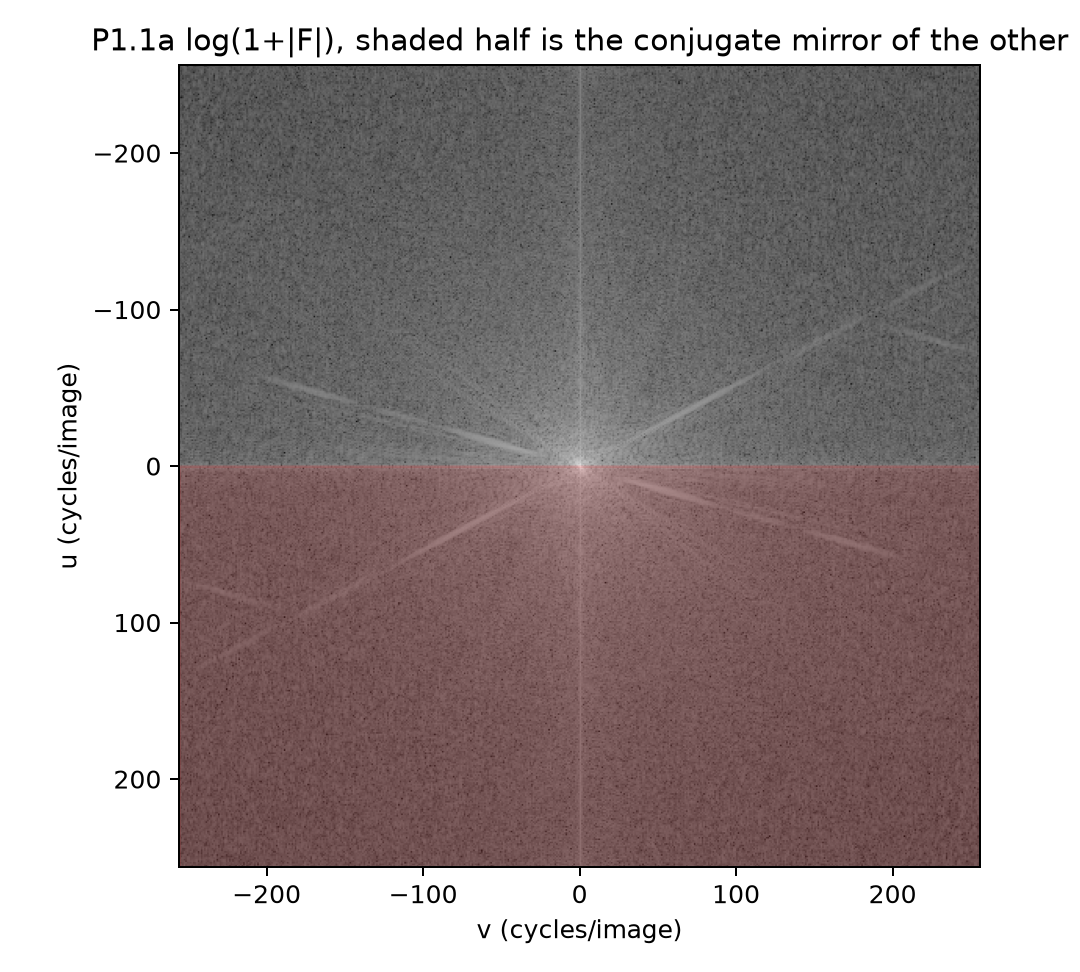
\includegraphics[width=0.45\linewidth]{problem_1/conjugate_symmetry.png}
\caption{Centred $\log(1+|F|)$ of \code{q1.png}. The shaded half is the
conjugate mirror of the other half.}
\label{fig:conj}
\end{figure}

\paragraph{(b) Shift and convolution theorems.} Substituting $x'=x-x_0$ in
\eqref{eq:dft} for a circular shift gives
$f(x-x_0,y-y_0)\leftrightarrow F(u,v)e^{-j2\pi(ux_0/M+vy_0/N)}$: the magnitude is
unchanged and the phase gains a linear ramp. Table~\ref{tab:shift} compares the
custom DFT of shifted copies of the test image (\code{np.roll}) with the
prediction, and lists the measured phase change at a few frequencies.

\begin{table}[H]
\centering
\begin{tabular}{lrrr}
\toprule
$(x_0,y_0)$ & $\max|F_s-F\cdot\text{ramp}|$ & relative & $\max\big||F_s|-|F|\big|$\\
\midrule
$(5,0)$ & $8.330\times10^{-9}$ & $2.46\times10^{-16}$ & $8.382\times10^{-9}$\\
$(0,17)$ & $1.542\times10^{-8}$ & $4.56\times10^{-16}$ & $5.588\times10^{-9}$\\
$(31,-12)$ & $1.201\times10^{-7}$ & $3.55\times10^{-15}$ & $7.451\times10^{-9}$\\
$(200,300)$ & $1.557\times10^{-6}$ & $4.60\times10^{-14}$ & $6.054\times10^{-9}$\\
\midrule
\multicolumn{4}{l}{phase change $\angle(F_s/F)$ in rad, shift $(31,-12)$ and $(200,300)$}\\
\midrule
$(u,v)$ & predicted & measured & $|$difference$|$\\
\midrule
$(1,0)$, shift $(31,-12)$ & $-0.380427$ & $-0.380427$ & $4.44\times10^{-16}$\\
$(50,-20)$, shift $(31,-12)$ & $-3.117049$ & $-3.117049$ & $3.55\times10^{-15}$\\
$(-100,140)$, shift $(31,-12)$ & $2.110758$ & $2.110758$ & $7.55\times10^{-15}$\\
$(0,1)$, shift $(200,300)$ & $2.601631$ & $2.601631$ & $8.88\times10^{-16}$\\
$(50,-20)$, shift $(200,300)$ & $1.178097$ & $1.178097$ & $5.33\times10^{-15}$\\
$(-100,140)$, shift $(200,300)$ & $0.196350$ & $0.196350$ & $1.87\times10^{-14}$\\
\bottomrule
\end{tabular}
\caption{2-D shift theorem on \code{q1.png} with the custom DFT. The full list of
20 phase checks is in \code{results/problem\_1/shift\_theorem\_table.txt}.}
\label{tab:shift}
\end{table}

The error grows with the shift because the ramp phase $2\pi(ux_0/M+vy_0/N)$ reaches
larger values before it is wrapped, so its round-off grows with it, but even at
$(200,300)$ the relative error is $4.6\times10^{-14}$.

For circular convolution
$g(x,y)=\sum_{m,n}h(m,n)f(x-m,y-n)$ with indices mod $M,N$, substituting into
\eqref{eq:dft} and swapping the sums gives $G=F\cdot H$, where $H$ is the DFT of the
kernel placed on the image grid with its origin at index $(0,0)$. The spatial side
was computed directly, one \code{np.roll} per kernel tap, and the frequency side as
$\text{idft2}(\text{dft2}(f)\,\text{dft2}(h))$ with the custom transforms.

\begin{table}[H]
\centering
\begin{tabular}{lrrrrr}
\toprule
Kernel & $\max|g_s-g_f|$ & $\max|g_s|$ & relative & $\max|\operatorname{Im} g_f|$ & $\max|G_s-FH|$\\
\midrule
box $3\times3$ & $2.501\times10^{-12}$ & $2.550\times10^{2}$ & $9.81\times10^{-15}$ & $3.145\times10^{-13}$ & $1.398\times10^{-8}$\\
Laplacian $5\times5$ & $6.412\times10^{-11}$ & $1.851\times10^{3}$ & $3.46\times10^{-14}$ & $5.699\times10^{-12}$ & $3.317\times10^{-8}$\\
random $7\times7$ & $4.093\times10^{-11}$ & $4.463\times10^{3}$ & $9.17\times10^{-15}$ & $4.736\times10^{-12}$ & $3.255\times10^{-7}$\\
\midrule
$(u,v)$, random kernel & \multicolumn{2}{r}{predicted $F H$} & \multicolumn{3}{r}{measured DFT of $f\circledast h$}\\
\midrule
$(0,0)$ & \multicolumn{2}{r}{$-5.627403\times10^{8}$} & \multicolumn{3}{r}{$-5.627403\times10^{8}$}\\
$(5,3)$ & \multicolumn{2}{r}{$6.338837\times10^{6}-8.990184\times10^{6}j$} & \multicolumn{3}{r}{$6.338837\times10^{6}-8.990184\times10^{6}j$}\\
$(100,-40)$ & \multicolumn{2}{r}{$-6.964199\times10^{3}-4.627895\times10^{3}j$} & \multicolumn{3}{r}{$-6.964199\times10^{3}-4.627895\times10^{3}j$}\\
$(-200,17)$ & \multicolumn{2}{r}{$-5.036941\times10^{3}+9.049523\times10^{3}j$} & \multicolumn{3}{r}{$-5.036941\times10^{3}+9.049523\times10^{3}j$}\\
\bottomrule
\end{tabular}
\caption{2-D circular convolution theorem on \code{q1.png}; $g_s$ is the direct
spatial result, $g_f$ the frequency-domain one and $G_s$ the DFT of $g_s$. The random kernel is
asymmetric (seed 7), so a flipped kernel or a misplaced origin would show up as a
large error.}
\label{tab:conv}
\end{table}

\paragraph{(c) Sinusoid parameter recovery.} The synthetic $256\times256$ image is
$f(x,y)=128+\sum_i A_i\cos(2\pi(u_ix+v_iy)/N+\phi_i)$ with the ground truth of
Table~\ref{tab:sin}. Writing each cosine as two complex exponentials shows that it
contributes $\tfrac{A_i}{2}MN\,e^{\pm j\phi_i}$ at $\pm(u_i,v_i)$ and nothing
elsewhere when $u_i,v_i$ are integers. The recovery therefore reads every peak
above $10^{-3}$ of the largest non-DC peak, keeps the member of each conjugate pair
with $u>0$ (or $u=0,v>0$), and returns $A=2|F|/MN$ and $\phi=\angle F$; the offset
is $F(0,0)/MN$. Only the spectrum is used, not the ground truth.

\begin{table}[H]
\centering
\begin{tabular}{lrrrrrr}
\toprule
$(u_i,v_i)$ cycles/image & $A$ true & $A$ found & $|\Delta A|$ & $\phi$ true & $\phi$ found & $|\Delta\phi|$\\
\midrule
$(6,10)$ & 50.00 & 50.0000000000 & $1.4\times10^{-14}$ & 0.785398 & 0.785398 & $3.6\times10^{-15}$\\
$(20,-14)$ & 30.00 & 30.0000000000 & $3.6\times10^{-15}$ & $-1.047198$ & $-1.047198$ & $1.3\times10^{-15}$\\
$(0,45)$ & 20.00 & 20.0000000000 & 0 & 2.000000 & 2.000000 & $4.4\times10^{-15}$\\
$(90,5)$ & 10.00 & 10.0000000000 & $3.6\times10^{-15}$ & $-2.500000$ & $-2.500000$ & $1.1\times10^{-14}$\\
\bottomrule
\end{tabular}
\caption{Ground truth and recovered parameters. Exactly four peaks were found and
the recovered offset is 128.0000000000.}
\label{tab:sin}
\end{table}

\textbf{Resolution limit.} An $N$-point DFT samples the spectrum of the finite
signal at $u/N$ cycles per pixel, so the grid spacing is
$\Delta f=1/N$ cycles/pixel, i.e.\ one cycle per image ($1/256=0.003906$ here).
The origin is the finite observation window: the $N$ samples are the infinite
signal times a length-$N$ rectangle, so every spectral line is convolved with the
Dirichlet kernel $D_N(\nu)=\sin(\pi N\nu)/(N\sin(\pi\nu))$, whose main lobe is
$2/N$ wide. Two components closer than about $1/N$ merge into one lobe, and no
amount of zero padding separates them, because zero padding only samples the same
blurred spectrum more finely. Fig.~\ref{fig:sin} shows both effects. Two cosines
$0.5$ cycles/image apart give one main peak even in a $16\times$ zero-padded
spectrum, while $1.5$ cycles/image apart they give two. A single cosine at the
off-grid frequency $10.5$ is read as amplitude $31.07$ and $32.56$ from the two
nearest bins against a true 50; the Dirichlet prediction for a half-bin offset is
$50\,|D_N(1/2N)|=31.83$. Its energy also leaks, so 33 bins exceed one grey level.

\begin{figure}[H]
\centering
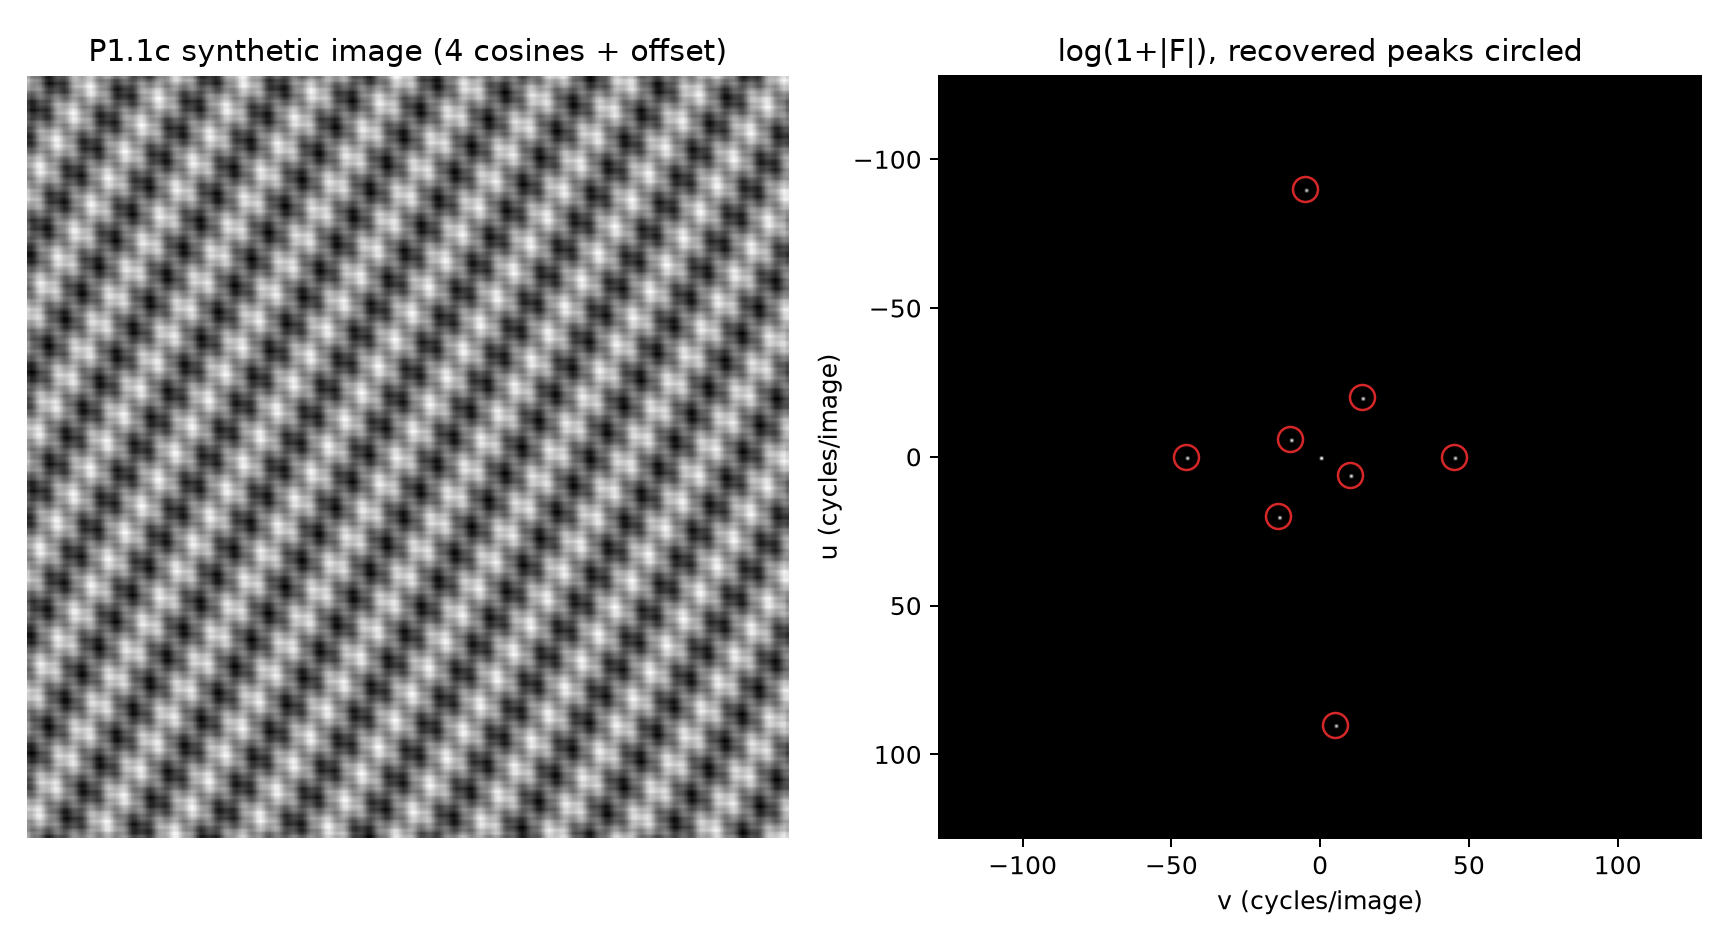
\includegraphics[width=0.72\linewidth]{problem_1/sinusoid_recovery.png}\\
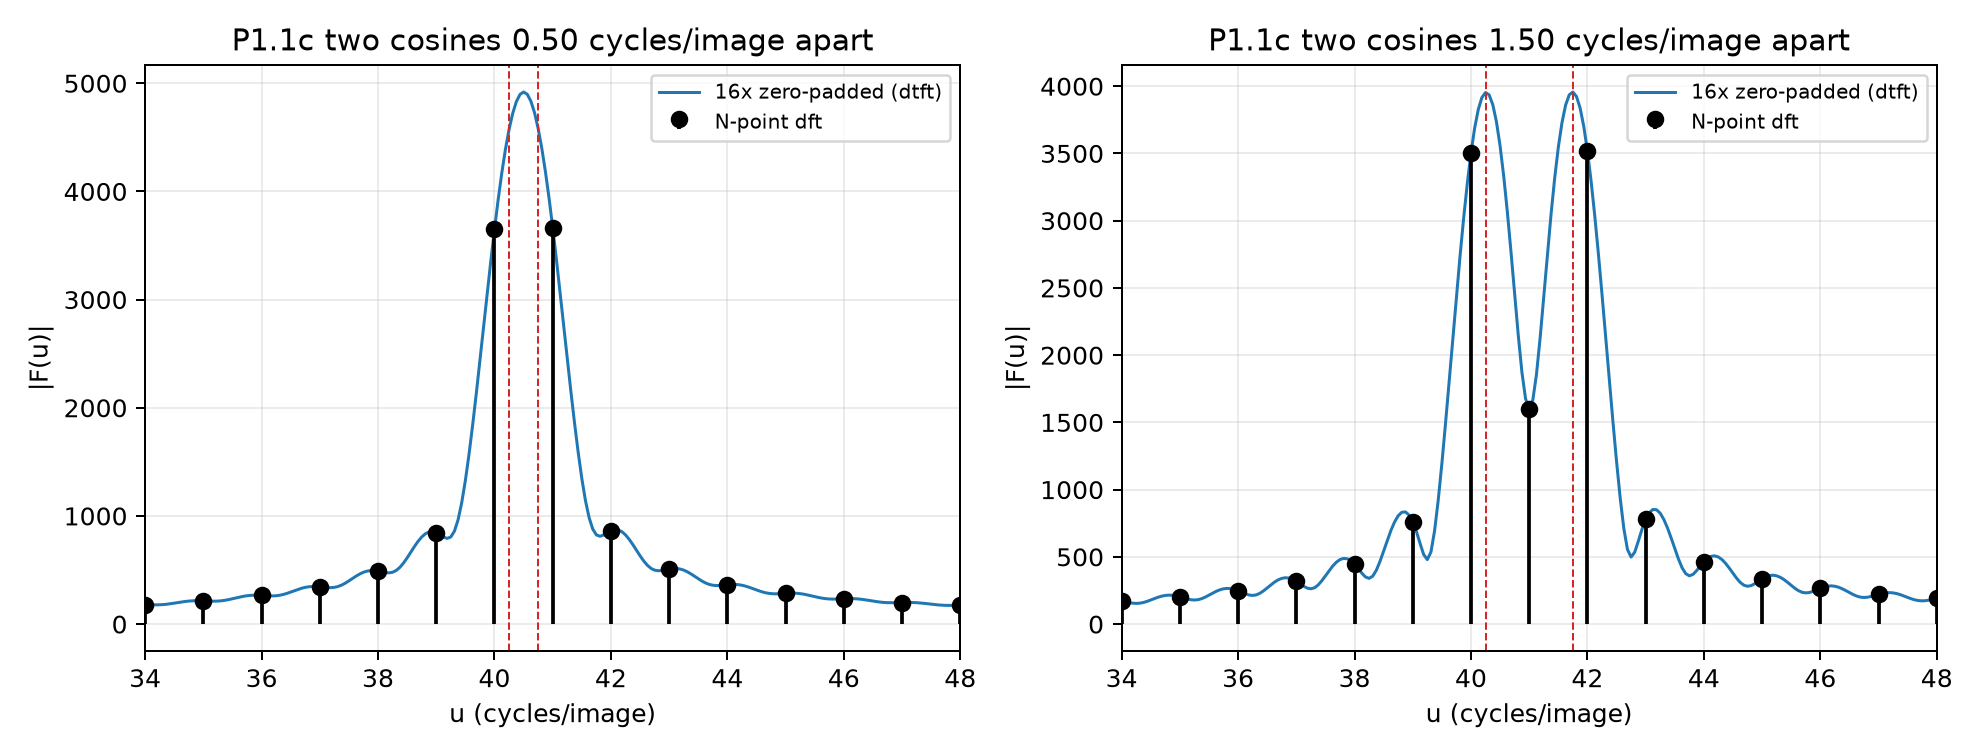
\includegraphics[width=0.85\linewidth]{problem_1/resolution_limit.png}
\caption{Top: synthetic image and its centred log spectrum with the recovered peaks
circled. Bottom: two cosines $0.5$ and $1.5$ cycles/image apart, 256-point DFT
(stems) and $16\times$ zero-padded spectrum (line).}
\label{fig:sin}
\end{figure}

\subsection{Phase versus magnitude}

That phase carries most of the structure of an image is a classical observation
\cite{oppenheim}; this section predicts and measures how much.


\textbf{Prediction.} The analytical prediction is in
\code{docs/predictions/p1\_2\_phase\_magnitude\_prediction.md}, written on
2026-10-23 at 16:28 and committed at 16:29 (commit \code{3c9e956}), seven minutes
before the experiment code was committed (\code{164d182}, 16:36). In short: for
uniform white noise $n$ of the same size, $|N(u,v)|$ is close to Rayleigh
distributed away from DC, so $|N|=\mu(1+\epsilon)$ with
$\operatorname{var}\epsilon=4/\pi-1=0.273$. By superposition
$r=\text{idft}(|N|e^{j\phi})=\mu p+\mu\,\text{idft}(\epsilon e^{j\phi})+\text{const}$,
where $p=\text{idft}(e^{j\phi})$ is the flat-magnitude image. By the shift theorem a
feature at $(x_k,y_k)$ carries the linear phase $e^{-j2\pi(ux_k/M+vy_k/N)}$, and a
linear phase with flat magnitude inverts to an impulse at $(x_k,y_k)$, so $p$ should
concentrate at the positions of edges and lines (equivalently $p=f\circledast
\text{idft}(1/|F|)$, a whitening high-pass). The second term is $p$ convolved with
the white field $\text{idft}(\epsilon)$, a stationary speckle, and Parseval predicts
its energy relative to the first as $\operatorname{E}\epsilon^2=0.273$, so a
least-squares fit $r=cp+\text{residual}$ should leave a residual of 27\,\% of
$\|cp\|^2$ and $\operatorname{corr}(r,p)\approx1/\sqrt{1.273}=0.89$.

\begin{figure}[H]
\centering
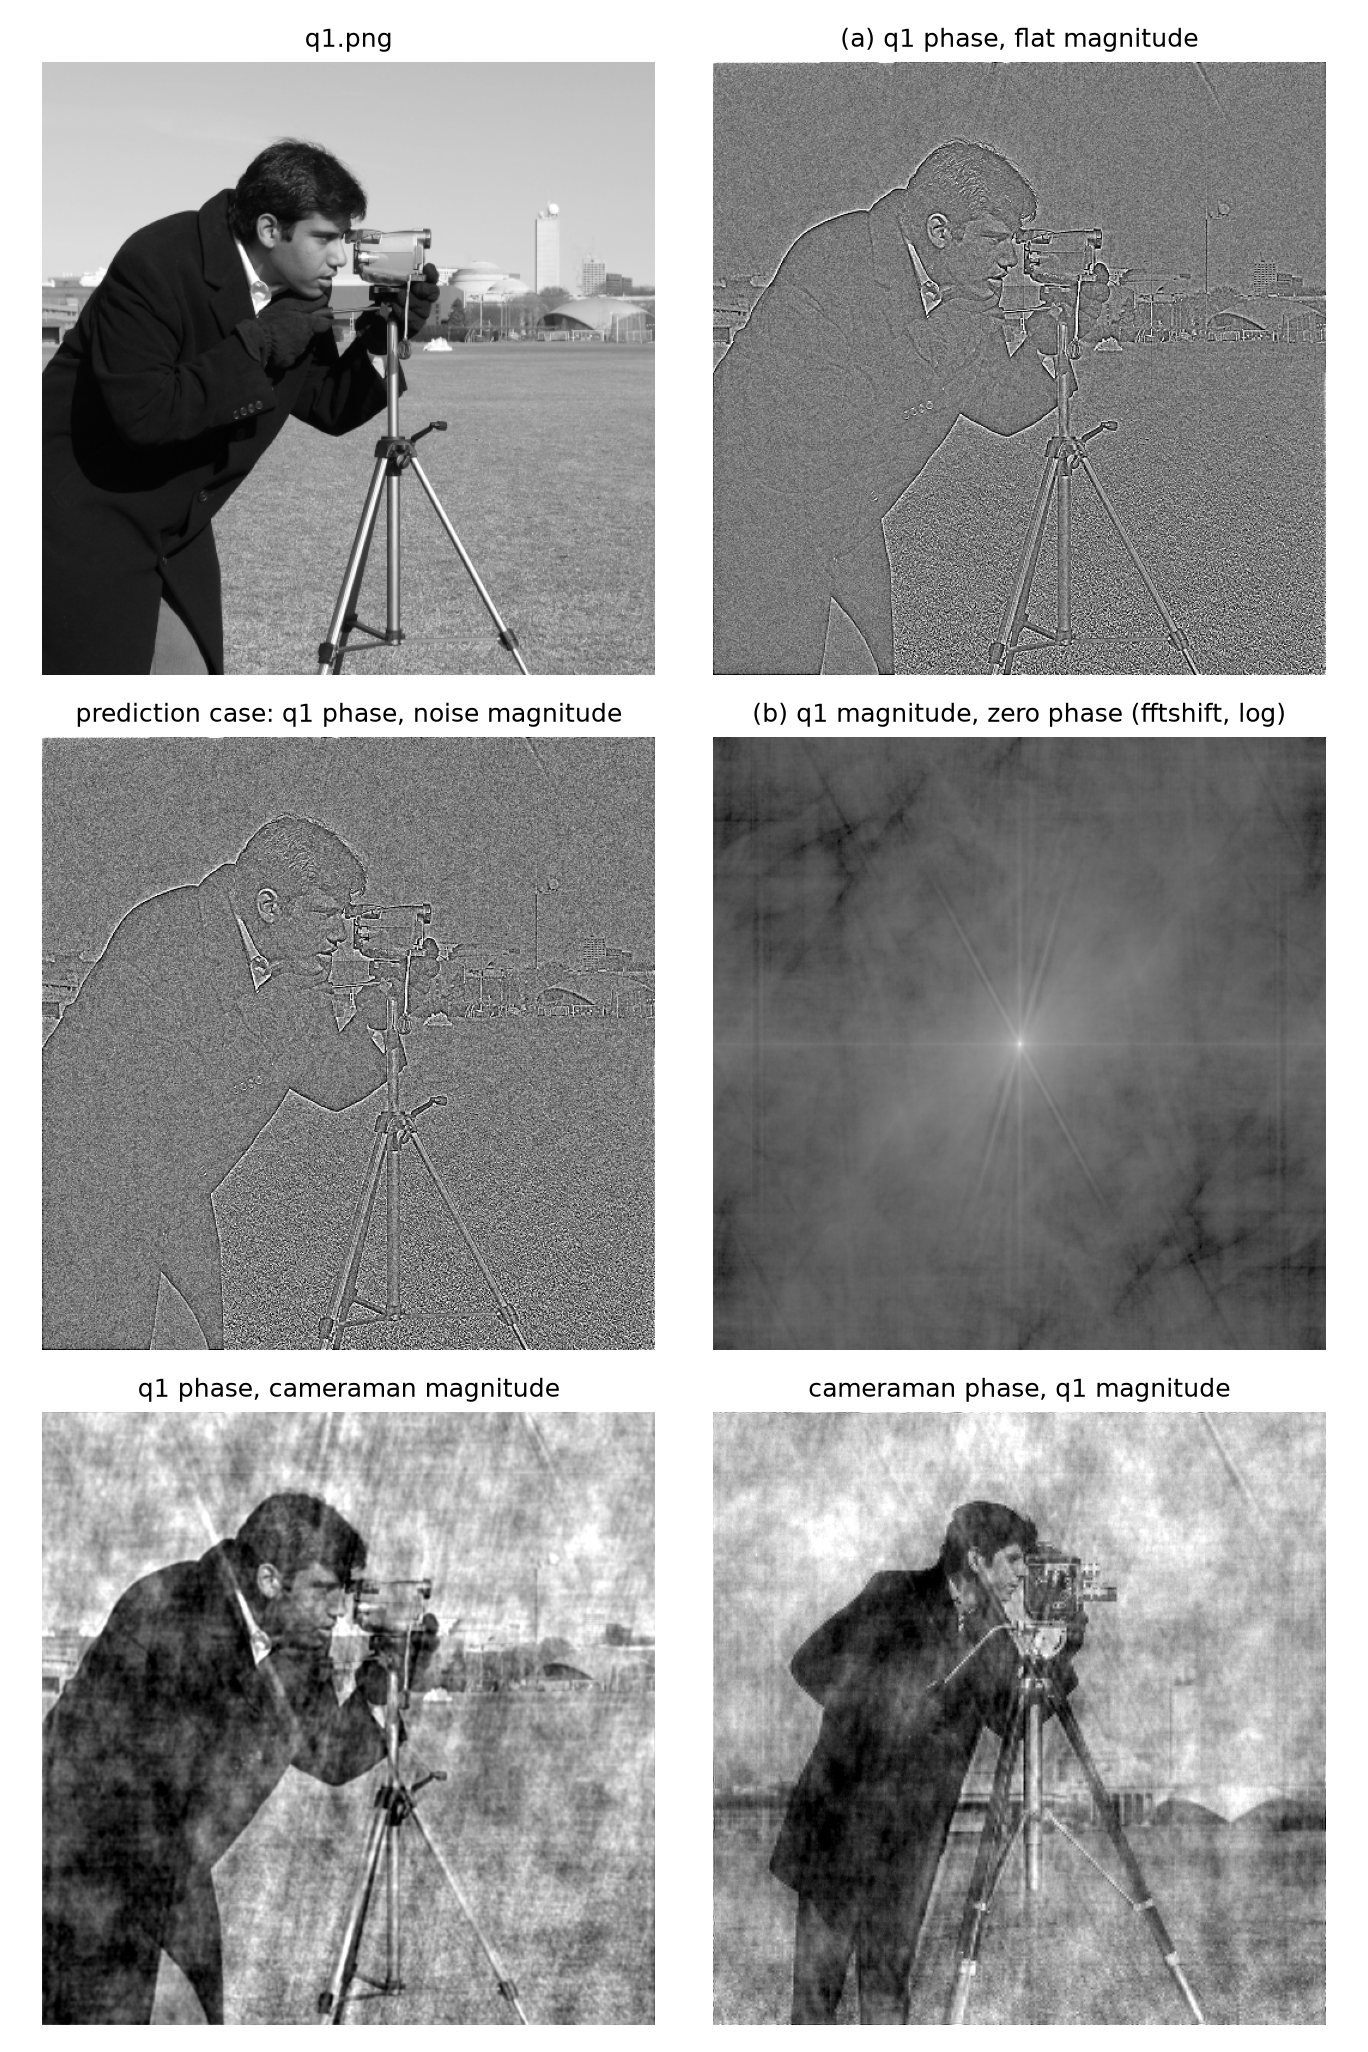
\includegraphics[width=\linewidth]{problem_1/phase_magnitude.png}
\caption{Phase and magnitude experiments on \code{q1.png} (custom transforms).
Each panel is stretched between its 0.5 and 99.5 percentiles; the zero-phase
panel is $\log(1+|r_0|)$ after \code{fftshift}.}
\label{fig:phase}
\end{figure}

\paragraph{(a) Flat magnitude.} The phase-only image (Fig.~\ref{fig:phase}, top
middle) shows the outline of the photographer, the coat edge, the tripod legs and
the buildings at their true positions as thin bright and dark lines, and has no
large-scale shading: $\operatorname{corr}(p,f)=0.18$ while
$\operatorname{corr}(|p|,|\nabla f|)=0.48$. The noise-magnitude case matches the
prediction closely (Table~\ref{tab:phase}). The measured $\operatorname{var}\epsilon$
is 0.2744, the residual-to-structure energy ratio is 0.2744 against the predicted
0.273, and $\operatorname{corr}(r,p)=0.8858$ against 0.89. The two ratios agree to
four digits because, with the same phase, the residual is exactly the
$\epsilon$-weighted part of the spectrum.

\begin{table}[H]
\centering
\begin{tabular}{lrr}
\toprule
Quantity & predicted & measured\\
\midrule
$\operatorname{var}\epsilon$ of the noise magnitude (DC excluded) & $4/\pi-1=0.2732$ & 0.2744\\
energy(residual) / energy($cp$) & 0.273 & 0.2744\\
$\operatorname{corr}(r,p)$ & 0.89 & 0.8858\\
$\operatorname{corr}(|p|,|\nabla f|)$ / $\operatorname{corr}(|r|,|\nabla f|)$ & speckle lowers it & 0.4806 / 0.4077\\
\bottomrule
\end{tabular}
\caption{Prediction against measurement for the noise-magnitude reconstruction
(uniform noise, seed 2026).}
\label{tab:phase}
\end{table}

One part of the prediction did not hold. It said flat areas such as the sky would
go to a uniform grey. They carry a fine grain instead (Fig.~\ref{fig:phase} and
\code{phase\_magnitude\_zoom.png}). The sky in the photograph is not exactly flat:
it has small sensor and compression fluctuations, and dividing by $|F|$ boosts the
high frequencies where those fluctuations live as much as it boosts edges.
Whitening cannot tell a weak high-frequency texture from a strong one.

Flat magnitude isolates phase more cleanly than swapping magnitudes between two
natural images because a natural magnitude is not neutral. Natural spectra all fall
off roughly like $1/\rho$, so combining the phase of \code{q1} with the magnitude of
\code{cameraman.tif} gives an image that correlates 0.906 with \code{q1}
(Fig.~\ref{fig:phase}, bottom left), which looks like strong evidence for phase.
But that output is shaped by two things at once: the phase, and a magnitude with
its own envelope and its own orientation streaks. A flat magnitude has no envelope
and no orientation, so whatever survives in the output can only have come from the
phase.

\paragraph{(b) Zero phase.} Setting $\angle F=0$ gives
$r_0=\text{idft}(|F|)$. Since $|F|$ is real and even, $r_0$ is real and
point-symmetric: the measured $\max|\operatorname{Im}r_0|/\max|\operatorname{Re}r_0|$
is $1.6\times10^{-16}$ and $\max|r_0(x,y)-r_0(-x,-y)|=9.1\times10^{-13}$. All
cosines are in phase at the origin, so the maximum sits at $(0,0)$ with value
$\sum|F|/MN=7071.55$, and the mean of $r_0$ equals the mean of $f$ (129.06),
because the DC term is untouched. None of the photograph's structure survives,
because positions live in the phase. The prediction expected a sharp peak plus a
faint axis cross from the border discontinuities of the periodic extension. The
cross is there: the lines $x=0$ and $y=0$ hold 3.35\,\% of the energy outside
radius 8, although they are only 0.39\,\% of the pixels. The peak is less compact
than predicted, with only 21\,\% of the mean-removed energy within radius 8. The
figure shows why: there are additional streaks through the origin parallel to the
tripod legs. A long straight edge puts a ridge of energy through the centre of
$|F|$, perpendicular to the edge, and the inverse transform of a ridge through the
origin is a line through the origin perpendicular to it, i.e.\ parallel to the
original edge. The prediction considered only the image border and missed that
interior straight edges behave the same way.

\subsection{Padding, wraparound and computational overhead}

\paragraph{(a) Wraparound and minimal padding.} The $5\times5$ Laplacian
$\begin{psmallmatrix}0&0&1&0&0\\0&1&2&1&0\\1&2&-16&2&1\\0&1&2&1&0\\0&0&1&0&0\end{psmallmatrix}$
was applied to \code{q1.png} as an unpadded circular convolution (kernel origin at
the image origin) and as a zero-padded linear convolution cropped to the image size
(\code{mode="same"}). The linear version matches \code{scipy.signal.convolve2d} to
$4.5\times10^{-12}$. The two differ by up to 1608 grey levels, in exactly 4080
pixels: the band of $(M-1)/2=2$ pixels along every border
($512^2-508^2=4080$). Inside that band they agree to $5\times10^{-12}$
(Table~\ref{tab:wrap}). In the band, the circular result mixes in pixels from the
opposite side of the image. Fig.~\ref{fig:wrap} shows this at the top-left corner,
and with a $31\times31$ box blur, whose 15-pixel band (29820 pixels) is wide
enough to see: the bottom of the photograph bleeds into the top rows.

Linear convolution of an $N$-sample signal with an $M$-sample kernel has support
$N+M-1$. A $P$-point circular convolution of the zero-padded signals equals the
linear result aliased with period $P$, $g_P[x]=\sum_k g_\text{lin}[x+kP]$, and the
copies do not overlap if and only if $P\ge N+M-1$. For an $N\times N$ image and an
$M\times M$ kernel the minimal padded size is therefore
\begin{equation}
N_{x,\text{pad}}=N_{y,\text{pad}}=N+M-1\quad(=516\text{ here}).
\end{equation}
If only the \code{same}-size crop is needed, the aliased samples can be allowed to
land in the $(M-1)/2$ rows that the crop discards, so $P\ge N+(M-1)/2$ suffices. The
measurements agree: $P=512$ and 513 corrupt 4080 and 2044 pixels of the crop, and
every $P\ge514$ is exact to round-off.

\begin{table}[H]
\centering
\begin{tabular}{rrr}
\toprule
$P$ & $\max|g_P-g_\text{linear}|$ & corrupted pixels\\
\midrule
512 & $1.608\times10^{3}$ & 4080\\
513 & $3.490\times10^{2}$ & 2044\\
514 & $6.821\times10^{-12}$ & 0\\
515 & $8.911\times10^{-12}$ & 0\\
516 & 0 & 0\\
520 & $5.144\times10^{-12}$ & 0\\
1024 & $5.230\times10^{-12}$ & 0\\
\bottomrule
\end{tabular}
\caption{\code{same}-cropped result on a $P\times P$ zero-padded grid against the
exact linear convolution, $5\times5$ Laplacian on \code{q1.png}.}
\label{tab:wrap}
\end{table}

\begin{figure}[H]
\centering
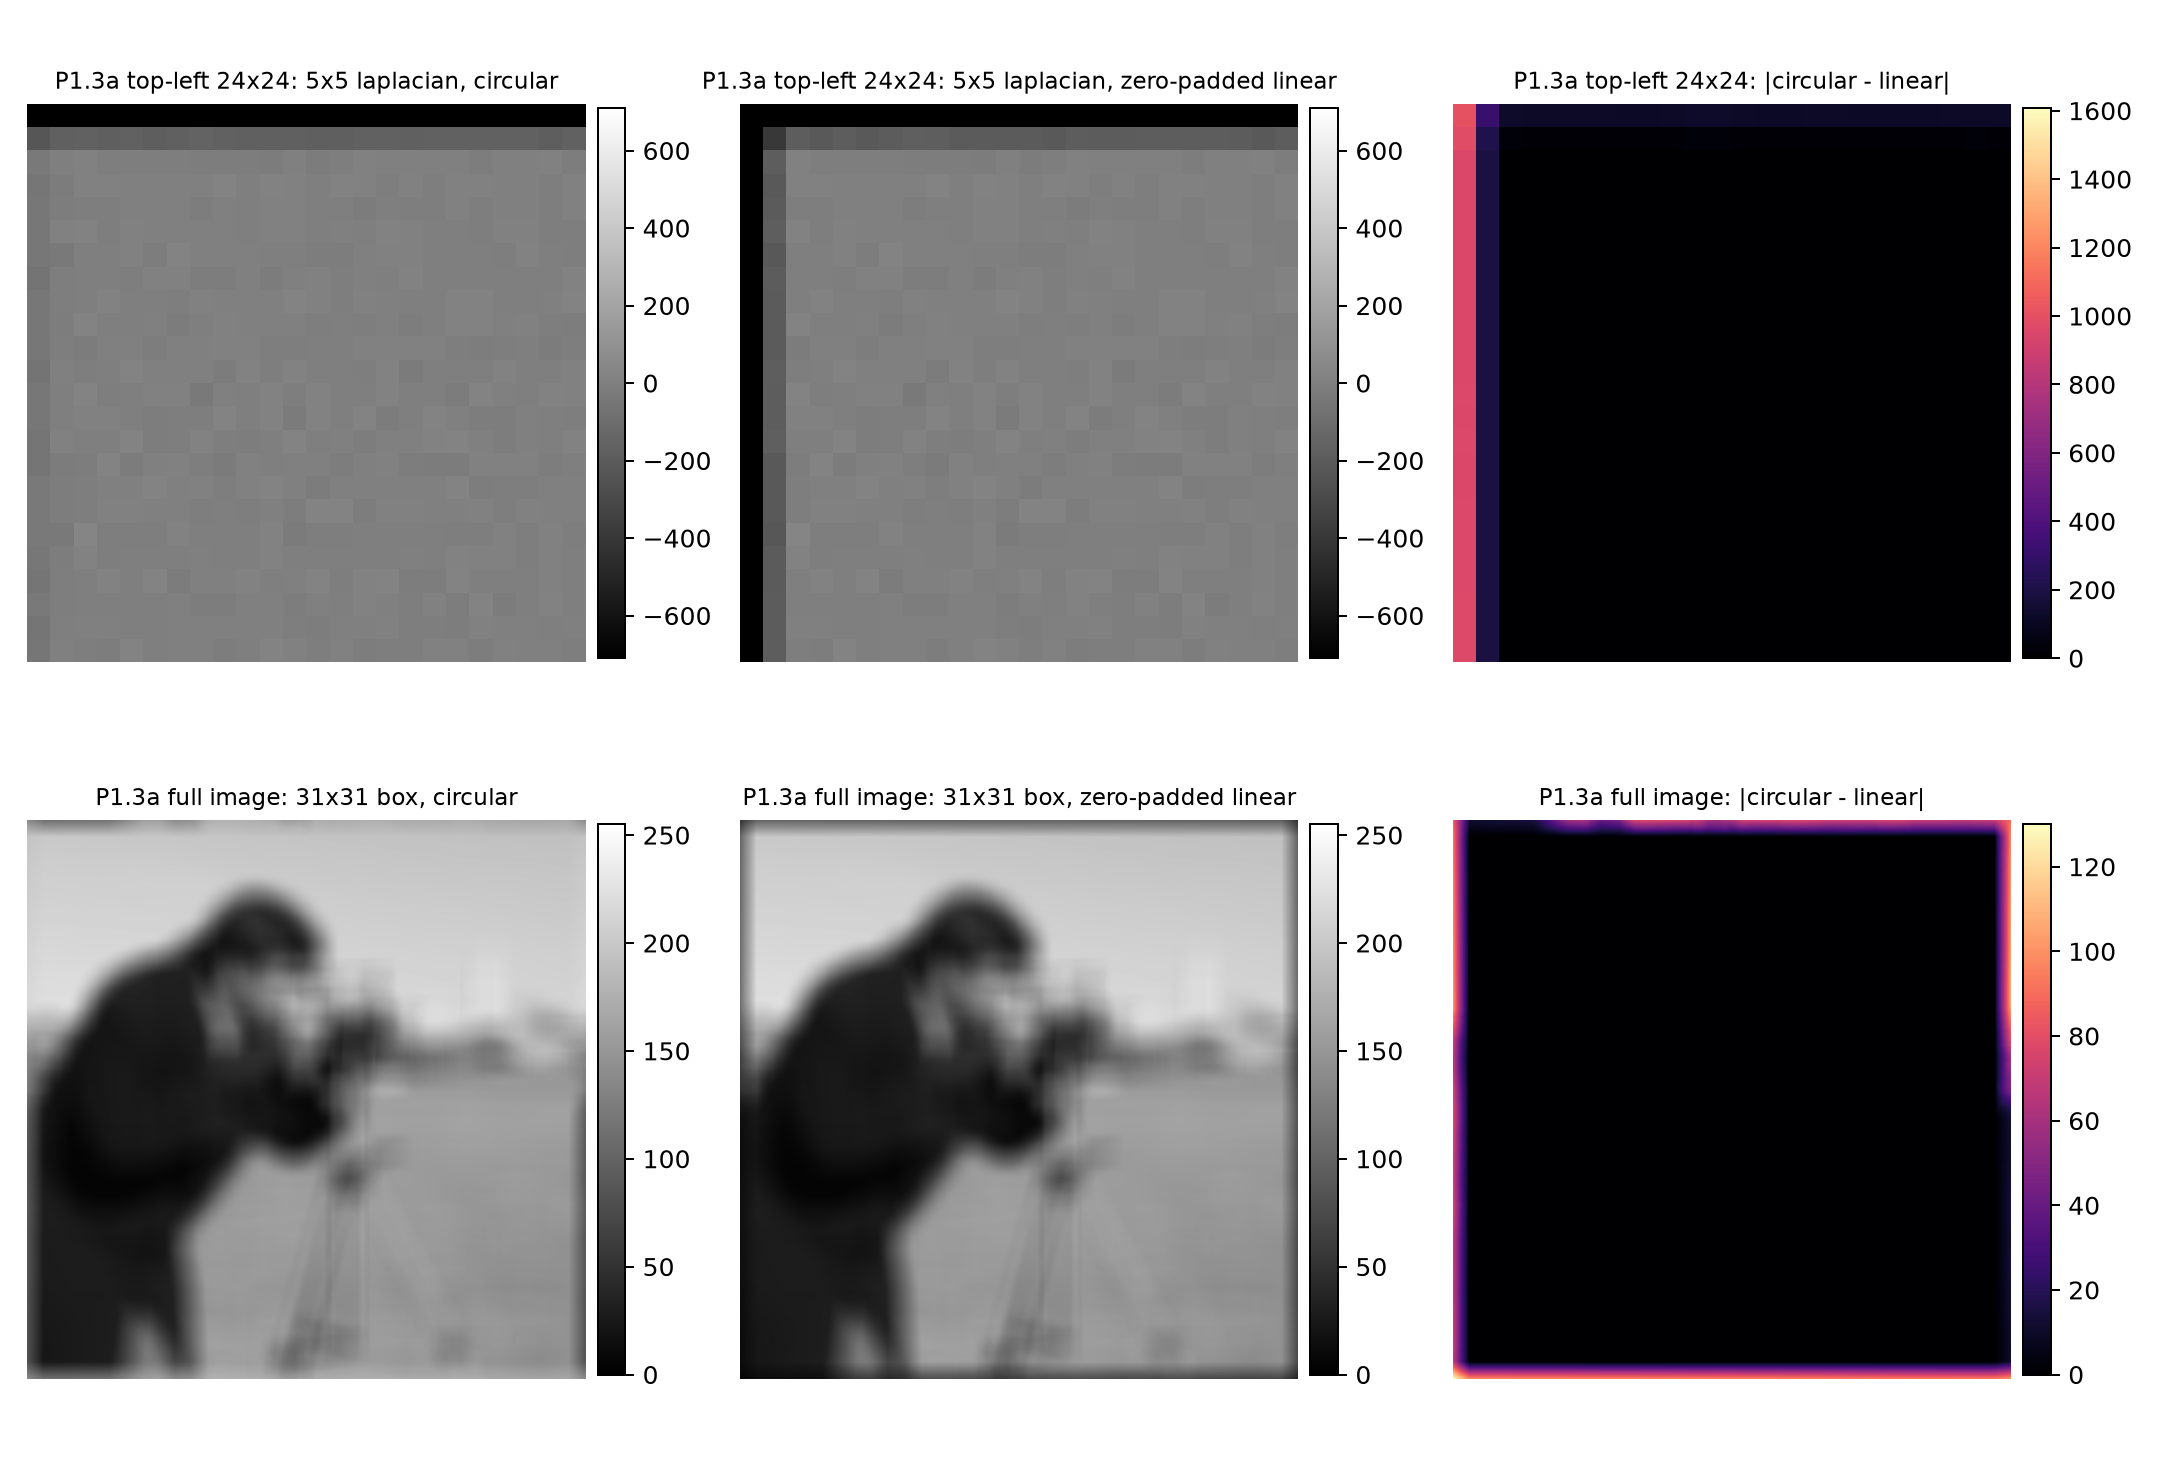
\includegraphics[width=0.9\linewidth]{problem_1/wraparound.png}
\caption{Top: $24\times24$ top-left corner for the $5\times5$ Laplacian. Bottom:
the same comparison with a $31\times31$ box blur over the whole image.}
\label{fig:wrap}
\end{figure}

\paragraph{(b) Cost of padding.} Padding both arrays from $N^2$ to $P^2$ multiplies
every array in the pipeline by $(P/N)^2$: 1.0157 for the minimal $P=516$ and 4 for
the $P=2N$ rule used in Problem 2. The tracemalloc peaks in Table~\ref{tab:pad}
follow this exactly (16.00 MiB to 16.25 MiB to 64.00 MiB). The FFT cost
$O(P^2\log P)$ grows by $(P/N)^2\log P/\log N$: 1.017 for 516 and 4.44 for 1024.
The measured times follow the model only roughly, because FFT speed depends on the
prime factors of $P$. $516=2^2\cdot3\cdot43$ contains the prime 43 and takes
1.40$\times$ the time of $N=512$, while 525 and 540 have only small factors and run
faster than 512 itself. Why the power of two is slower here was not investigated;
strided column passes hitting the same cache sets is one possible reason.
\code{scipy.signal.fftconvolve} handles this trade-off internally. It pads each axis
to the full linear size and then up to \code{next\_fast\_len}$(516,\text{real}=\text{True})=540$,
a 5-smooth size, spending 11\,\% more memory than the minimum to avoid the slow
prime factor, and uses real-input FFTs (\code{rfftn}) that only compute half the
spectrum, which is the redundancy from 1.1a. It took 3.07 ms against 9.40 ms for
the minimal-size complex pipeline.

\begin{table}[H]
\centering
\begin{tabular}{lrlrrrrrr}
\toprule
Grid & $P$ & factors & $(P/N)^2$ & ops ratio & time (ms) & time ratio & MiB & mem.\ ratio\\
\midrule
$N$ (circular) & 512 & $2^9$ & 1.0000 & 1.0000 & 6.723 & 1.000 & 16.00 & 1.000\\
$N+M-1$ & 516 & $2^2\cdot3\cdot43$ & 1.0157 & 1.0170 & 9.400 & 1.398 & 16.25 & 1.016\\
next fast, real & 540 & $2^2\cdot3^3\cdot5$ & 1.1124 & 1.1219 & 6.084 & 0.905 & 17.80 & 1.112\\
next fast, complex & 525 & $3\cdot5^2\cdot7$ & 1.0514 & 1.0557 & 5.581 & 0.830 & 16.83 & 1.051\\
$2N$ (Problem 2) & 1024 & $2^{10}$ & 4.0000 & 4.4444 & 31.140 & 4.632 & 64.00 & 4.000\\
\bottomrule
\end{tabular}
\caption{Cost of the padded pipeline (\code{fft2} of image and kernel, product,
\code{ifft2}), $N=512$, $M=5$. ``ops ratio'' is $P^2\log P/(N^2\log N)$; MiB is the
tracemalloc peak. Times are medians of 41 interleaved runs.}
\label{tab:pad}
\end{table}

\paragraph{Conclusion.} The matrix DFT agrees with \code{numpy.fft} to float64
round-off, and the symmetry, shift and convolution properties hold to the same
precision. Phase carries where things are and magnitude carries how much of each
frequency there is, and the Rayleigh-based prediction for the noise-magnitude
reconstruction was confirmed to within 0.5\,\%. Exact linear convolution needs a
grid of $N+M-1$; in practice the size is rounded up to a fast FFT length.

\section{Frequency-domain filtering: ideal, Butterworth, Gaussian}

Everything in this problem goes through the zero-padded pipeline from 1.3
\cite{gonzalez}. I pad the image with zeros at the bottom and right to
$P\times P$ with $P=2N$, centre the spectrum with \code{fftshift}, multiply by a
real zero-phase $H(u,v)$, invert, keep the real part and crop. For the two
non-square images (\code{text\_gaps} is $444\times508$, \code{thumb\_print} is
$962\times1026$) I use a square grid with $P=2\max(\text{rows},\text{cols})$,
so that a given $D(u,v)$ means the same frequency along both axes. A distance
$D$ in frequency bins is $D/P$ cycles per pixel. The step image $s(x,y)$ is a
$256\times256$ square of value $B=200$ on a background $A=50$, covering rows and
columns 128 to 383.

\subsection{Filter construction and transfer functions}

\code{make\_filter(kind, P, D0, n=None, highpass=False)} in
\code{src/problem\_2/filters.py} has the interface the handout asks for. It
builds $D(u,v)=\sqrt{(u-P/2)^2+(v-P/2)^2}$ and then one of
\begin{equation}
H_\text{ILPF}=\begin{cases}1&D\le D_0\\0&D>D_0\end{cases},\qquad
H_\text{BLPF}=\frac{1}{1+(D/D_0)^{2n}},\qquad
H_\text{GLPF}=e^{-D^2/2D_0^2},\qquad H_\text{HP}=1-H_\text{LP}.
\end{equation}
Fig.~\ref{fig:tf} plots all six on one axis.

\begin{figure}[H]
\centering
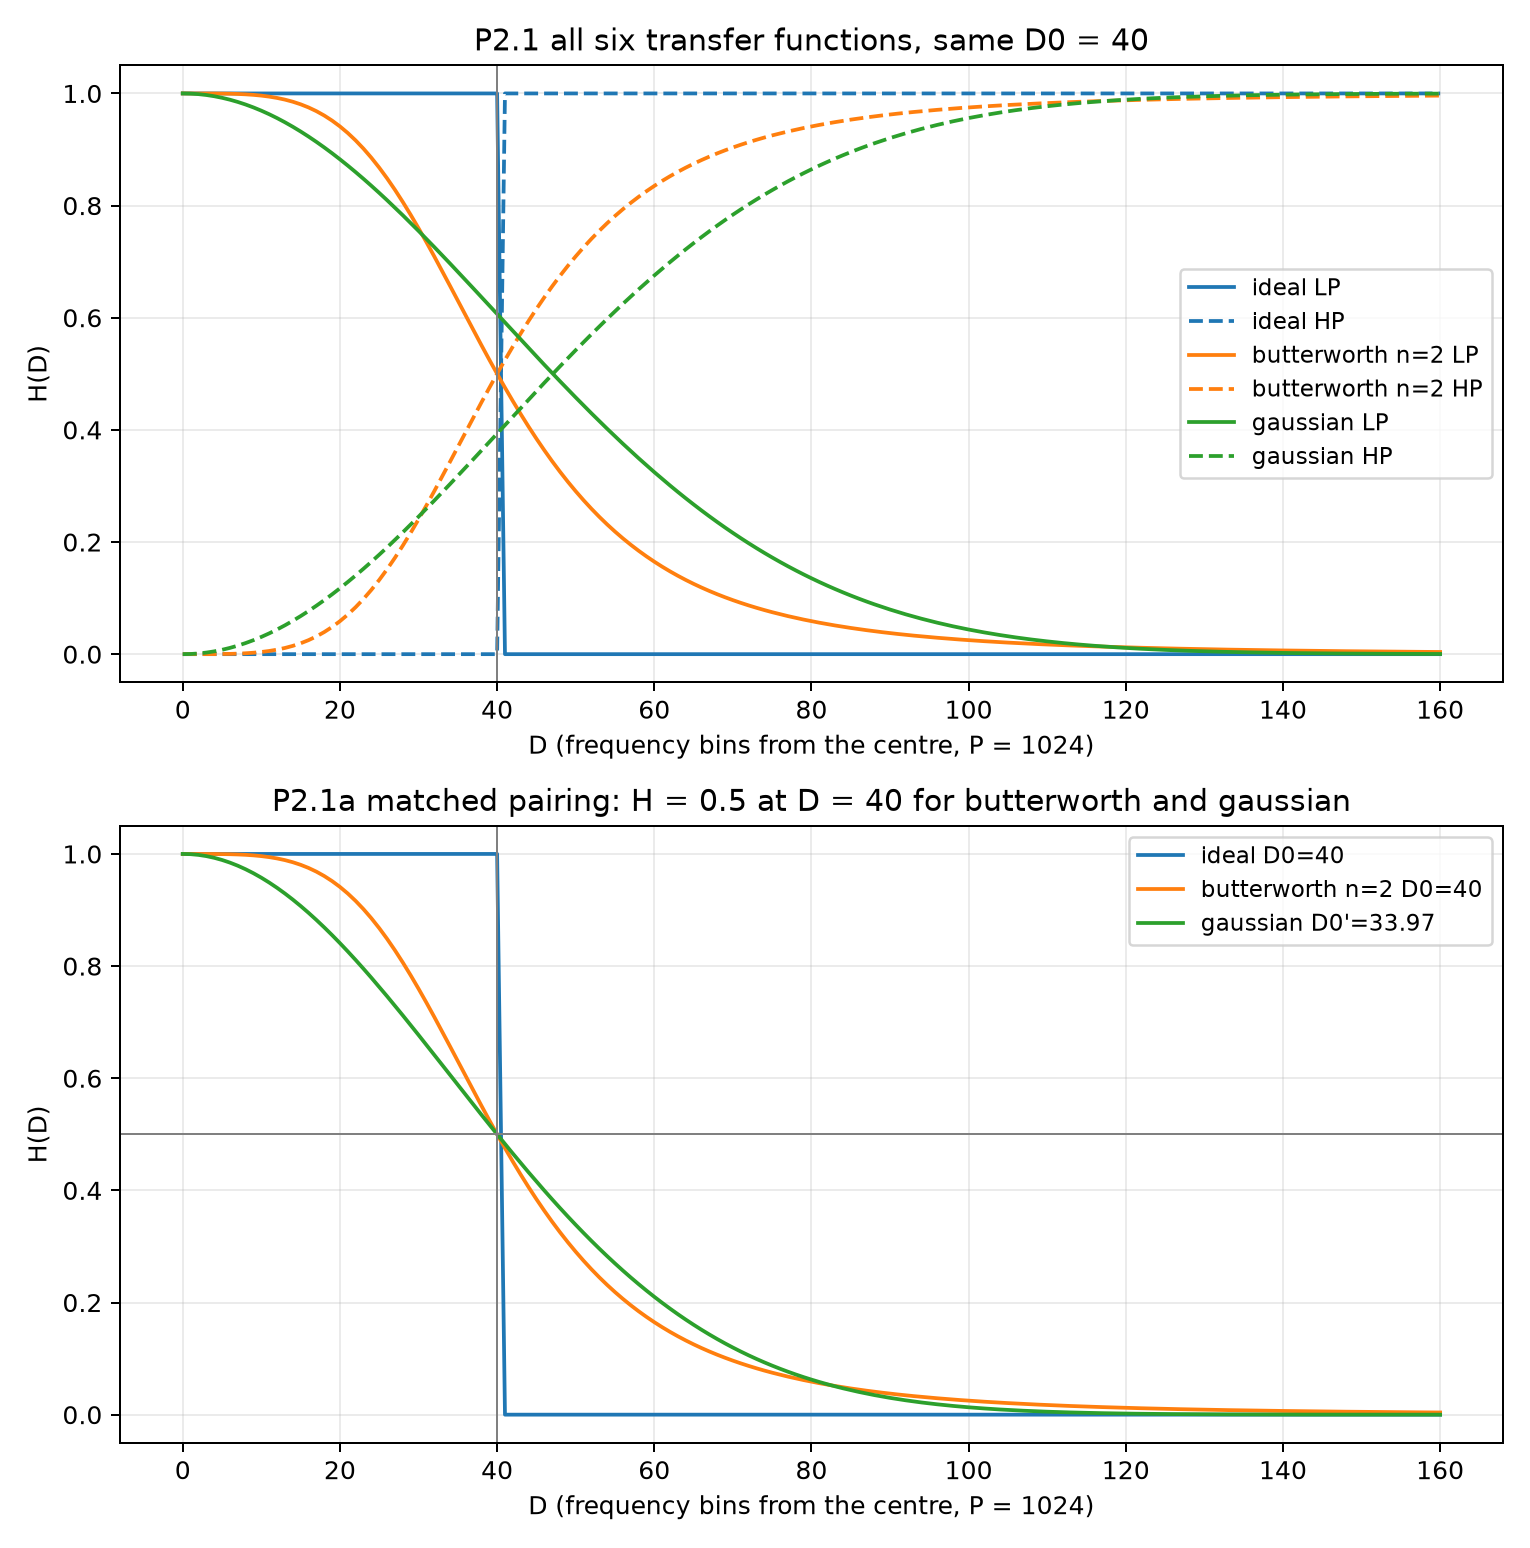
\includegraphics[width=0.95\linewidth]{problem_2/transfer_functions.png}
\caption{Left: the six transfer functions against $D$ (frequency bins from the
centre) for the same $D_0=40$ with $P=1024$ and Butterworth $n=2$. Right: the
matched pairing used in every later comparison.}
\label{fig:tf}
\end{figure}

\paragraph{(a) Cutoff semantics.} Putting $D=D_0$ into each formula gives
$H_\text{ILPF}=1$ (the definition includes $D=D_0$), $H_\text{BLPF}=1/(1+1)=1/2$
for every order, and $H_\text{GLPF}=e^{-1/2}=0.606531$. \code{make\_filter}
returns exactly these values (\code{cutoff\_semantics.txt}). So the same number
$D_0$ means three different things: the last frequency the ideal filter passes,
the half-amplitude point of the Butterworth filter, and the one standard
deviation point of the Gaussian. Comparing them at equal $D_0$ is therefore not
fair. To put the Gaussian's half-amplitude point at the Butterworth cutoff
$D_0$, I solve
\begin{equation}
e^{-D_0^2/2D_0'^2}=\tfrac12\;\Longrightarrow\;\frac{D_0^2}{2D_0'^2}=\ln2\;\Longrightarrow\;
D_0'=\frac{D_0}{\sqrt{2\ln2}}=\frac{D_0}{1.177410}.
\end{equation}
For $D_0=40$ this gives $D_0'=33.9729$, and the built filter has $H=0.500000$
at $D=40$. \textbf{From here on, every Gaussian is described by its
half-amplitude radius $D_0$ and built with $D_0'$.}

\paragraph{(b) Energy-based cutoff.} For the characters pattern padded to
$P=1376$ I computed $\alpha(r)$ by sorting all bins by $D$ and accumulating
$|F|^2$.

\begin{table}[H]
\centering
\begin{tabular}{rrr}
\toprule
target $\alpha$ & radius $r$ (bins) & $\alpha(r)$\\
\midrule
90\,\% & 15.30 & 90.0033\,\%\\
95\,\% & 45.54 & 95.0002\,\%\\
99\,\% & 409.04 & 99.0000\,\%\\
99.5\,\% & 558.74 & 99.5000\,\%\\
\bottomrule
\end{tabular}
\caption{Radii that enclose a given share of the spectral power, characters
pattern, $P=1376$ (\code{power\_retention.txt}, curve in
\code{power\_retention.png}).}
\label{tab:power}
\end{table}

The DC bin alone holds 22.4\,\% of the power and radius 5 already holds
81.6\,\%. The pattern is mostly a flat light background with mean 207, and the
zero padding turns the whole image into one big bright rectangle, so most of the
power just describes the mean level and the outline of that rectangle. Edges put
a small amount of power into a very large number of high frequencies: the last
5\,\% of the power lies beyond $r=45.5$ and the last 1\,\% beyond $r=409$. Those
frequencies are what we actually see, though. They carry the position and
sharpness of every stroke and bar, and the eye cares much more about edges than
about the little power they hold. Fig.~\ref{fig:grid} shows that keeping 95\,\%
of the power still leaves the text badly blurred.

\paragraph{(c) Inverse design.} From $H(10)=16/17$,
\[
1+\Big(\frac{10}{D_0}\Big)^{2n}=\frac{17}{16}\;\Longrightarrow\;\Big(\frac{10}{D_0}\Big)^{2n}=\frac1{16},
\]
and from $H(40)=1/17$, $(40/D_0)^{2n}=16$. Dividing the second by the first
removes $D_0$:
\[
\Big(\frac{40}{10}\Big)^{2n}=4^{2n}=\frac{16}{1/16}=256=4^4\;\Longrightarrow\;n=2.
\]
Then $(10/D_0)^4=1/16$ gives $10/D_0=1/2$, so $D_0=20$. For at most 1\,\% at
$D=2D_0$ I need
\[
\frac{1}{1+2^{2n}}\le0.01\;\Longrightarrow\;4^n\ge99\;\Longrightarrow\;n\ge\frac{\ln99}{\ln4}=3.3147,
\]
so the smallest integer order is $n=4$. As a check,
\code{make\_filter("butterworth", 256, 20, n=2)} gives $H(10)=0.941176=16/17$
and $H(40)=0.058824=1/17$, and $H(2D_0)$ is
$0.200000, 0.058824, 0.015385, 0.003891$ for $n=1,2,3,4$: order 3 misses the
1\,\% target and order 4 meets it (\code{inverse\_design.txt}).

\subsection{Ringing: prediction, measurement and reconciliation}

\textbf{The prediction.} I wrote it on 23 October 2026 at 16:29 IST and
committed it at 16:29 (\code{3c9e956}). Its first line first said 16:31 by
mistake, and I corrected that line eight seconds later in \code{4acb1a0}. No code
had been committed at that point: the first code commit, with the shared FFT
helpers, is at 16:36 (\code{f6ef560}), and the Problem 2 filters and experiments
followed at 16:45 (\code{3618251}, \code{d801bfd}). The full text is
in Appendix~\ref{app:pred-ringing} and in
\code{docs/predictions/p2\_2\_ringing\_prediction.pdf}. The derivation goes as
follows.

Near the middle row and away from the corners, the image looks like a function
of $x$ only, $s(x,y)\approx g(x)$. The DFT of such an image is non-zero only on
the line $v=0$, because the sum over $y$ of $e^{-j2\pi vy/P}$ vanishes for every
$v\ne0$. The filter therefore acts only through its slice $H(u,0)$, and the
filtered row is the 1-D convolution of $g$ with $h(x)=\mathcal F^{-1}\{H(u,0)\}$.
For the ideal filter the slice is a box of half-width $f_c=D_0/P$ cycles/pixel,
so in the continuous model $h(x)=\sin(2\pi f_cx)/(\pi x)$. A step of height
$B-A$ at $x_e$ is $A+(B-A)\,\mathbf 1[x>x_e]$, and convolving it with $h$ gives
$A$ plus $(B-A)$ times the area of $h$ to the left of $x-x_e$:
\begin{equation}
g(x)=A+(B-A)\int_{-\infty}^{x-x_e}\frac{\sin(2\pi f_ct)}{\pi t}\,dt
=A+(B-A)\Big[\tfrac12+\tfrac1\pi\Si\big(2\pi f_c(x-x_e)\big)\Big],\qquad
\Si(z)=\int_0^z\frac{\sin t}{t}\,dt .
\label{eq:si}
\end{equation}
The second form uses the substitution $t'=2\pi f_ct$ and the fact that each half
of $\int_{-\infty}^{\infty}\sin t/t\,dt=\pi$ contributes $\pi/2$. $\Si$ has its
largest value at $z=\pi$, $\Si(\pi)=1.851937$, so

\begin{itemize}
\item the overshoot is $100(\Si(\pi)/\pi-\tfrac12)=8.949\,\%$ of $B-A$ for every
$D_0$ (the Gibbs value), and
\item the first peak sits where $2\pi f_cd=\pi$, i.e.\ $d=1/(2f_c)=P/(2D_0)$
pixels from the edge.
\end{itemize}

The prediction also listed where the measurement could differ: the discrete
passband ($2D_0+1$ frequencies, a Dirichlet kernel whose first zero is at
$P/(2D_0+1)$), sampling of the peak on integer columns, ripples from the other
edge and from the jump to zero at the image border (about $P/(2\pi^2D_0r)$ of
each jump at distance $r$, largest for $D_0=10$), the finite height of the
square, and the corners. For the Gaussian the slice inverts to a positive
Gaussian with $\sigma_s=P/(2\pi D_0)$ (derived in 2.2(d)), the edge becomes
$A+(B-A)\Phi((x-x_e)/\sigma_s)$ with $\Phi$ the normal CDF, and the predicted
overshoot is 0 because $\Phi$ is monotone.

\paragraph{(a) Ideal filter.} Table~\ref{tab:ringing} gives the measurements on
row 255. The left edge is at $x_e=127.5$, so sampled distances are
half-integers; the ``parabolic'' column refines the peak position with a
parabola through the three samples around it.

\begin{table}[H]
\centering
\begin{tabular}{rrrrrrrr}
\toprule
$D_0$ & OS (\%) & predicted & $d$ sampled & $d$ parabolic & $P/2D_0$ & $P/(2D_0+1)$ & $\max g$\\
\midrule
10 & 3.440 & 8.95 & 50.5 & 50.45 & 51.20 & 48.76 & 205.160\\
20 & 11.447 & 8.95 & 26.5 & 26.20 & 25.60 & 24.98 & 217.170\\
40 & 8.269 & 8.95 & 12.5 & 12.76 & 12.80 & 12.64 & 212.403\\
80 & 8.779 & 8.95 & 6.5 & 6.43 & 6.40 & 6.36 & 213.169\\
\bottomrule
\end{tabular}
\caption{Ideal low-pass on the step image, $P=1024$, profile row 255. Distances
in pixels. The right edge gives the same sampled distances.}
\label{tab:ringing}
\end{table}

The peak positions match $P/(2D_0)$ to within 0.75 pixel at every cutoff. The
overshoot is close to 8.95\,\% for $D_0=40$ and 80 but clearly off at $D_0=10$
(3.4\,\%) and 20 (11.4\,\%). To find out which of the predicted effects causes
this, I filtered the same row two more ways (Table~\ref{tab:recon}). ``1-D row''
filters the row as if the image did not change along $y$, so it keeps the second
edge and the padding jumps but nothing two-dimensional. ``Isolated'' is a single
edge on a grid 16 times longer with the same $f_c=D_0/P$, so no other edge is
close.

\begin{table}[H]
\centering
\begin{tabular}{rrrrrr}
\toprule
$D_0$ & OS 2-D (\%) & OS 1-D row (\%) & $d$ 1-D row & OS isolated (\%) & $d$ isolated\\
\midrule
10 & 3.440 & 7.775 & 44.18 & 8.949 & 51.20\\
20 & 11.447 & 9.210 & 25.61 & 8.955 & 25.61\\
40 & 8.269 & 9.721 & 12.81 & 8.948 & 12.81\\
80 & 8.779 & 9.425 & 6.44 & 9.036 & 6.44\\
\bottomrule
\end{tabular}
\caption{Reconciling the overshoot: the full 2-D image, the same row filtered in
1-D, and an isolated edge.}
\label{tab:recon}
\end{table}

The isolated edge gives the continuous result almost exactly: 8.949\,\% and
$d=51.20=P/(2D_0)$ at $D_0=10$. So \eqref{eq:si} is right for a lone edge, and
the discrete frequency grid on its own changes very little once the grid is
this fine. Two other effects pull the measurement away. The 1-D row adds the
other edge 256 pixels away and the $-50$ padding jumps 128 pixels away. Their
ripples move the overshoot by $-1.2$ to $+0.8$ percentage points and, at
$D_0=10$, move the peak to 44.2 pixels, which is the size the prediction
estimated from the $1/(2\pi^2D_0r)$ ripple amplitude. The rest of the gap
between the 1-D row and the 2-D image comes from the finite height of the
square. Its spectrum is not confined to $v=0$ but fills a band about
$P/256=4$ bins wide, and on the slice at height $v$ the ideal cutoff is only
$\sqrt{D_0^2-v^2}$, which matters a lot when $D_0=10$. The top and bottom edges
also send their own ripples down to row 255. Both effects shrink as $D_0$ grows,
which is why the measurements approach 8.95\,\% at $D_0=80$. The discrete
passband refinement $P/(2D_0+1)$ is too small to see next to these interference
effects at $P=1024$.

\textbf{Near a corner} the 1-D argument does not hold at all, because the image
changes in both directions and the ripples from the vertical and the horizontal
edge add up. The maximum inside the top-left quadrant of the square lies on the
diagonal, at the 1-D peak distance from both edges (Table~\ref{tab:corner}), and
the overshoot there is 18.0 to 19.2\,\% for $D_0\ge20$. That is close to
$(1+0.0895)^2-1=18.7\,\%$, which is what two independent Gibbs peaks would give
for a separable filter. The circular ideal filter is not separable, which is one
reason the match is not exact.

\begin{table}[H]
\centering
\begin{tabular}{rrrrr}
\toprule
$D_0$ & $\max g$ & OS (\%) & position (row, col) & distance from both edges (px)\\
\midrule
10 & 222.686 & 15.124 & (181, 181) & 53.5\\
20 & 227.040 & 18.026 & (154, 154) & 26.5\\
40 & 228.824 & 19.216 & (141, 141) & 13.5\\
80 & 228.193 & 18.795 & (134, 134) & 6.5\\
\bottomrule
\end{tabular}
\caption{Maximum of the filtered image near the top-left corner of the square.}
\label{tab:corner}
\end{table}

\begin{figure}[H]
\centering
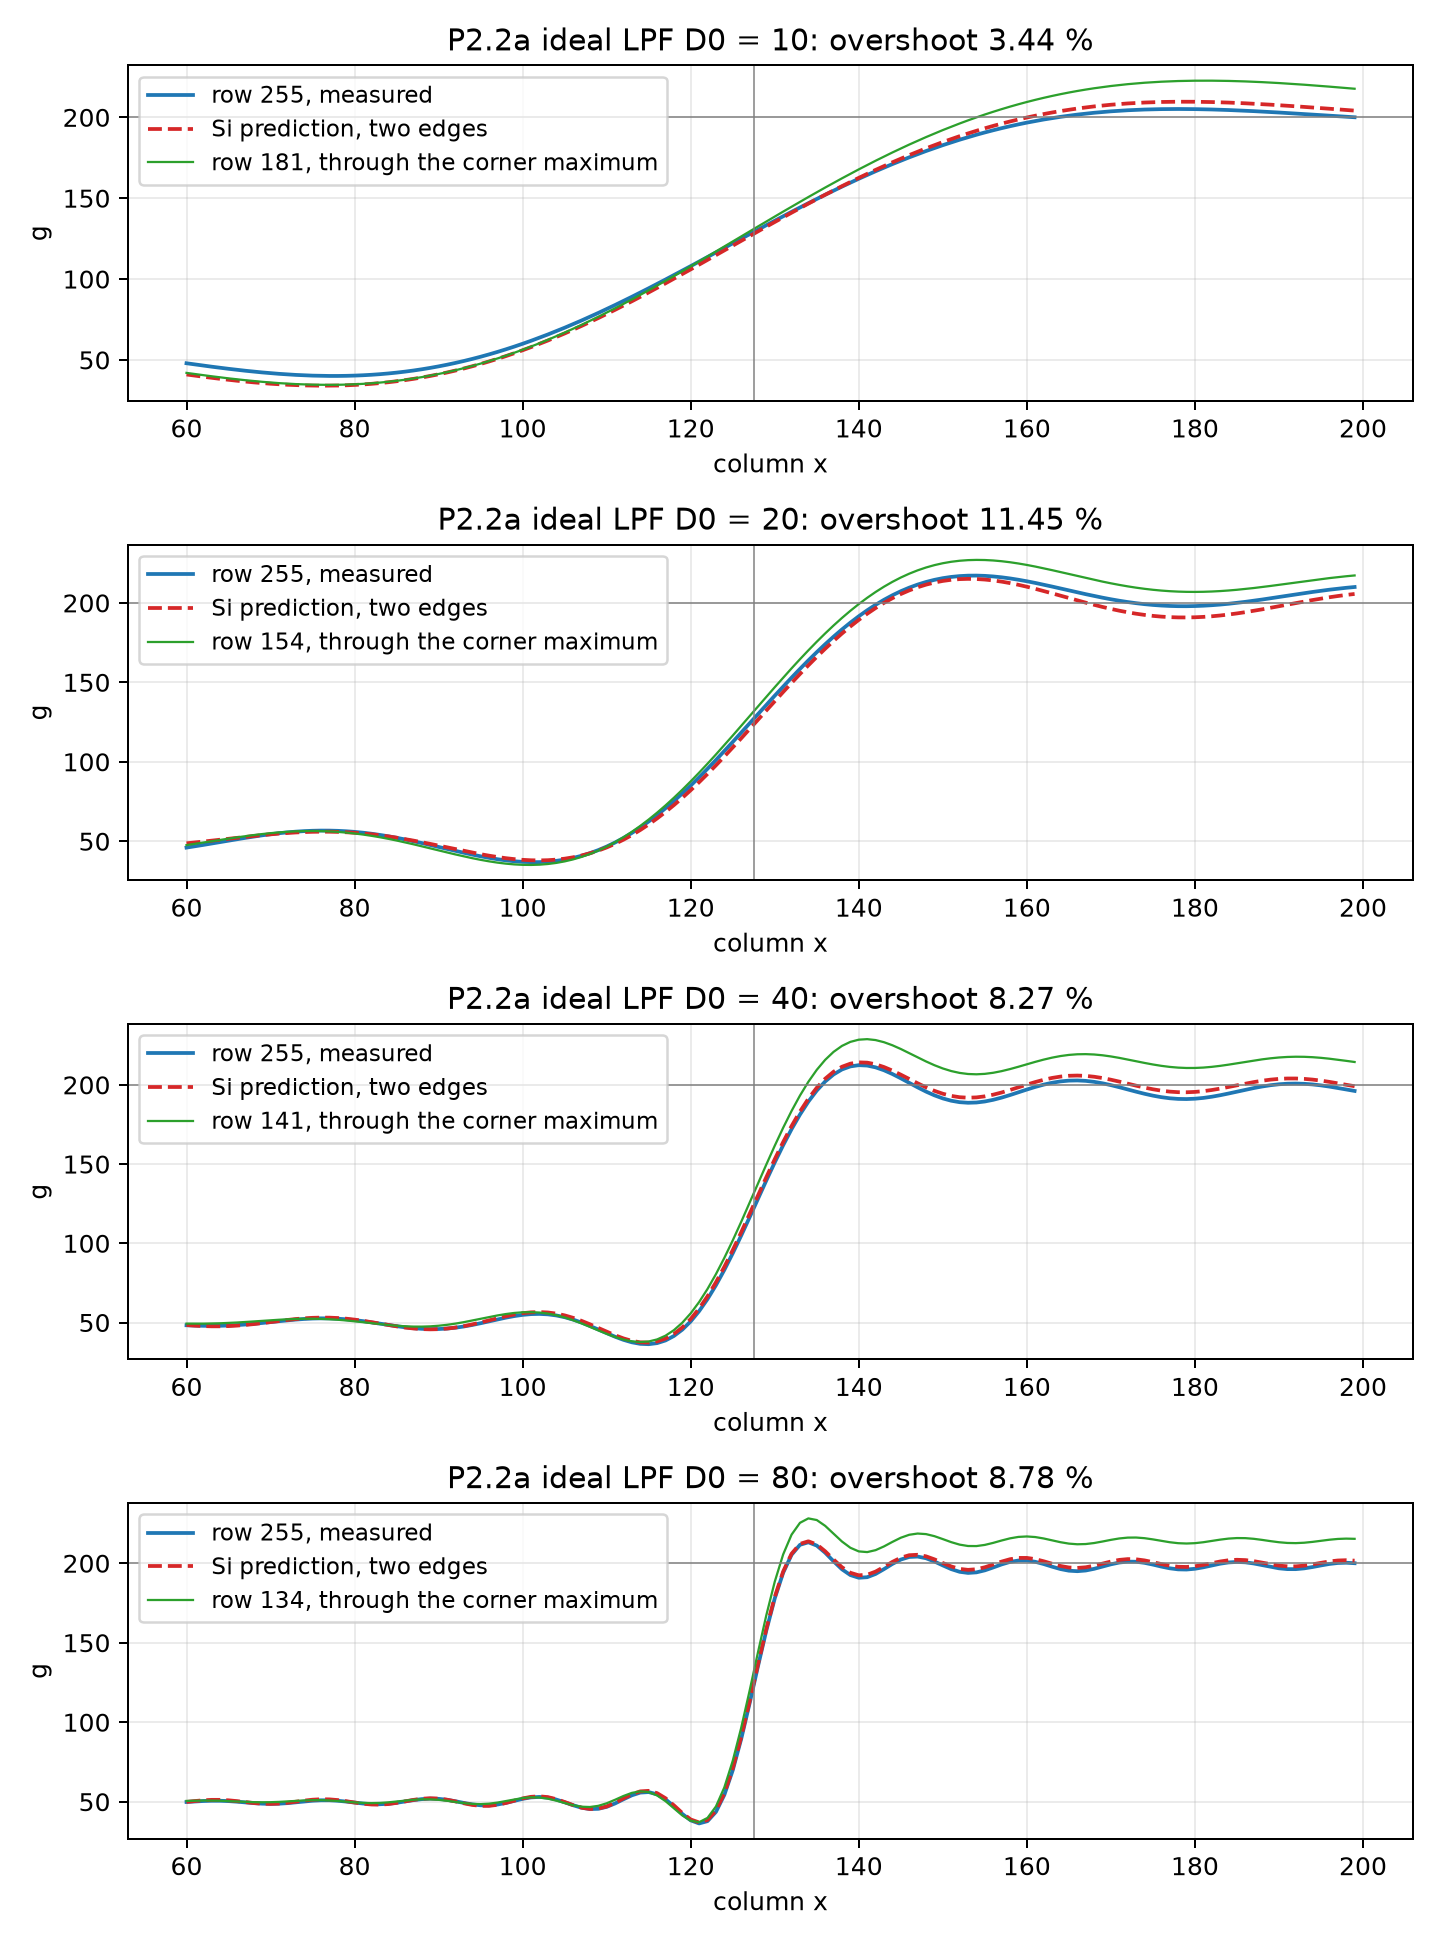
\includegraphics[width=0.95\linewidth]{problem_2/ideal_ringing_profiles.png}
\caption{Grey level against column: the measured row 255 (blue), the two-edge
prediction from \eqref{eq:si} (red, dashed) and the row through the corner
maximum (green), one panel per $D_0$.}
\label{fig:ringing}
\end{figure}

\paragraph{(b) Butterworth order sweep.} With $D_0=40$ the overshoot grows with
the order (Table~\ref{tab:bw}). The 1-D kernel $h(x)$ is the inverse DFT of the
central slice $H(u,0)$ of the $1024\times1024$ filter.

\begin{table}[H]
\centering
\begin{tabular}{lrrrrr}
\toprule
Filter & OS (\%) & $d$ (px) & $\min h$ & $\max h$ & $|\min h|/\max h$\\
\midrule
Butterworth $n=1$ & 0.0000 & none & $-2.938\times10^{-7}$ & $1.1663\times10^{-1}$ & $2.5191\times10^{-6}$\\
Butterworth $n=2$ & 3.3590 & 13.5 & $-3.749\times10^{-3}$ & $8.6763\times10^{-2}$ & $4.3207\times10^{-2}$\\
Butterworth $n=3$ & 5.6032 & 12.5 & $-7.906\times10^{-3}$ & $8.1812\times10^{-2}$ & $9.6639\times10^{-2}$\\
Butterworth $n=5$ & 7.4995 & 12.5 & $-1.253\times10^{-2}$ & $7.9425\times10^{-2}$ & $1.5775\times10^{-1}$\\
Butterworth $n=10$ & 8.4865 & 12.5 & $-1.569\times10^{-2}$ & $7.8447\times10^{-2}$ & $1.9995\times10^{-1}$\\
Butterworth $n=20$ & 8.4337 & 12.5 & $-1.661\times10^{-2}$ & $7.8205\times10^{-2}$ & $2.1236\times10^{-1}$\\
ideal & 8.2688 & 12.5 & $-1.719\times10^{-2}$ & $7.9102\times10^{-2}$ & $2.1730\times10^{-1}$\\
Gaussian $D_0=40$ & 0.0000 & none & $-1.388\times10^{-17}$ & $9.7915\times10^{-2}$ & $1.4\times10^{-16}$\\
Gaussian $D_0'=33.97$ & 0.0000 & none & $-6.939\times10^{-18}$ & $8.3161\times10^{-2}$ & $8.3\times10^{-17}$\\
\bottomrule
\end{tabular}
\caption{Overshoot and kernel ratio against Butterworth order, $D_0=40$,
$P=1024$. Every kernel sums to 1.00000.}
\label{tab:bw}
\end{table}

For $n=1$ the slice $1/(1+(u/D_0)^2)$ is a Lorentzian, and its inverse
transform is a two-sided exponential $\propto e^{-2\pi D_0|x|/P}$, which is
positive everywhere. The tiny minimum of $-2.9\times10^{-7}$ only comes from
cutting the slice off at $|u|=P/2$, and the overshoot is zero. For $n\ge2$ the
slice is flatter at the top and falls faster, and a transfer function that
falls faster than a Lorentzian needs negative lobes in its kernel. The ratio
$|\min h|/\max h$ rises from 0.043 at $n=2$ to 0.212 at $n=20$, close to the
ideal filter's 0.217, and the overshoot rises with it from 3.36\,\% towards the
ideal limit. The measured values for $n=10$ and 20 (8.49 and 8.43\,\%) sit a bit
above the measured ideal (8.27\,\%) because the same 2-D and other-edge effects
as in 2.2(a) act here too; the isolated-edge limit is 8.95\,\%.

\emph{Proof that a non-negative kernel cannot overshoot.} Let $h(k)\ge0$ with
$\sum_kh(k)=1$, and let the step $s$ only take values in $[A,B]$. The output
$g(x)=\sum_kh(k)\,s(x-k)$ is a weighted average of values of $s$ with
non-negative weights that add up to one, so
\[
A=\sum_kh(k)\,A\;\le\;g(x)\;\le\;\sum_kh(k)\,B=B\quad\text{for every }x.
\]
So $\max g\le B$ and the overshoot is at most zero. The same argument works in
2-D, so it covers the 2-D Butterworth filter with $n=1$ and the Gaussian, whose
kernels are positive. Ringing therefore needs negative lobes, and the kernel
ratio measures how big they are.

\paragraph{(c) Visual comparison.} Fig.~\ref{fig:grid} applies the three
families to the characters pattern at the four radii of Table~\ref{tab:power}.
At $r=15.3$ and 45.5 the ideal filter shows the ripples predicted above. The
insets in Fig.~\ref{fig:insets} mark two places: bright and dark bands parallel
to each side of the large black square, and light gaps between the vertical
bars that rise above the background level. Butterworth $n=2$ shows a faint
version of the same bands and the Gaussian shows none. Along the row through
the large square (\code{filter\_grid\_profile.png}) the ideal filter gives the
steepest edge. So at a given half-amplitude radius the trade-off is the one from
2.2(b): the sharper the transition in $H$, the sharper the edge and the stronger
the ringing. The Gaussian blurs the most and never rings, and Butterworth $n=2$
sits in between.

\begin{figure}[H]
\centering
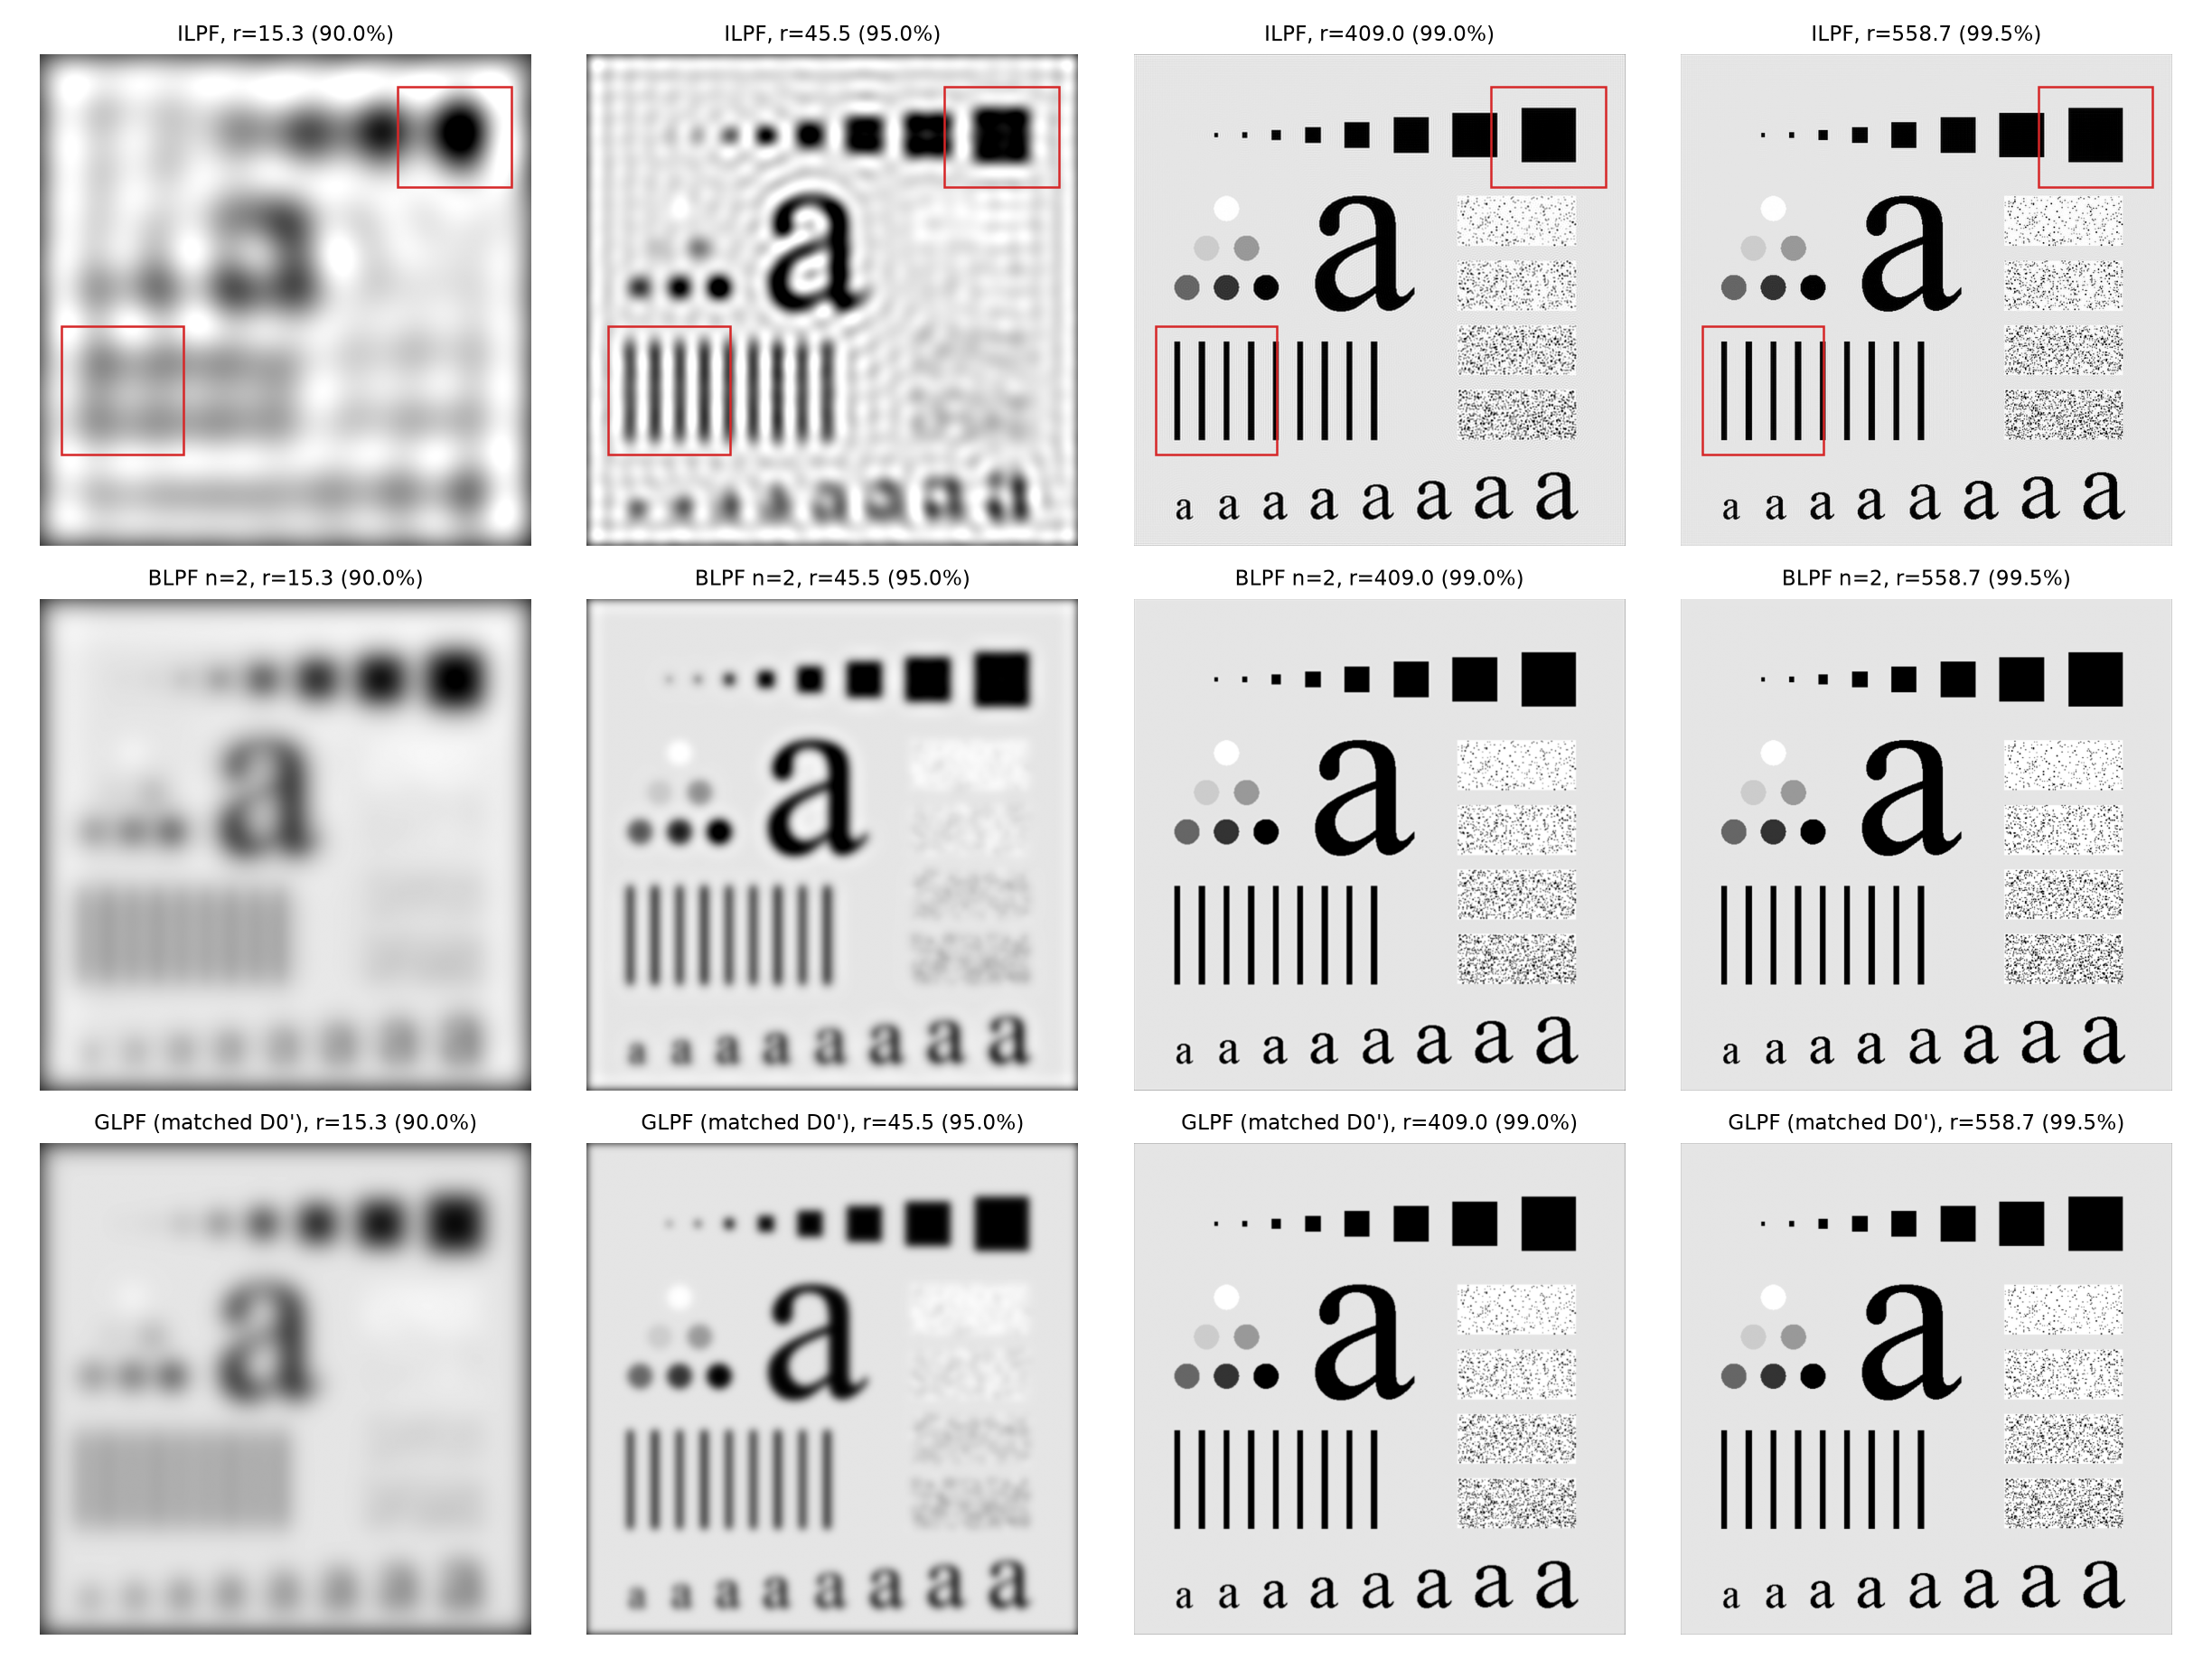
\includegraphics[width=\linewidth]{problem_2/filter_grid.png}
\caption{Rows: ILPF, BLPF $n=2$ and GLPF with the matched $D_0'$. Columns: the
radii that hold 90, 95, 99 and 99.5\,\% of the power. Red boxes mark the insets
of Fig.~\ref{fig:insets}.}
\label{fig:grid}
\end{figure}

\begin{figure}[H]
\centering
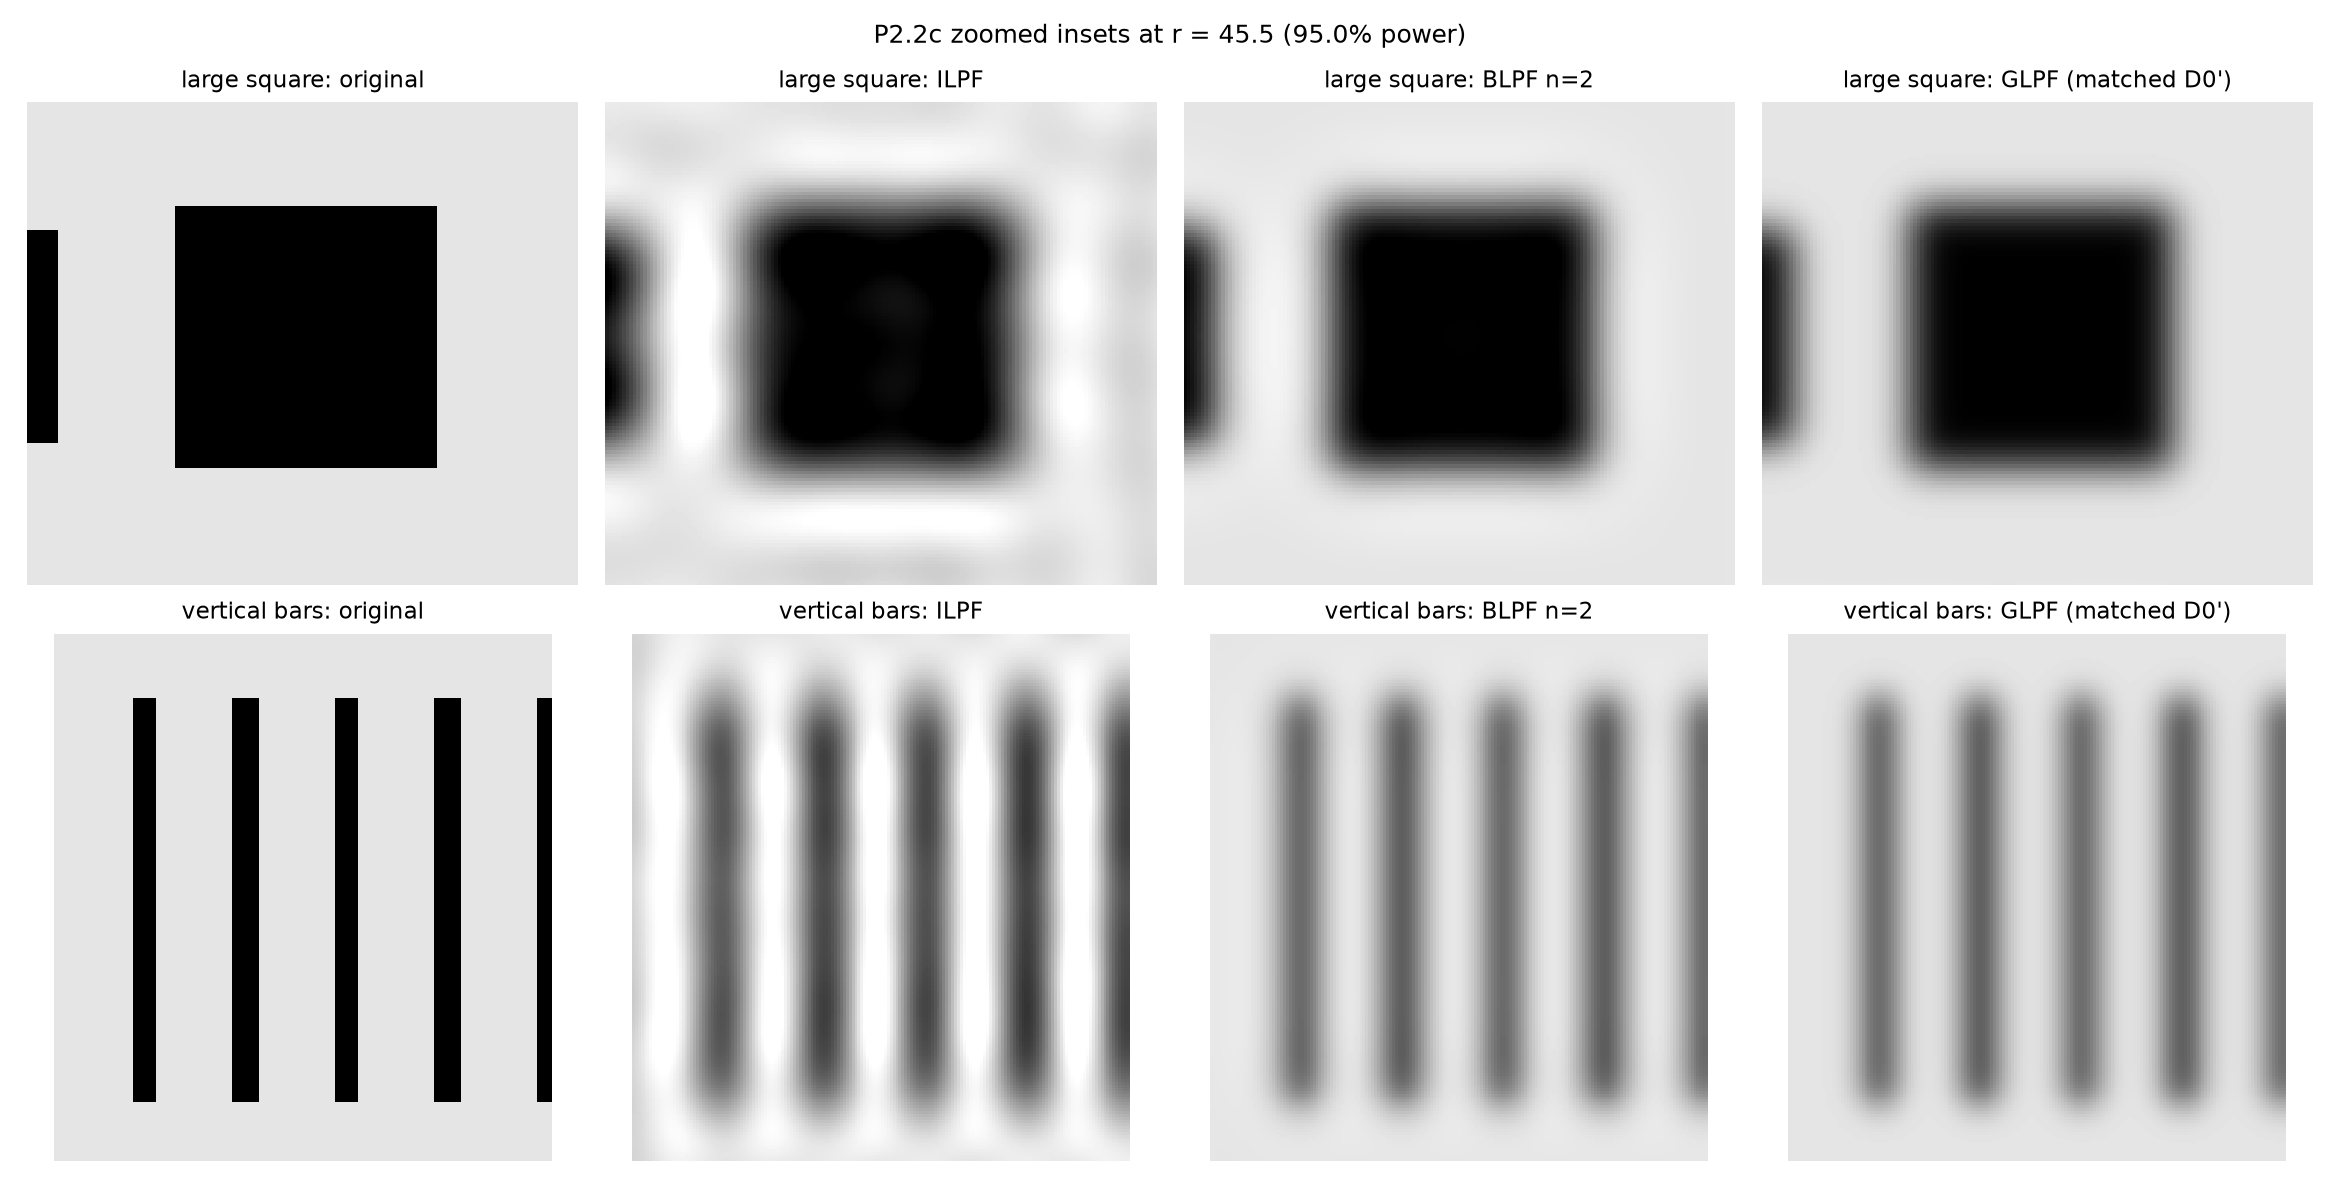
\includegraphics[width=0.9\linewidth]{problem_2/filter_grid_insets.png}
\caption{Ringing in the ideal low-pass output at $r=45.5$: bands beside the large
square and bright gaps between the bars.}
\label{fig:insets}
\end{figure}

\paragraph{(d) Gaussian equivalence.} The Gaussian slice is
$e^{-u^2/2D_0^2}$ with $u$ in bins, i.e.\ frequency $f=u/P$ cycles/pixel. A
spatial Gaussian of standard deviation $\sigma_s$ pixels has the transform
$e^{-2\pi^2\sigma_s^2f^2}=e^{-2\pi^2\sigma_s^2u^2/P^2}$. The two are equal when
$2\pi^2\sigma_s^2/P^2=1/(2D_0^2)$, so
\begin{equation}
\sigma_s=\frac{P}{2\pi D_0}.
\end{equation}
With $P=1376$ this is 21.90, 5.47 and 1.37 pixels for $D_0=10$, 40 and 160. I
ran SciPy's \code{gaussian\_filter} with this $\sigma_s$ and
\code{mode="constant"}, so its boundary matches the zero padding. This is the
comparison the handout asks for and the only place SciPy filters anything.

\begin{table}[H]
\centering
\begin{tabular}{rrrrrr}
\toprule
$D_0$ & $\sigma_s$ (px) & $H$ at $D=P/2$ & max error, truncate 4 & max error, truncate 8 & mean error, truncate 8\\
\midrule
10 & 21.8997 & 0 & $1.571\times10^{-2}$ & $6.253\times10^{-13}$ & $1.813\times10^{-13}$\\
40 & 5.4749 & $5.74\times10^{-65}$ & $1.766\times10^{-2}$ & $3.126\times10^{-13}$ & $5.015\times10^{-14}$\\
160 & 1.3687 & $9.66\times10^{-5}$ & $1.861\times10^{-2}$ & $3.306\times10^{-3}$ & $1.618\times10^{-4}$\\
\bottomrule
\end{tabular}
\caption{$\max|g_\text{freq}-g_\text{spatial}|$ in grey levels on the
characters pattern.}
\label{tab:gauss-eq}
\end{table}

There are two separate reasons the error is not zero. With SciPy's default
\code{truncate=4} the spatial kernel is cut at $4\sigma_s$ and renormalised,
which costs about $2\times10^{-2}$ grey levels at every $D_0$. With the kernel
extended to $8\sigma_s$, the agreement at $D_0=10$ and 40 is rounding, which
confirms the formula for $\sigma_s$. At $D_0=160$ an error of
$3.3\times10^{-3}$ is left, and this part grows with $D_0$ because of sampling.
The frequency-domain filter is a Gaussian that is cut off at the edge of the
$P\times P$ grid, where $H$ is still $9.7\times10^{-5}$. The spatial filter is a
Gaussian sampled at integer pixels, and the spectrum of a sampled function is
the continuous spectrum repeated at every integer frequency. When
$\sigma_s=1.37$ the kernel is barely two pixels wide, its spectrum is wide, the
repeated copies overlap near the Nyquist frequency, and the sharp edges of the
pattern have plenty of energy there. For wide spatial Gaussians (small $D_0$)
both effects disappear.

\subsection{Applications}

\paragraph{(a) Noise and blur.} I added zero-mean Gaussian noise with standard
deviation 20 (seed 2026, not clipped before filtering) to
\code{cameraman.tif}, which gives 22.459 dB. I swept each family over
$D_0=5,\dots,150$ in steps of 1, with $D_0$ the half-amplitude radius (the
Gaussian built with $D_0'$), and clipped the outputs to $[0,255]$ before
computing PSNR.

\begin{table}[H]
\centering
\begin{tabular}{lrrrrrr}
\toprule
Filter & best $D_0$ (5 to 150) & PSNR & best $D_0$ (all) & PSNR & PSNR, $D_0=30$ & PSNR, $D_0=100$\\
\midrule
ILPF & 150 & 27.491 & 215 & 28.690 & 19.723 & 24.940\\
BLPF $n=2$ & 150 & 28.735 & 210 & 29.719 & 20.418 & 26.219\\
GLPF (matched) & 150 & 28.517 & 215 & 29.558 & 20.324 & 26.107\\
\bottomrule
\end{tabular}
\caption{Low-pass denoising of \code{cameraman.tif}, $\sigma=20$, $P=1024$.
PSNR in dB, $D_0$ in bins.}
\label{tab:psnr-sweep}
\end{table}

\begin{figure}[H]
\centering
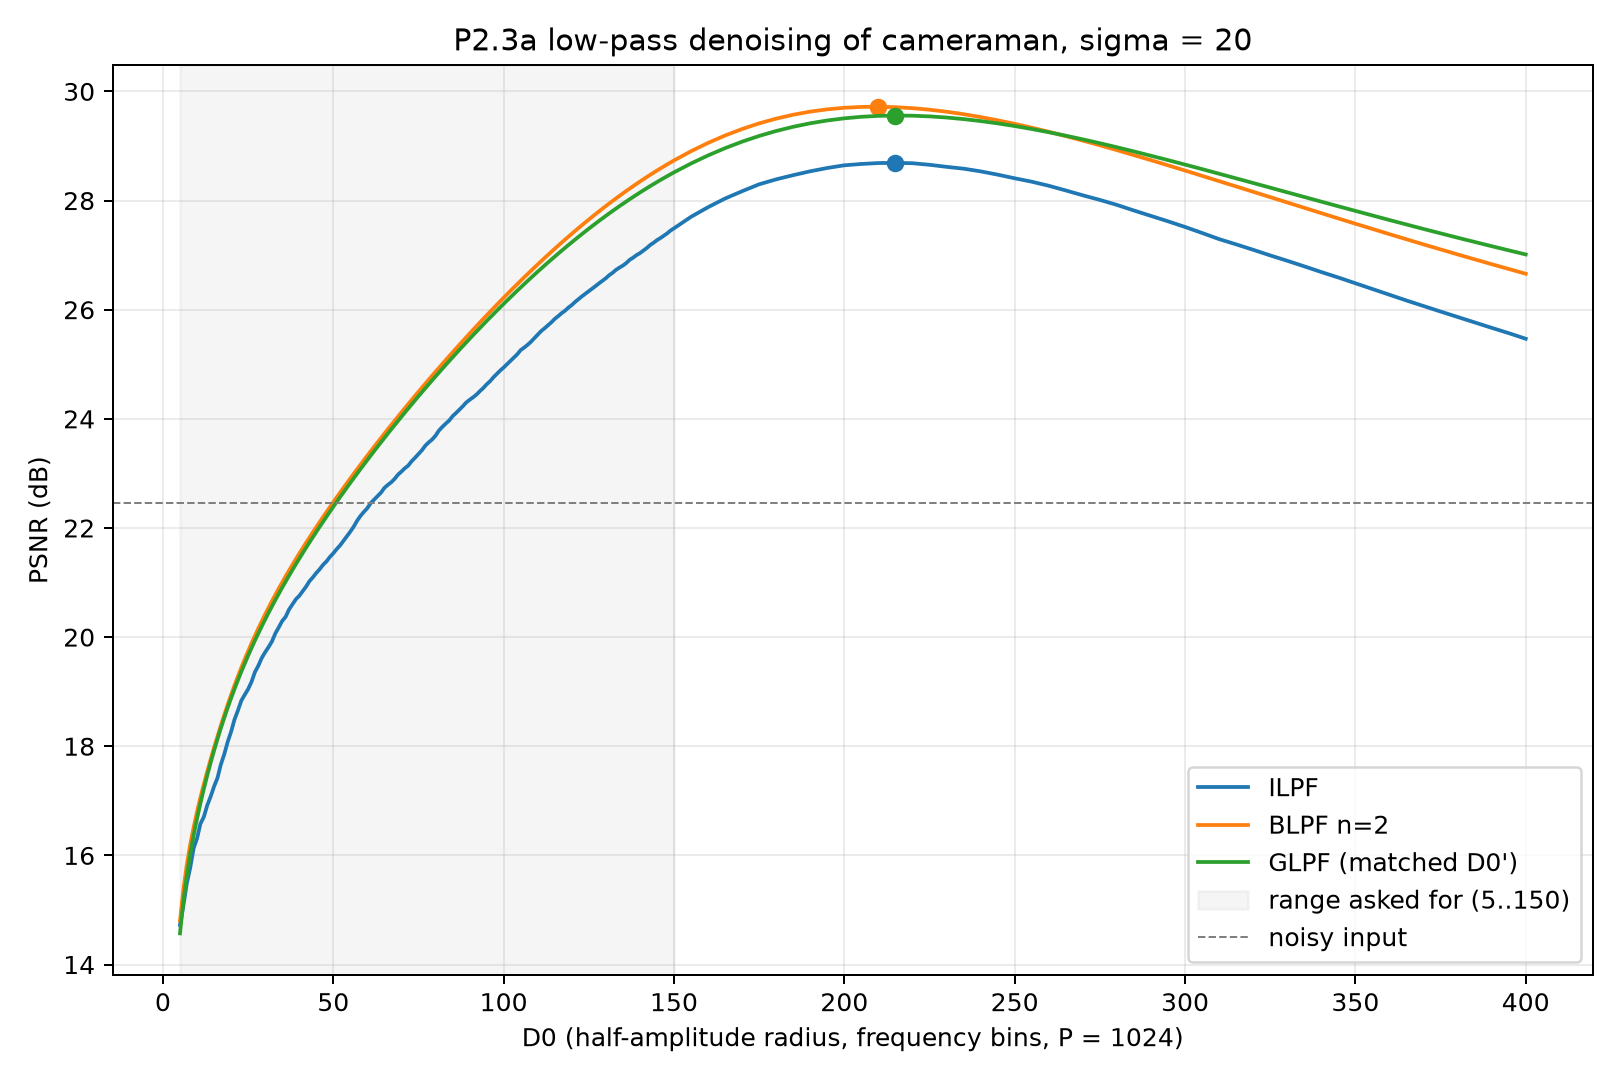
\includegraphics[width=0.7\linewidth]{problem_2/psnr_sweep.png}
\caption{PSNR (dB) against $D_0$ (bins on the $P=1024$ grid). The shaded band
is the range the handout asks for; I extended the sweep to 400 to find the
peaks.}
\label{fig:psnr-sweep}
\end{figure}

Inside the requested range all three curves are still rising at $D_0=150$, so
150 is the edge of the sweep and not an optimum. Extending the sweep in steps of
5 puts the real optima at 210 to 215. This is because of the padded grid:
$D_0=210$ on $P=1024$ is 0.205 cycles/pixel, the same frequency as
$D_0\approx105$ on the unpadded 512-point grid, where the optimum would fall
inside 5 to 150.

The curves peak where they do because white noise has the same power at every
frequency while the image's power falls steeply with frequency. Raising $D_0$
lets through more image detail but also more noise, and the best radius is
roughly where the image spectrum sinks to the noise level. The ideal filter has
the lowest peak (28.69 dB against 29.72 and 29.56 dB), and both reasons can be
read off its transfer function in Fig.~\ref{fig:tf}. It passes noise at full
gain right up to $D_0$ and removes all detail beyond it, whereas the smooth
filters let the noisy band fade out gradually. And its sinc kernel adds ringing
around every edge, which is extra error. The best Butterworth and Gaussian
results differ by only 0.16 dB, since at a matched half-amplitude radius their
transfer functions only differ in how steep the roll-off is. The best outputs
are in \code{psnr\_sweep\_best.png}.

\paragraph{(b) Character repair.} The text has 17766 dark pixels, and a
$3\times3$ morphological closing bridges 3602 gap pixels. I use those gap pixels
as a measurable stand-in for the broken strokes. Table~\ref{tab:text} gives, for
each Gaussian $D_0$, how dark the gaps become relative to the strokes
(``join''), how much darker the strokes stay than the background
(``contrast''), and how many 8-connected pieces are left after thresholding
halfway between the stroke and background levels. The pieces are counted with
my own union-find labelling (\code{label\_components} in
\code{src/common/metrics.py}), which the unit tests check against
\code{scipy.ndimage.label}.

\begin{table}[H]
\centering
\begin{tabular}{rrrrrr}
\toprule
$D_0$ & stroke & gap & join & contrast & pieces\\
\midrule
original & 1.000 & 0.000 & 0.000 & 1.000 & 266\\
40 & 0.292 & 0.273 & 0.933 & 0.274 & 43\\
60 & 0.364 & 0.342 & 0.940 & 0.357 & 102\\
70 & 0.399 & 0.371 & 0.930 & 0.396 & 169\\
\textbf{80} & \textbf{0.433} & \textbf{0.396} & \textbf{0.913} & \textbf{0.431} & \textbf{191}\\
90 & 0.465 & 0.415 & 0.893 & 0.464 & 196\\
120 & 0.548 & 0.448 & 0.819 & 0.548 & 201\\
200 & 0.698 & 0.417 & 0.598 & 0.698 & 208\\
\bottomrule
\end{tabular}
\caption{Gaussian repair of \code{text\_gaps}, $P=1016$ (selected rows of
\code{text\_repair.txt}). Stroke, gap and contrast are darkness
$(255-g)/255$.}
\label{tab:text}
\end{table}

I chose $D_0$ with a written rule: the gaps must be at least 90\,\% as dark as
the strokes, and at most 10\,\% of the pieces may be lost to letters merging,
compared with the least blurred setting (208 pieces at $D_0=200$). I wrote the
rule after a first look at this table, so it states my visual choice precisely
rather than being independent of it. Only $D_0=80$ meets both conditions. Below
it, letters start to fuse (169 pieces at 70, 43 at 40); above it, the gaps stay
visibly lighter than the strokes. In Fig.~\ref{fig:text} the strokes are joined
and the text reads easily.

An ideal filter with the same half-amplitude radius ($80\sqrt{2\ln2}=94.19$)
joins the gaps even more strongly (join 0.977), but its sinc kernel rings. The
output ranges from 37.9 to 317.6 on a 0 to 255 image, every character gets
light and dark halos, and the halos link neighbouring letters, so only 83
pieces are left.

\begin{figure}[H]
\centering
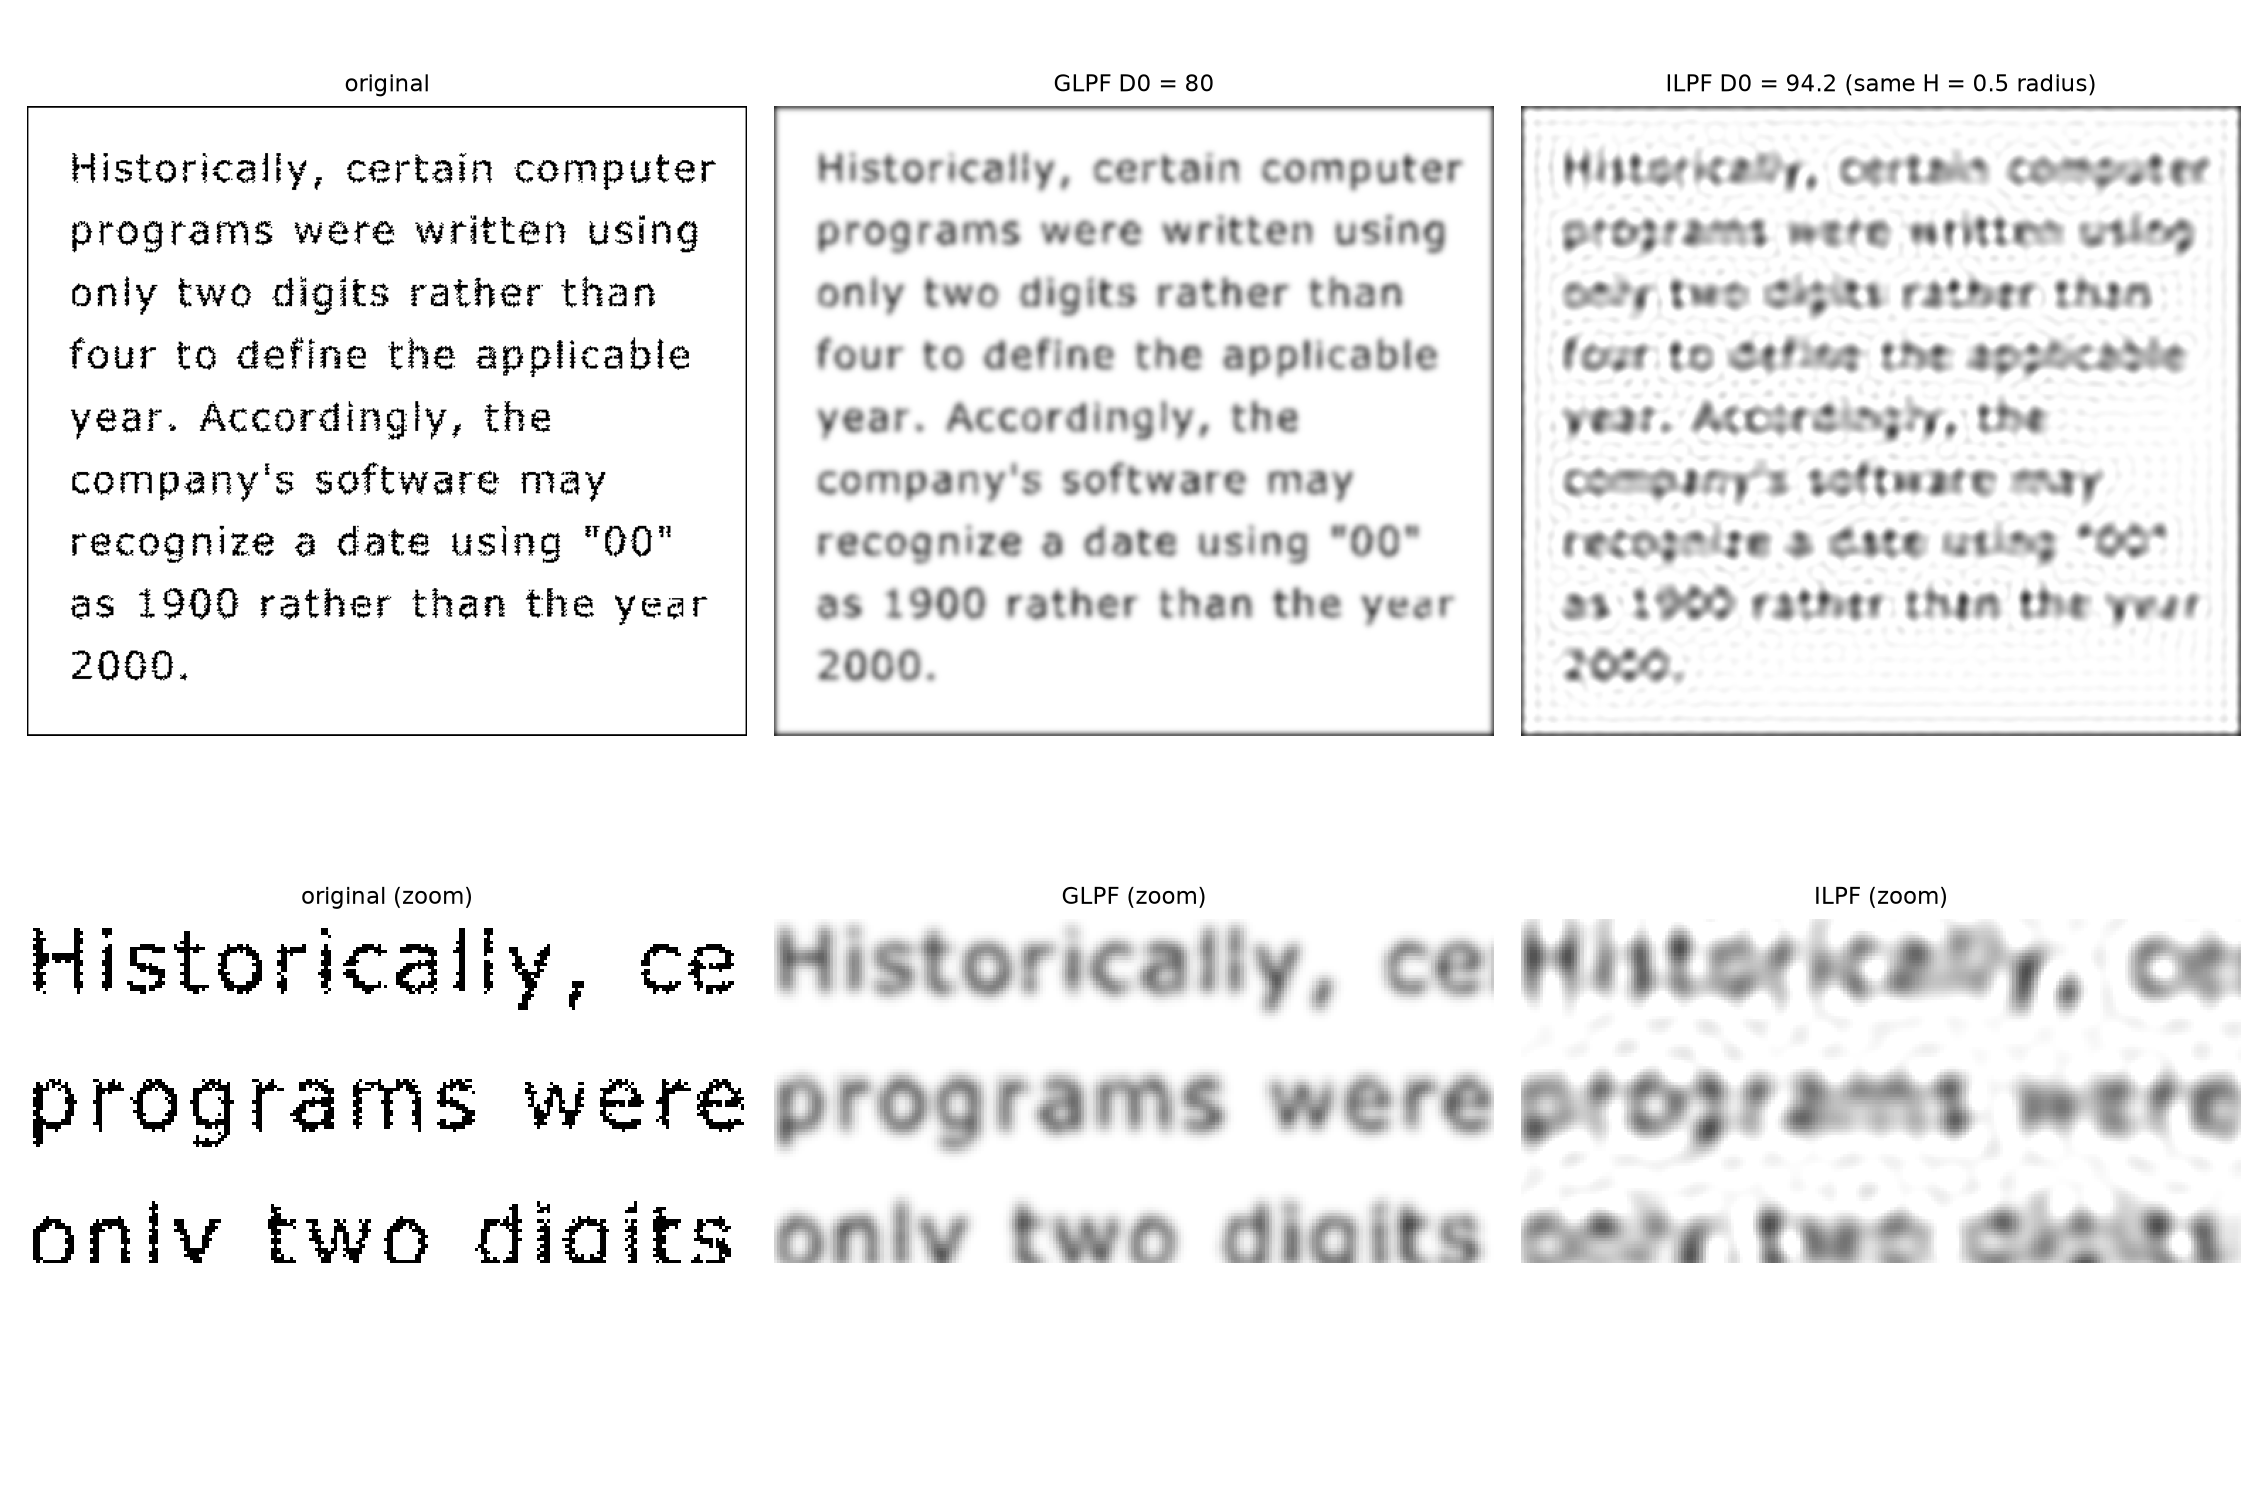
\includegraphics[width=0.85\linewidth]{problem_2/text_repair.png}
\caption{Original, Gaussian $D_0=80$, and the ideal filter with the same
half-amplitude radius, with zoomed crops below.}
\label{fig:text}
\end{figure}

\paragraph{(c) High-pass, DC and emphasis.} I filtered \code{thumb\_print.tif}
with IHPF, BHPF $n=4$ and GHPF at a common half-amplitude radius of 50
($P=2052$).

\begin{table}[H]
\centering
\begin{tabular}{lrrrrrr}
\toprule
Filter & $H_\text{HP}(P/2,P/2)$ & mean (crop) & mean ($P\times P$) & std & pieces $>0$ & specks $<20$ px\\
\midrule
IHPF & 0 & 1.4226 & $8.29\times10^{-17}$ & 32.032 & 840 & 767\\
BHPF $n=4$ & 0 & 1.4588 & $4.15\times10^{-17}$ & 31.486 & 868 & 790\\
GHPF & 0 & 2.0654 & $5.53\times10^{-17}$ & 30.400 & 1088 & 991\\
\bottomrule
\end{tabular}
\caption{High-pass outputs (input mean 142.728). ``Pieces'' and ``specks''
count the 8-connected regions of the ridge map $g>0$.}
\label{tab:hp}
\end{table}

All three filters have $H_\text{HP}(P/2,P/2)=1-H_\text{LP}(0)=0$. The centre
bin is the DC term, which equals $P^2$ times the mean, so the filter removes it
and the mean of the full padded output is zero up to rounding. The mean over the
cropped image is not exactly zero (1.4 to 2.1) because the zero-mean property
holds for the whole $P\times P$ array, and the filtered jump from the image to
the zero padding leaves negative values outside the crop. Compared with the
input mean of 142.7, the tonal information is gone, which is why the high-pass
images look mid-grey.

High-frequency emphasis $H_\text{HFE}=k_1+k_2H_\text{HP}$ with $k_1=0.5$ and
$k_2=0.75$ (Gaussian $H_\text{HP}$) keeps half of the DC and low frequencies and
multiplies the high frequencies by $k_1+k_2=1.25$. Ridges therefore gain a
factor of 2.5 relative to the slow shading, while the tones survive. The output
mean is 72.913, close to $k_1\cdot142.728=71.364$ (the rest is again the crop
effect). The overall spread stays the same as the input's (standard deviation
40.455 against 40.427), but it is redistributed: the shading across the print is
halved and the ridges are sharper (Fig.~\ref{fig:hp}).

Thresholding each high-pass output at zero gives a ridge map. By the number of
small specks, the ideal (767) and Butterworth (790) maps are about equally clean
and the Gaussian map is clearly the noisiest (991). At a common half-amplitude
radius the Gaussian high-pass rises slowly: at $D=25$ it already passes 16\,\%
of the low frequencies, against 0.4\,\% for Butterworth $n=4$ and 0 for the
ideal filter. That leaked shading moves the zero crossings and breaks ridges
into fragments. The ideal and Butterworth maps both show a dark band along the
top border, where the print meets the zero padding and the filter responds to
that artificial edge. Butterworth $n=4$ has almost the steep roll-off of the
ideal filter without its sinc kernel, so it is the safer choice, although on this
image the speck count does not separate the two.

\begin{figure}[H]
\centering
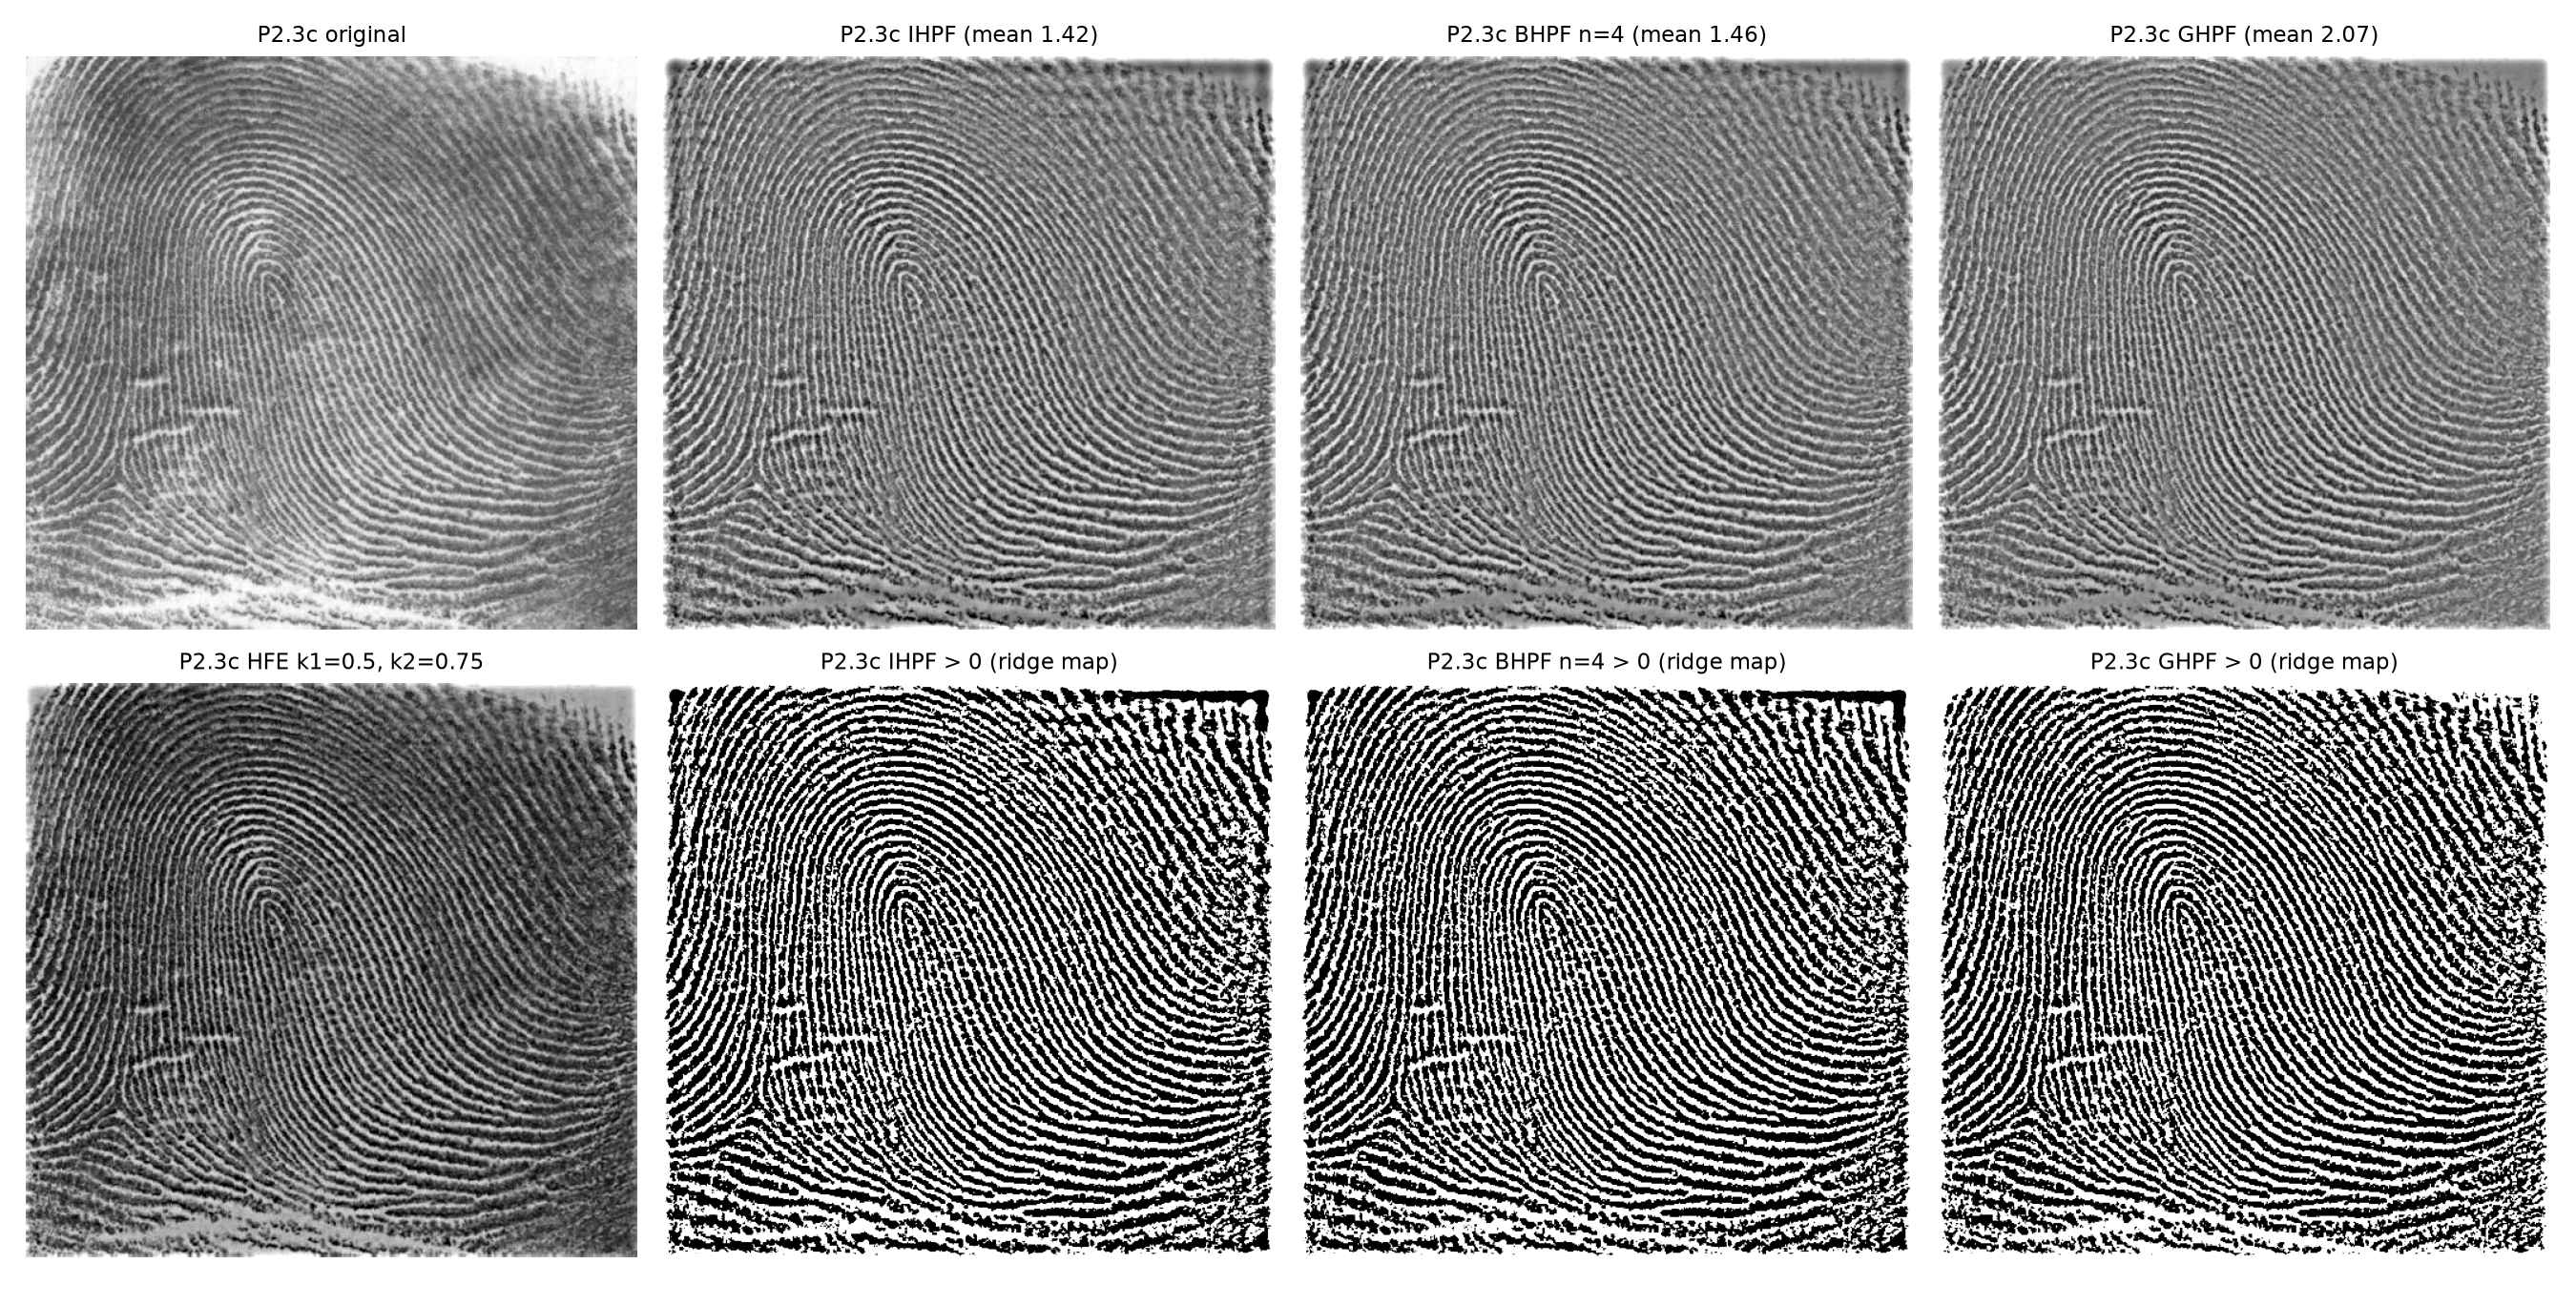
\includegraphics[width=\linewidth]{problem_2/highpass.png}
\caption{High-pass outputs (on a symmetric grey range), high-frequency emphasis,
and the ridge maps from thresholding at zero.}
\label{fig:hp}
\end{figure}

\section{Homomorphic filtering: illumination and reflectance}

\textbf{Data.} \code{tunnel\_image.jpg} ($3644\times3000$, a phone photograph looking
along a dark tunnel towards a bright opening) is unevenly lit in exactly the way
the problem describes: deep shadow on the walls and floor and a bright, clipped
region at the far end. It was converted to luminance
$Y=0.299R+0.587G+0.114B$ in $[0,1]$ and box-averaged $4\times4$ to $911\times750$,
which keeps every structure of interest and makes a full parameter sweep quick.

\subsection{The multiplicative model}

Following the standard homomorphic model \cite{gonzalez}, the image is modelled as $I(x,y)=L(x,y)R(x,y)$, with illumination $L>0$ varying
slowly across the scene and reflectance $R\in(0,1]$ carrying edges and texture. A
linear filter cannot separate the two directly, because the Fourier transform of a
product is a convolution, $\mathcal{F}\{I\}=\mathcal{F}\{L\}\circledast\mathcal{F}\{R\}$:
every reflectance frequency is smeared by the illumination spectrum, so no
frequency band belongs to $L$ or to $R$ alone. Taking the logarithm first turns the
product into a sum,
\begin{equation}
z=\ln I=\ln L+\ln R,\qquad Z=\mathcal{F}\{z\}=\mathcal{F}\{\ln L\}+\mathcal{F}\{\ln R\},
\end{equation}
and the Fourier transform keeps that sum because it is linear. Since $\ln L$ is
smooth, its spectrum sits near the origin, while $\ln R$ has most of its energy at
higher frequencies. A filter $H$ with gain $\gamma_L<1$ near the origin and
$\gamma_H>1$ further out then acts on each part separately, and exponentiating
gives approximately
\begin{equation}
\hat I=\exp\big(\mathcal{F}^{-1}\{HZ\}\big)\approx L^{\gamma_L}R^{\gamma_H},
\end{equation}
which compresses the illumination range and stretches the reflectance contrast.

The log must come before the transform. The point of the log is to make the
spatial product additive, and it does so only when applied to the pixel values.
After the transform the product has already become a convolution, and the log of a
convolution is not a sum of anything useful. Filtering the log-magnitude spectrum
instead, $\log|G|=H\log|\mathcal{F}\{I\}|$, i.e.\ $|G|=|\mathcal{F}\{I\}|^{H}$ with the
original phase, is a fixed power law on spectral magnitudes. It is the same
operation for every pixel, so it cannot brighten dark regions more than lit ones,
and the phase is left paired with magnitudes it no longer belongs to.

A synthetic check makes this quantitative. With a Gaussian light $L$ from 0.03 to 1
and a block texture $R\in\{0.4,0.9\}$, the reflectance detail (mean $9\times9$ local
standard deviation) is 22.7 times larger in the lit region than in the dark one,
because the detail is scaled by $L$. Table~\ref{tab:logcheck} applies the same
$H$ ($D_0=20$, $\gamma_L=0.5$, $\gamma_H=1.5$) three ways.

\begin{table}[H]
\centering
\begin{tabular}{lrrr}
\toprule
Method & detail, lit & detail, dark & lit / dark\\
\midrule
input $I=LR$ & 0.2212 & 0.0097 & 22.69\\
filter $I$ directly & 0.3313 & 0.0146 & 22.73\\
filter $\log|\mathcal{F}\{I\}|$ & 3.7230 & 0.2250 & 16.55\\
filter $\log I$ (homomorphic) & 0.4468 & 0.0855 & 5.23\\
\bottomrule
\end{tabular}
\caption{Detail in lit ($L>0.9$) and dark ($L<0.06$) regions of the synthetic
scene (\code{log\_domain\_check.txt}).}
\label{tab:logcheck}
\end{table}

Filtering $I$ directly scales all detail by the same factor and leaves the ratio at
22.7. Filtering the log-magnitude spectrum changes it only to 16.6 and inflates the
values tenfold. The homomorphic filter brings the ratio to 5.23, close to the
$22.69^{\gamma_L}=4.76$ that $\hat I\approx L^{\gamma_L}R^{\gamma_H}$ predicts. It
is a little higher because the separation by frequency is not perfect: the block
texture has some low-frequency energy, which receives $\gamma_L$ rather than
$\gamma_H$.

\subsection{Implementation and tuning}

\code{homomorphic} in \code{src/problem\_3/homomorphic.py} computes
$z=\ln(I+1/255)$ (the offset keeps black pixels finite), mirror-pads $z$ to
$P=2\max(\text{rows},\text{cols})=1822$, multiplies the centred spectrum by
\begin{equation}
H(u,v)=(\gamma_H-\gamma_L)\big[1-e^{-cD^2(u,v)/D_0^2}\big]+\gamma_L,\qquad c=1,
\end{equation}
inverts, crops, and returns $e^{z'}-1/255$. Mirror padding replaces the zero
padding of Problem 2 here: zero is a very negative value in the log domain, and
zero padding would put a large artificial step at every border. To compare methods
on equal terms, every output, the input included, is mapped to $[0,1]$ by its own
0.1 and 99.9 percentiles.

The measurements use two regions defined from the input: the shadow is the darkest
25\,\% of the $31\times31$ smoothed luminance (170813 pixels: floor, lower walls,
corners), and the bright region is the top 1\,\% (6833 pixels: the opening).
Shadow and bright contrast are the mean $15\times15$ local standard deviation in
those regions, ``bright sat.'' is the share of bright pixels at or above 0.98,
``levels'' counts distinct 8-bit output values in the shadow, and ``reversal''
measures halos. It is the share of the strongest 25\,\% of input gradients, both
images smoothed with a $15\times15$ box, whose direction the output reverses. A
global monotone tone curve cannot reverse a smoothed gradient, so this is close to
zero for histogram equalisation; a halo is precisely a band beside a large edge
where the output slopes the wrong way.

\begin{table}[H]
\centering
\small
\begin{tabular}{rrrrrrrrrr}
\toprule
$D_0$ & $\gamma_L$ & $\gamma_H$ & shadow contr. & bright contr. & bright sat. & blown out & levels & shadow mean & reversal\\
\midrule
\multicolumn{3}{l}{input} & 0.0015 & 0.0033 & 1.000 & 0.0116 & 7 & 0.0110 & 0.0000\\
\midrule
10 & 0.25 & 1.25 & 0.0142 & 0.0157 & 0.076 & 0.0030 & 87 & 0.2347 & 0.0872\\
10 & 0.25 & 2.00 & 0.0157 & 0.0237 & 0.012 & 0.0021 & 87 & 0.2175 & 0.1094\\
10 & 0.50 & 1.50 & 0.0074 & 0.0149 & 0.101 & 0.0030 & 41 & 0.1010 & 0.0495\\
10 & 0.75 & 1.25 & 0.0034 & 0.0085 & 0.313 & 0.0050 & 15 & 0.0306 & 0.0083\\
40 & 0.25 & 1.25 & 0.0186 & 0.0082 & 0.000 & 0.0024 & 102 & 0.3087 & 0.0966\\
40 & 0.25 & 2.00 & 0.0224 & 0.0111 & 0.000 & 0.0014 & 110 & 0.3185 & 0.1323\\
40 & 0.50 & 1.50 & 0.0096 & 0.0076 & 0.071 & 0.0035 & 47 & 0.1305 & 0.0531\\
40 & 0.50 & 2.00 & 0.0117 & 0.0106 & 0.001 & 0.0024 & 55 & 0.1536 & 0.0773\\
40 & 0.75 & 1.25 & 0.0039 & 0.0047 & 0.475 & 0.0070 & 16 & 0.0342 & 0.0085\\
160 & 0.25 & 1.25 & 0.0195 & 0.0032 & 0.006 & 0.0025 & 85 & 0.2420 & 0.0226\\
160 & 0.25 & 2.00 & 0.0261 & 0.0045 & 0.000 & 0.0017 & 111 & 0.3109 & 0.0470\\
160 & 0.50 & 1.50 & 0.0094 & 0.0032 & 0.991 & 0.0127 & 37 & 0.0915 & 0.0058\\
\textbf{160} & \textbf{0.50} & \textbf{2.00} & \textbf{0.0117} & \textbf{0.0040} & \textbf{0.012} & \textbf{0.0023} & \textbf{46} & \textbf{0.1205} & \textbf{0.0137}\\
160 & 0.75 & 1.25 & 0.0037 & 0.0030 & 1.000 & 0.0121 & 13 & 0.0233 & 0.0002\\
160 & 0.75 & 2.00 & 0.0054 & 0.0039 & 0.989 & 0.0123 & 20 & 0.0458 & 0.0035\\
\bottomrule
\end{tabular}
\caption{Selected rows of the 27-setting sweep (all rows in
\code{sweep\_metrics.txt}). Bold: the setting chosen as good.}
\label{tab:sweep}
\end{table}

\begin{figure}[H]
\centering
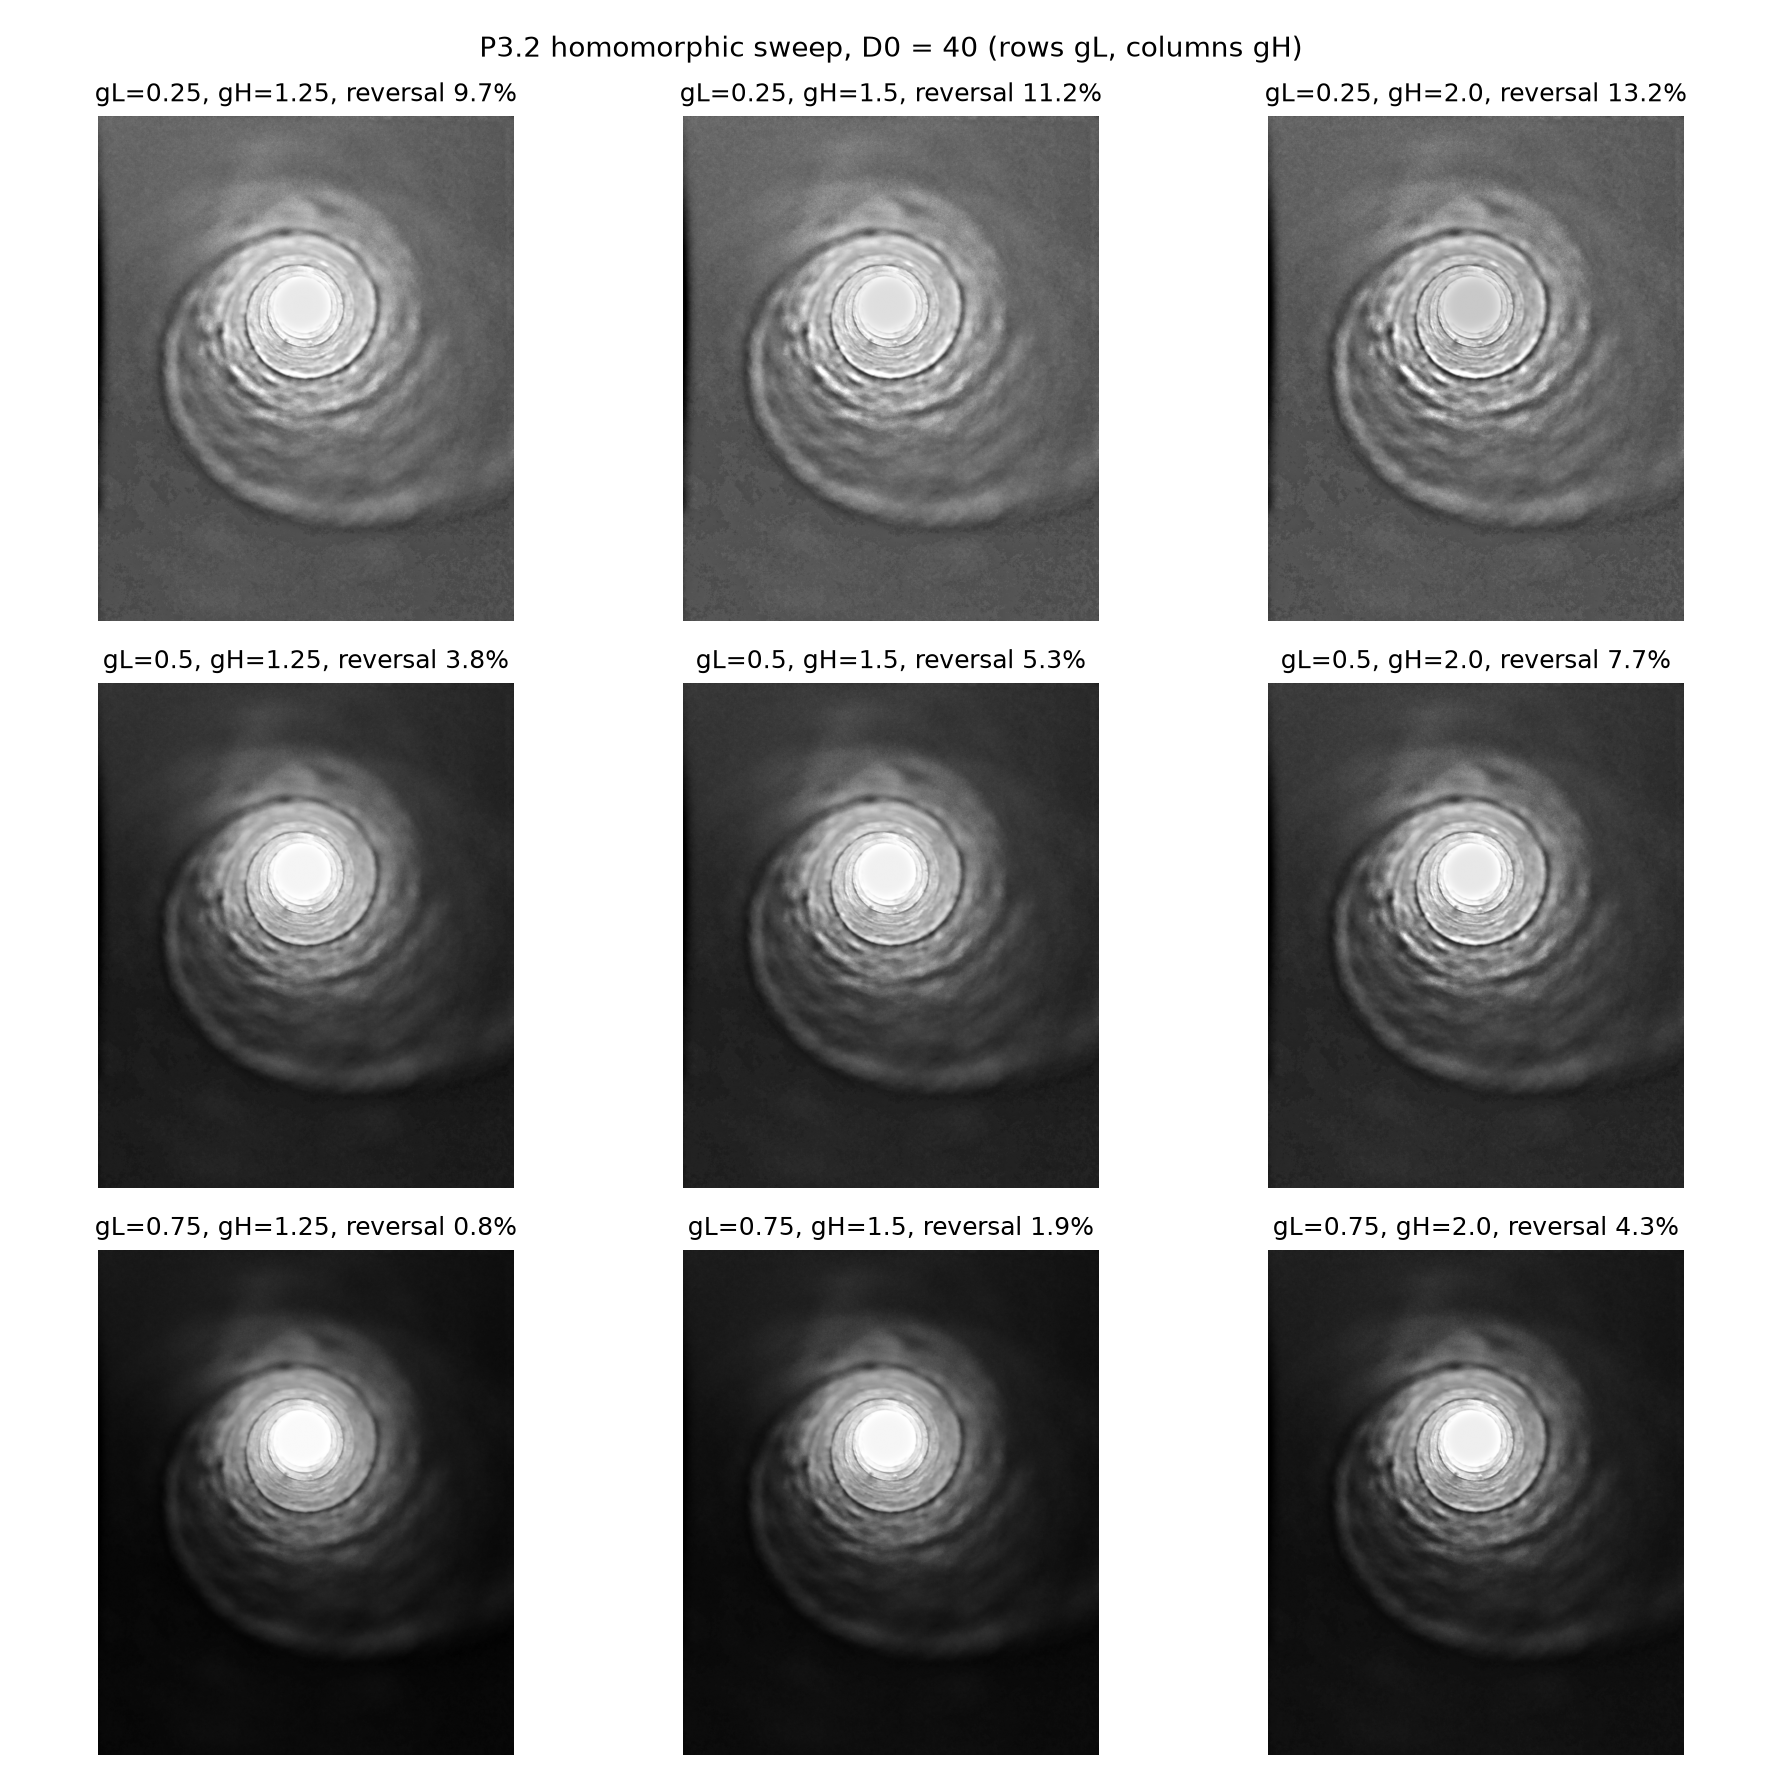
\includegraphics[width=0.49\linewidth]{problem_3/sweep_grid_d0_40.png}
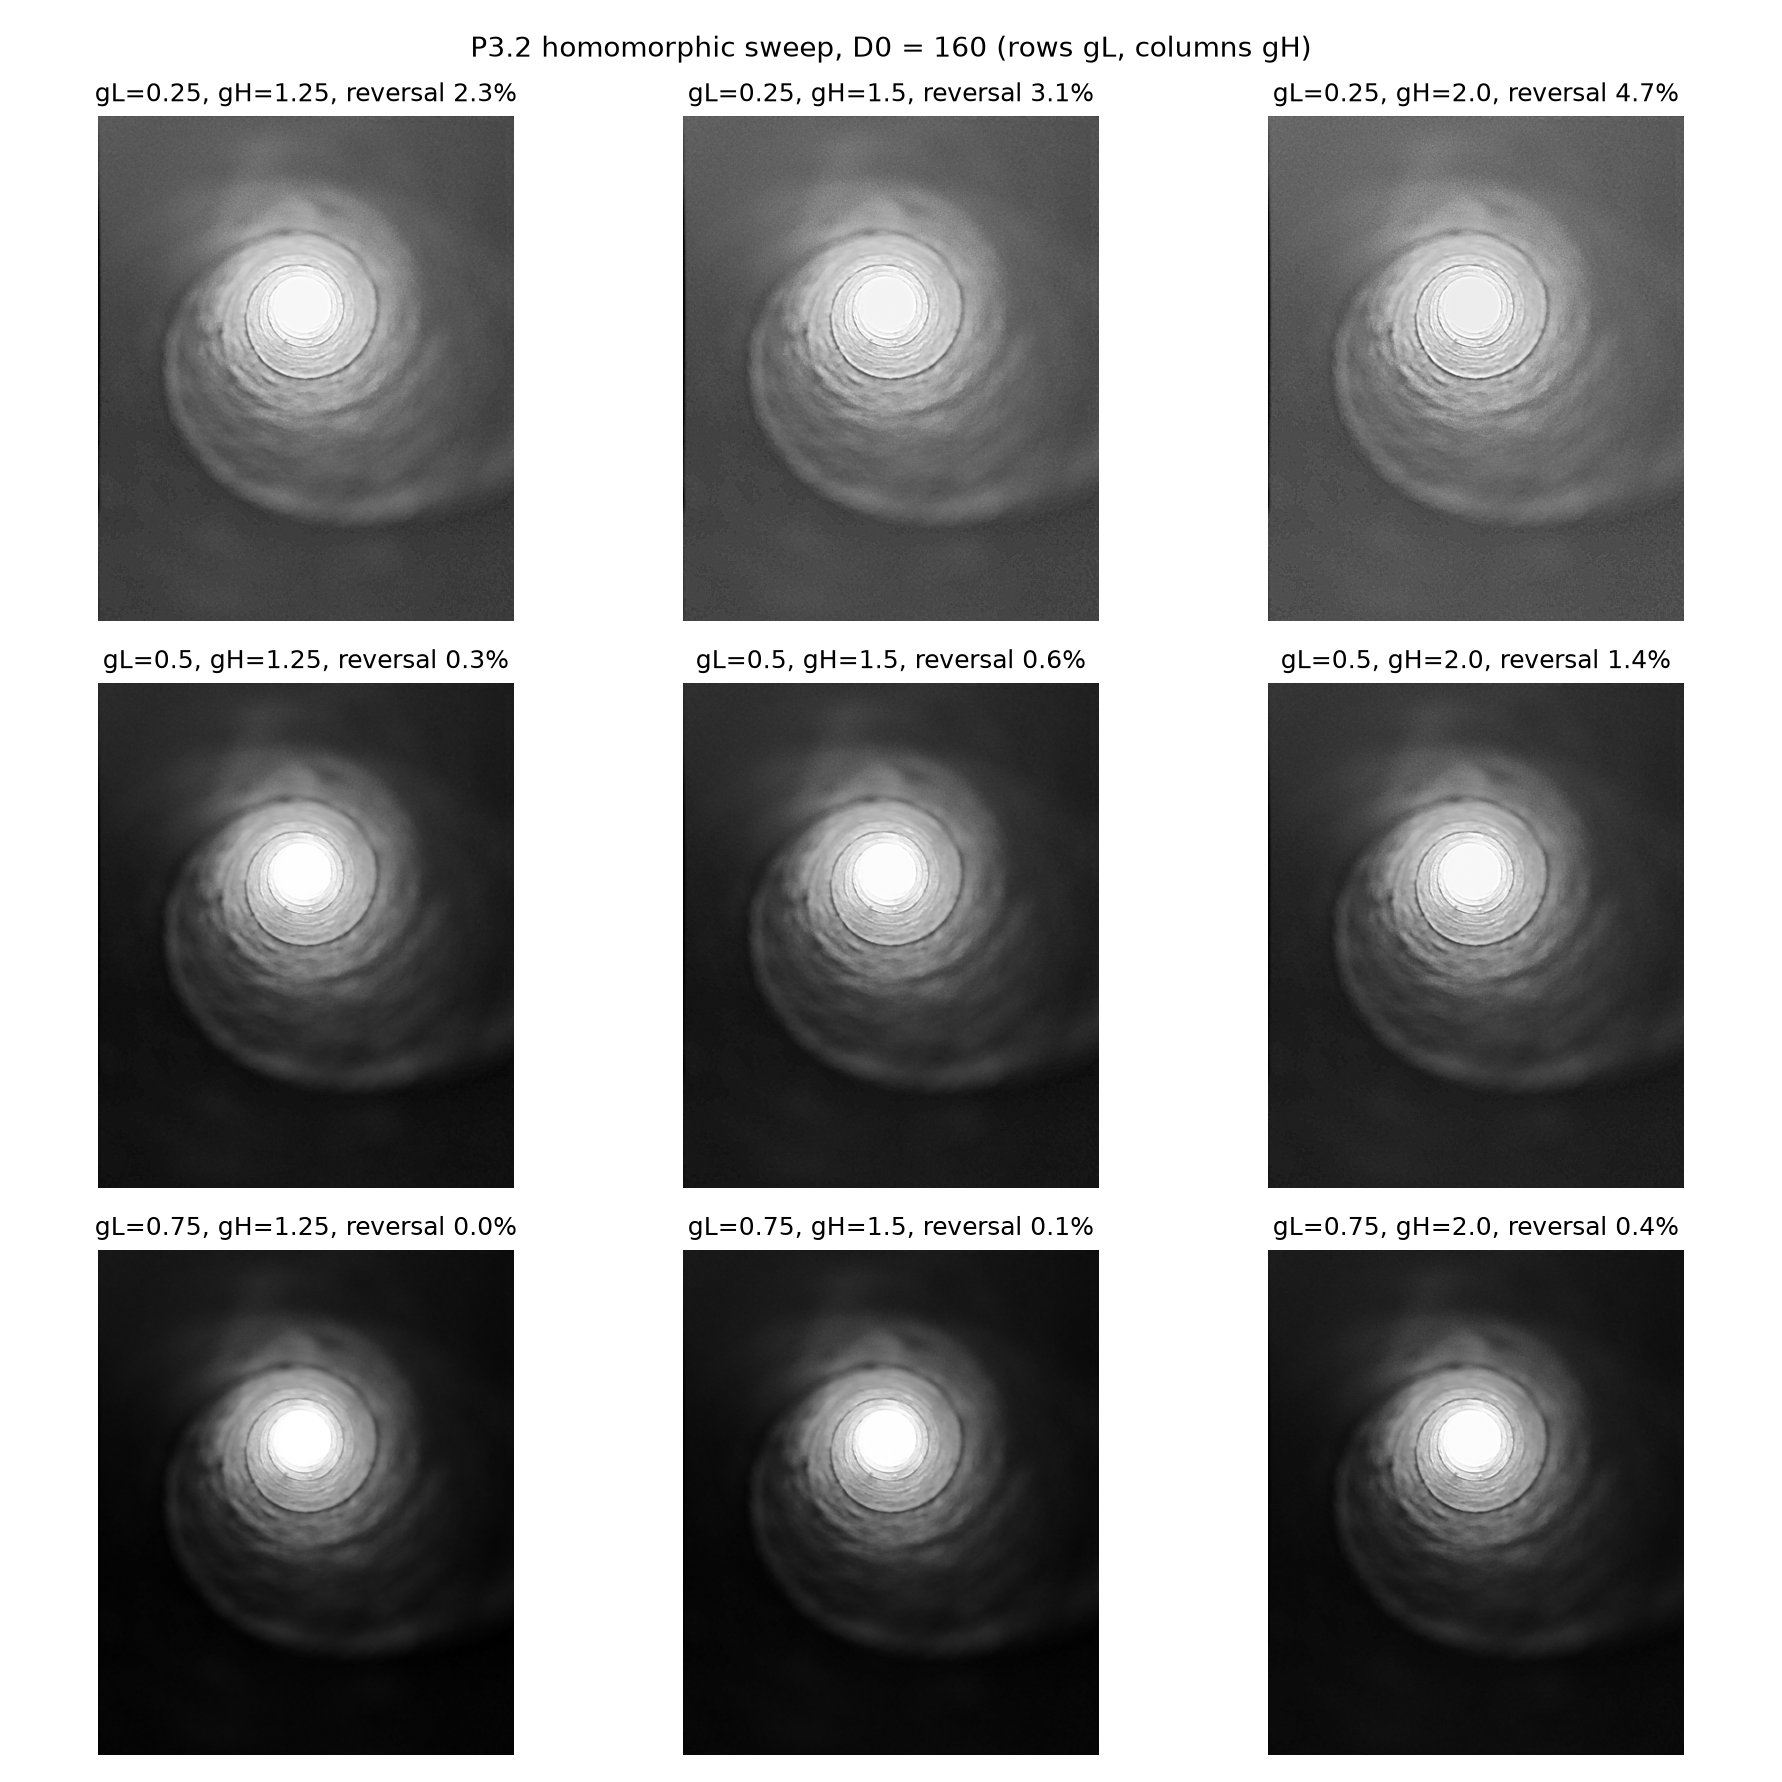
\includegraphics[width=0.49\linewidth]{problem_3/sweep_grid_d0_160.png}
\caption{Sweep grids for $D_0=40$ (left) and $D_0=160$ (right): rows
$\gamma_L=0.25,0.5,0.75$, columns $\gamma_H=1.25,1.5,2$. The $D_0=10$ grid is in
\code{sweep\_grid\_d0\_10.png}.}
\label{fig:sweep}
\end{figure}

The parameters act as the model says. $\gamma_L$ sets how much the illumination is
flattened: going from 0.75 to 0.25 lifts the mean shadow level from 0.02--0.07 to
0.22--0.32 at every $D_0$. $\gamma_H$ sets the detail gain, and the contrast in both
regions rises with it. $D_0$ sets the scale that counts as illumination. The
low-pass part $e^{-D^2/D_0^2}$ is a Gaussian with spatial standard deviation
$\sigma=\sqrt2\,P/(2\pi D_0)$, i.e.\ 41, 10 and 2.6 pixels for $D_0=10$, 40 and 160.

\textbf{Halos} appear where strong flattening ($\gamma_L=0.25$) meets strong
emphasis ($\gamma_H=2$), and they are worst at $D_0=40$: reversal 13.2\,\% at
$(40,0.25,2)$, against 10.9\,\% at $D_0=10$ and 4.7\,\% at $D_0=160$. The filter
behaves like unsharp masking in the log domain, and every large edge gets an over-
and undershoot band about $\sigma$ wide. At $D_0=40$ the bands are about 10 pixels
wide, the same scale as the rings of the tunnel and the rim of the opening, so they
read as bright and dark contours; Fig.~\ref{fig:sweep} (left, top row) shows
them around the light. At $D_0=160$ they are too thin to be visible as halos, and at
$D_0=10$ they are broad and gentle.

\textbf{Good settings.} No setting stays below 1\,\% reversal without leaving the
light saturated, so the rule was set at reversal $\le2\,\%$ and bright saturation
$\le10\,\%$, then the largest shadow contrast. Like the rule in 2.3b, these limits
were chosen after seeing the table. The rule selects $(D_0,\gamma_L,\gamma_H)=(160,0.5,2)$:
shadow contrast 7.8 times the input's, mean shadow level up from 0.0110 to 0.1205,
1.2\,\% of the light saturated, and 1.4\,\% gradient reversal.

One caution about the bright region: 98.3\,\% of its full-resolution pixels have at
least one channel at 255, so the light is clipped in the JPEG itself. A setting that
lowers ``bright sat.'' maps that flat clipped area below white; it does not recover
detail that was never recorded. Indeed, at $D_0=160$ with $\gamma_H\le1.5$ the light
stays saturated, while $\gamma_H=2$ creates small overshoots at its rim that take
the top percentile and push the flat interior below 0.98.

\subsection{Comparison with histogram equalisation}

Global histogram equalisation uses the Assignment 1 implementation,
$T(v)=\operatorname{round}(255F(v))$ on the 8-bit luminance, with $F$ the inclusive
cumulative histogram.

\begin{table}[H]
\centering
\small
\begin{tabular}{lrrrrrrr}
\toprule
Method & shadow contr. & bright contr. & bright sat. & blown out & levels & shadow mean & reversal\\
\midrule
input & 0.0015 & 0.0033 & 1.000 & 0.0116 & 7 & 0.0110 & 0.0000\\
histogram equalisation & 0.0321 & 0.0015 & 1.000 & 0.0218 & 7 & 0.1670 & 0.0005\\
homomorphic $(160,0.5,2)$, good & 0.0117 & 0.0040 & 0.012 & 0.0023 & 46 & 0.1205 & 0.0137\\
homomorphic $(40,0.25,2)$, halo & 0.0224 & 0.0111 & 0.000 & 0.0014 & 110 & 0.3185 & 0.1323\\
\bottomrule
\end{tabular}
\caption{Local contrast and side effects (\code{local\_contrast.txt}).}
\label{tab:he}
\end{table}

\begin{figure}[H]
\centering
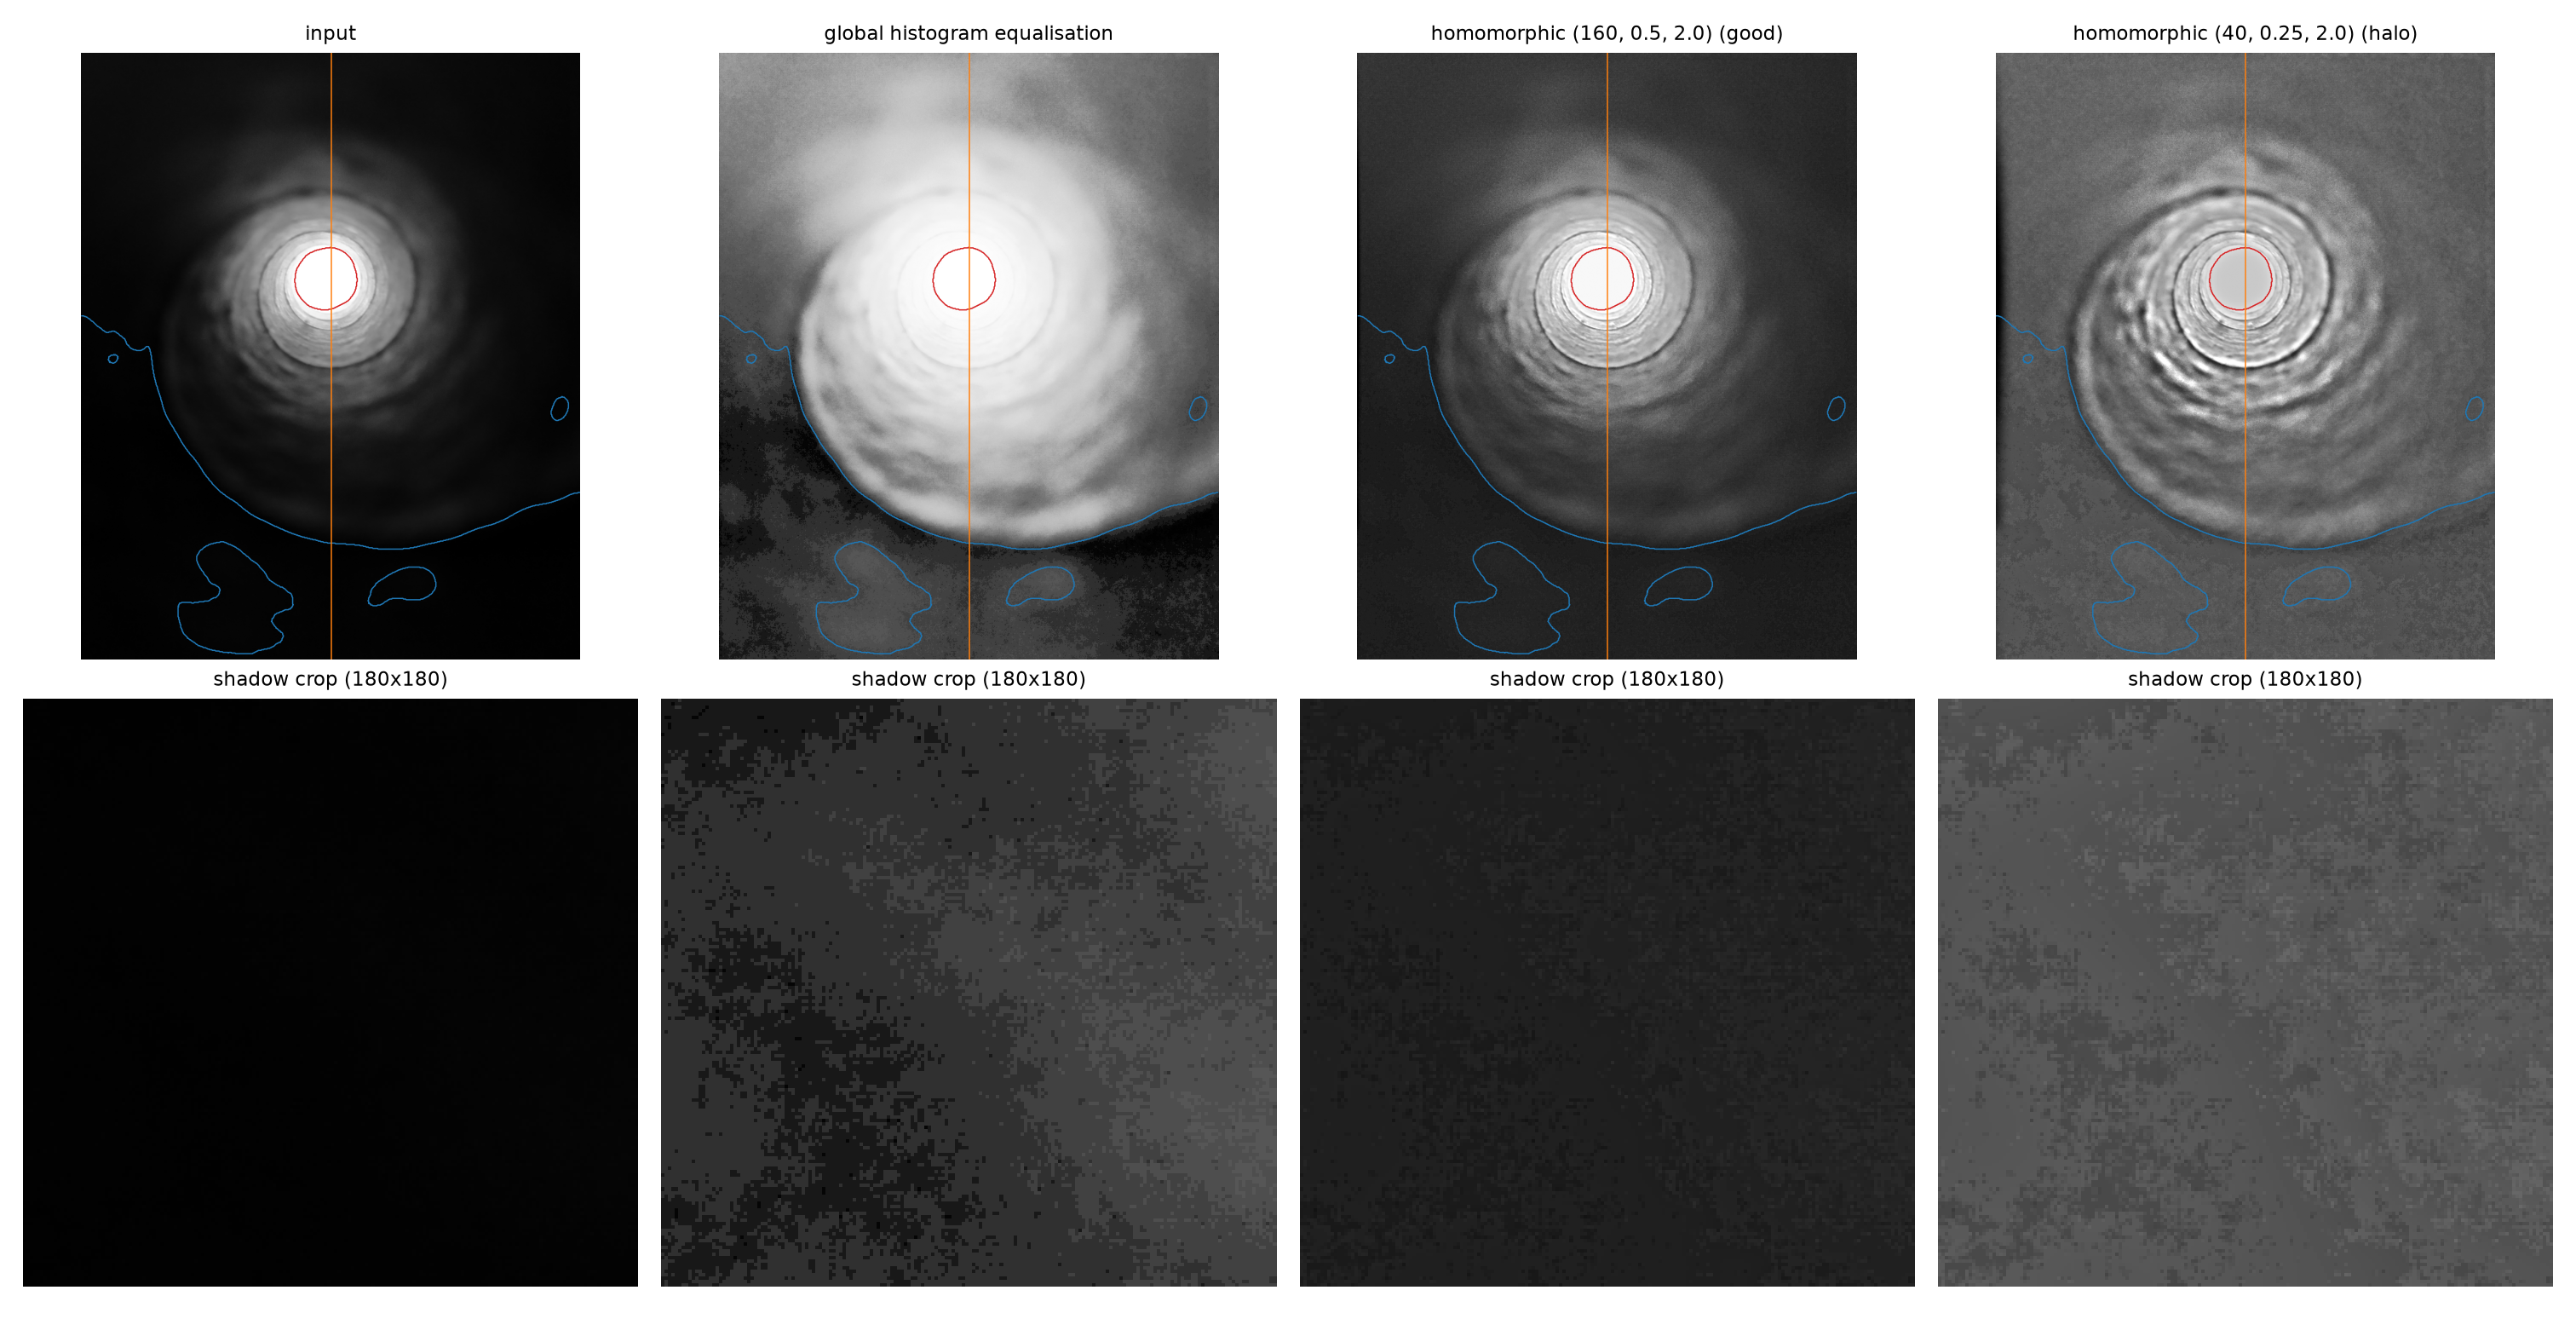
\includegraphics[width=\linewidth]{problem_3/homomorphic_comparison.png}
\caption{Input, equalisation and two homomorphic settings, with the shadow region
(blue) and bright region (red) outlined and a $180\times180$ shadow crop below.}
\label{fig:homo}
\end{figure}

\begin{figure}[H]
\centering
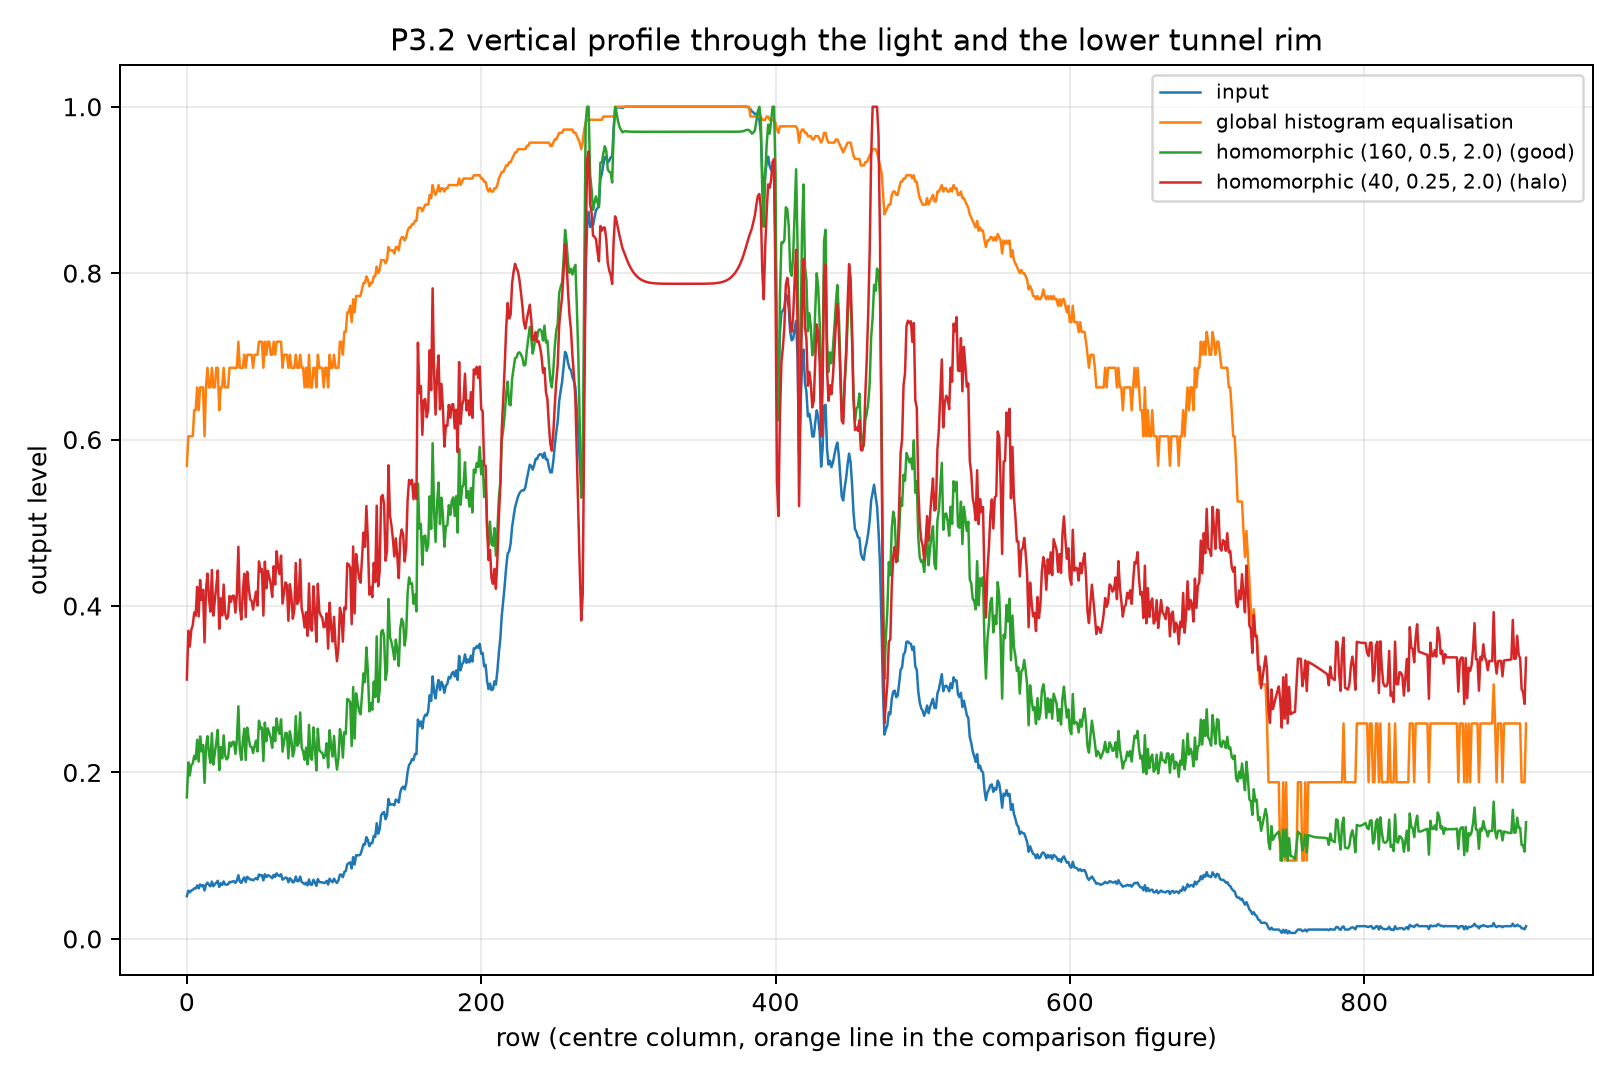
\includegraphics[width=0.75\linewidth]{problem_3/profiles.png}
\caption{Vertical profile through the centre column (orange line in
Fig.~\ref{fig:homo}).}
\label{fig:homo-profile}
\end{figure}

By raw local standard deviation, equalisation wins in the shadow (0.0321 against
0.0117), but that number is not recovered detail. The shadow of the input occupies
only seven distinct 8-bit values, and a look-up table cannot create new ones, so
equalisation spreads those seven values far apart. Its shadow ``contrast'' is the
quantisation steps and sensor noise made visible as blotchy posterisation
(Fig.~\ref{fig:homo}, shadow crop; the staircase in Fig.~\ref{fig:homo-profile}).
It also pushes most of the lit tunnel wall towards white (blown-out share up from
1.16\,\% to 2.18\,\%), and the light remains fully saturated. Equalisation allocates
output range by pixel counts over the whole image and has no notion of what is
illumination and what is reflectance.

The good homomorphic setting lifts the shadow by a factor of about 11 in mean level
and 7.8 in local contrast, renders it with 46 distinct levels instead of 7 (each
output pixel depends on its neighbourhood, so the filter interpolates between the
quantised input values), keeps the lit walls away from white (0.23\,\% blown out)
and has no visible halos. It therefore recovers shadow detail better without
blowing out the bright region. The reason is the one in 3.1: it compresses $L$ and
keeps $R$, so contrast in the dark is raised by the same factor as the
illumination is lowered. Two limits remain. Detail that the 8-bit file never
recorded cannot be recovered by either method, and pushing for more shadow
contrast with $\gamma_L=0.25$ produces the halos of the $(40,0.25,2)$ setting, whose
profile maps the clipped light to a flat plateau at 0.79 with spikes to 1.0 at its
rim (Fig.~\ref{fig:homo-profile}).

\paragraph{Conclusion.} The log turns $I=LR$ into a sum that a linear filter can
split by frequency, which the synthetic check confirms (detail ratio 22.7 reduced
to 5.2, with 4.8 predicted). On the tunnel image, homomorphic filtering lifts the
shadows without saturating the walls. Strong flattening and emphasis at the scale
of the scene's large structures produces halos, which the gradient-reversal measure
detects.

\section{Edge-preserving smoothing: bilateral and Kuwahara}

\textbf{Data.} The clean ground truth \code{q4.png} ($512\times512$) has a
200-level rectangle and a 20-level disc on a 60-level background, plus a
horizontal ramp from 66 to 103 that overlaps the disc. Its edges therefore range
from 140 levels (rectangle) down to 40 levels (disc against background). The
noisy input adds zero-mean Gaussian noise with $\sigma=20$ (seed 2026), which
gives 22.265 dB.

\subsection{Implementation and matched strength}

\textbf{Bilateral filter} \cite{tomasi} (\code{src/problem\_4/bilateral.py}):
\begin{equation}
g(\mathbf p)=\frac{\sum_{\mathbf q\in\Omega}w(\mathbf p,\mathbf q)f(\mathbf q)}{\sum_{\mathbf q\in\Omega}w(\mathbf p,\mathbf q)},\qquad
w(\mathbf p,\mathbf q)=\exp\!\Big(-\frac{\|\mathbf p-\mathbf q\|^2}{2\sigma_s^2}\Big)\exp\!\Big(-\frac{(f(\mathbf p)-f(\mathbf q))^2}{2\sigma_r^2}\Big),
\end{equation}
over a square window $\Omega$ of radius $r$ with reflected borders. Dividing by
the sum of the weights is the normalisation, so a flat region is left unchanged.
The code loops over the $(2r+1)^2$ window offsets, and each step is one array
operation over the whole image.

\textbf{Classical Kuwahara filter} \cite{kuwahara}
(\code{src/problem\_4/kuwahara.py}): for a window of size $N=2a+1$, I form the
four $(a+1)\times(a+1)$ sub-windows that share the centre row and column, and
output the mean of the one with the smallest variance. The sub-window sums of $f$
and $f^2$ come from two integral images, so the cost per pixel does not depend on
$N$.

\paragraph{(a) Matched smoothing strength.} The two filters have different
parameters, so ``the same amount of smoothing'' has to be defined first. I call
the filters matched when they
\begin{enumerate}
\item use the same footprint: the bilateral window radius equals the Kuwahara
half-width $a$, with $\sigma_s=a/2$ so that the window spans $\pm2\sigma_s$; and
\item reduce noise by the same amount where there is no edge: on a flat field
($256\times256$, value 128, the same $\sigma=20$, seed 11) the variance ratio
$\operatorname{var}(\text{output})/\operatorname{var}(\text{input})$ is the same.
\end{enumerate}
The first condition gives both filters the same neighbourhood to work with. The
second fixes the smoothing in flat regions, which is what ``strength'' means when
there is nothing to preserve. With both fixed, any difference at an edge can only
come from how each filter decides which neighbours to trust. That leaves
$\sigma_r$ as the only free parameter, and I find it by bisection on the variance
ratio.

\begin{table}[H]
\centering
\begin{tabular}{rrrrrr}
\toprule
$N$ & Kuwahara variance ratio & $\sigma_s$ & $\sigma_r$ & bilateral variance ratio & $1/(a+1)^2$\\
\midrule
5 & 0.12859 & 1.00 & 54.191 & 0.12859 & 0.11111\\
7 & 0.06906 & 1.50 & 51.918 & 0.06906 & 0.06250\\
11 & 0.02956 & 2.50 & 57.862 & 0.02956 & 0.02778\\
\bottomrule
\end{tabular}
\caption{Matched parameters (\code{matching.txt}). The matched $\sigma_r$ comes
out at 2.6 to 2.9 times the noise standard deviation.}
\label{tab:match}
\end{table}

The Kuwahara variance ratio is a bit above $1/(a+1)^2$, the variance ratio of a
single sub-window mean. The sub-windows share pixels, and which one gets chosen
depends on the same noise as its mean, so the selected mean is not an
independent average.

\paragraph{(b) Evaluation.}

\begin{table}[H]
\centering
\begin{tabular}{lrrr}
\toprule
Method & PSNR (dB) & SSIM & edge-band RMSE\\
\midrule
noisy input & 22.265 & 0.1674 & 19.506\\
Kuwahara $5\times5$ & 31.031 & 0.6069 & 8.114\\
bilateral $\sigma_s=1$, $\sigma_r=54.2$ & 30.941 & 0.5935 & 8.693\\
Kuwahara $7\times7$ & 33.558 & 0.7497 & 7.220\\
bilateral $\sigma_s=1.5$, $\sigma_r=51.9$ & 33.416 & 0.7384 & 7.823\\
Kuwahara $11\times11$ & 36.662 & 0.8788 & 7.294\\
bilateral $\sigma_s=2.5$, $\sigma_r=57.9$ & 36.139 & 0.8727 & 8.749\\
\bottomrule
\end{tabular}
\caption{Matched pairs against the clean image. Outputs are clipped to
$[0,255]$, data range 255. SSIM is my NumPy implementation of \cite{wang} with a
$7\times7$ uniform window, $K_1=0.01$, $K_2=0.03$ (checked against scikit-image
in the unit tests). The edge band is every pixel within 3 pixels of a
ground-truth jump larger than 5 levels; RMSE in 8-bit levels.}
\label{tab:edge-pres}
\end{table}

At every matched size Kuwahara is slightly ahead in PSNR (0.09 to 0.52 dB) and
SSIM, and clearly ahead near edges: its edge-band RMSE is 7.2 to 8.1 against 7.8
to 8.7. Since flat-region smoothing is equal by construction, the difference
comes from the edges, and the crops in Fig.~\ref{fig:edge-pres} show where. At
the 140-level rectangle edge both filters keep a sharp boundary. At the 40-level
disc edge the bilateral filter has a problem: with $\sigma_r=51.9$ a jump of 40
levels gets range weight $e^{-40^2/(2\cdot51.9^2)}=0.74$, almost as much as a
neighbour on the same side, so it averages across the edge and leaves it soft.
Kuwahara does not compare intensities pixel by pixel. It picks a whole
sub-window, usually one that lies on one side of the edge, so the boundary stays
sharp even at this contrast. With a step of 40 and noise of 20, the extra variance
of a sub-window that straddles the edge (about $p(1-p)\cdot40^2\le400$) is no
larger than the noise variance, so the choice is not always right, which is why
the boundary is slightly ragged. Kuwahara's own artifact shows in the flat areas:
a patchwork of small flat blocks instead of the bilateral filter's smooth
leftover texture.

\begin{figure}[H]
\centering
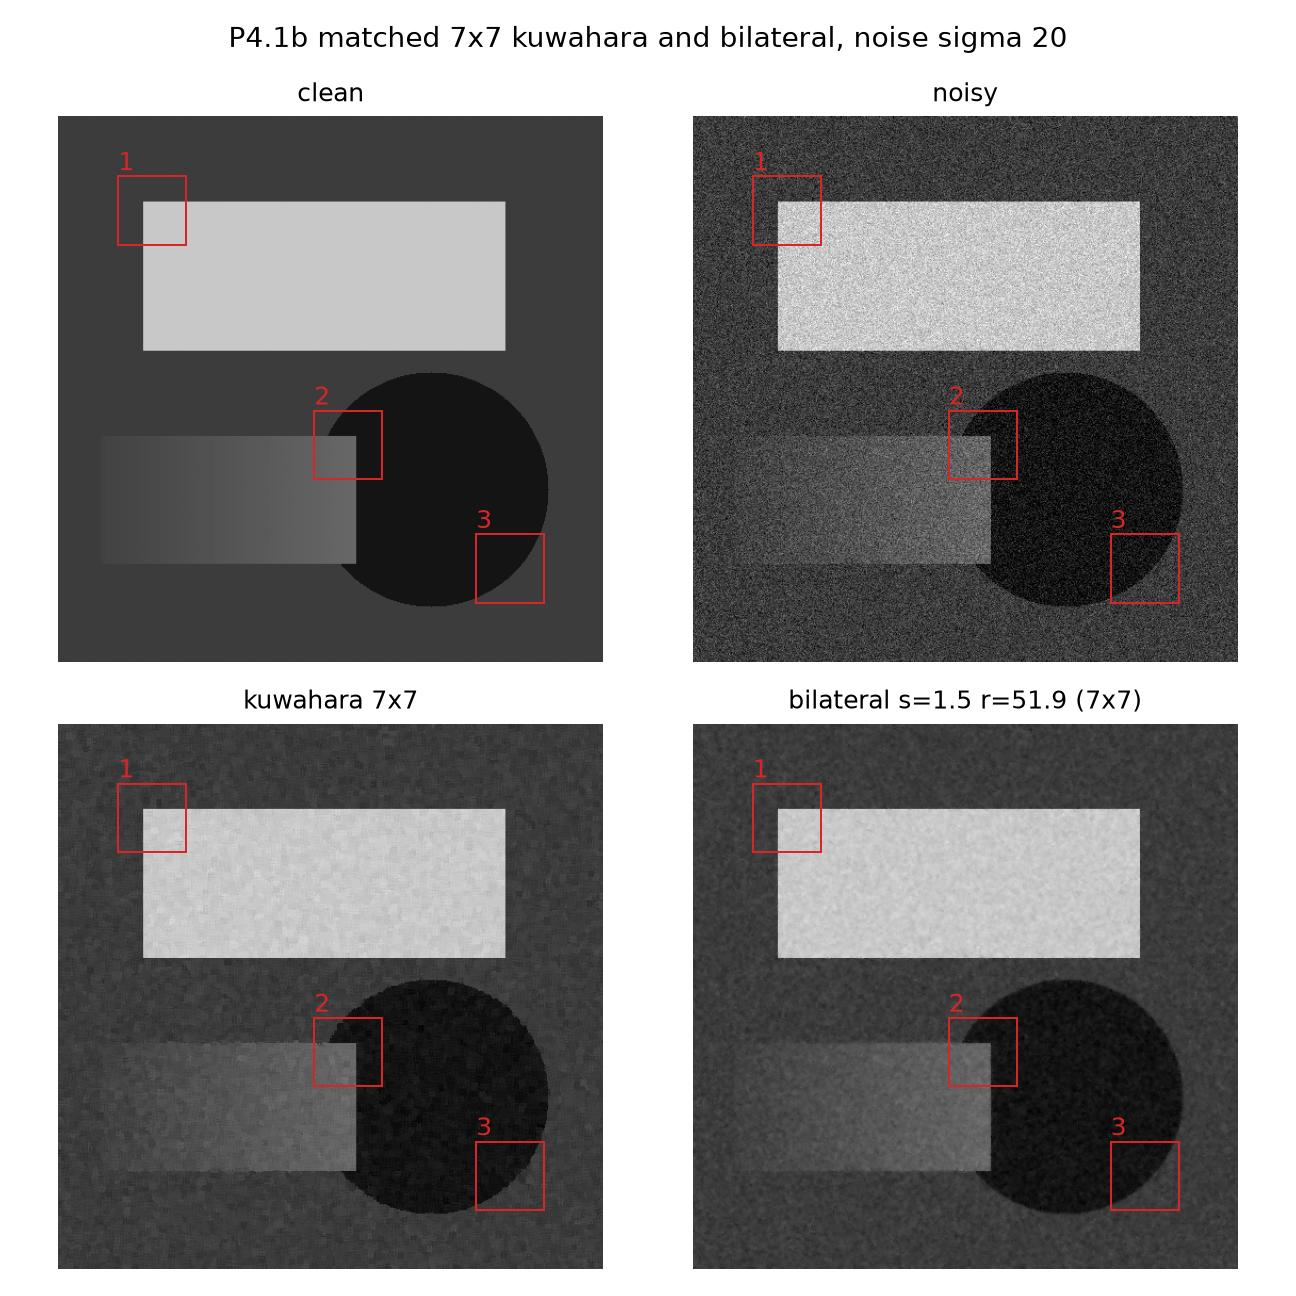
\includegraphics[width=0.92\linewidth]{problem_4/edge_preservation_comparison.png}
\caption{Matched $7\times7$ pair. Rows 2 to 4 are the $64\times64$ crops boxed in
red: the rectangle corner (contrast 140), the ramp crossing the disc, and the
disc edge (contrast 40).}
\label{fig:edge-pres}
\end{figure}

\subsection{Kuwahara blockiness and complexity}

\paragraph{(a) Why the hard argmin makes blocks.} In a flat noisy region, each of
the four sub-window means changes slowly as the window slides, because it is a
moving average. Which of the four has the smallest variance is a discrete choice,
though, and it can flip from one pixel to the next. When it flips, the output
jumps from one sub-window mean to another, a step that is not in the input.
Neighbouring windows share most of their pixels, so the same sub-window tends to
win over a whole patch. The output becomes patches of nearly constant value
separated by small steps, the painterly blocks, and their size grows with the
sub-window. This is not blur, because the chosen sub-window lies on one side of an
edge and never averages across it. It is not ringing either: the output is always
the plain mean of input samples, a weighted average with non-negative weights, so
by the argument in 2.2(b) it stays inside the local range of the input and cannot
overshoot.

\paragraph{(b) Soft Kuwahara.} My modification replaces the argmin with softmax
weights on the negative variances,
\begin{equation}
g=\frac{\sum_{k=1}^4 w_k m_k}{\sum_k w_k},\qquad
w_k=\exp\!\Big(-\frac{s_k^2-\min_j s_j^2}{T}\Big),\qquad T=\sigma^2=400,
\end{equation}
with $m_k$ and $s_k^2$ the sub-window means and variances. Subtracting the
minimum only guards against underflow and cancels in the ratio. The output is now
a continuous function of the variances, so it cannot jump when two of them swap
order. Near a strong edge, a sub-window that straddles it has its variance raised
by about $p(1-p)\Delta I^2$ (4900 for half of a 140-level step), which gives it
weight $e^{-12}$, so it is still left out, as in the classical filter. With
$T=\sigma^2$, two sub-windows whose variances differ by about the noise variance
are blended instead of chosen between. I measure blockiness away from the true
edges (242792 pixels at least 4 pixels from any jump) by the total variation
$\overline{|\partial_xg|+|\partial_yg|}$ and by the 99th percentile of
$|\nabla g|$. Both are tiny on the clean image (0.017 and 1.000).

\begin{table}[H]
\centering
\begin{tabular}{rlrrrrr}
\toprule
$N$ & method & TV & p99 $|\nabla g|$ & PSNR (dB) & SSIM & edge RMSE\\
\midrule
11 & classical & 4.436 & 12.556 & 36.662 & 0.8788 & 7.294\\
11 & soft & 1.751 & 3.477 & 39.866 & 0.9638 & 6.870\\
15 & classical & 2.997 & 9.240 & 38.304 & 0.9270 & 7.679\\
15 & soft & 1.141 & 2.367 & 40.401 & 0.9764 & 7.794\\
\bottomrule
\end{tabular}
\caption{Classical and soft Kuwahara at identical window sizes
(\code{blockiness.txt}). TV and gradients in grey levels per pixel.}
\label{tab:block}
\end{table}

The soft version cuts the total variation by 61\,\% at $N=11$ and 62\,\% at
$N=15$, and the 99th-percentile gradient (the size of the larger block steps) by
72\,\% and 74\,\%. PSNR rises by 3.2 and 2.1 dB. Edge RMSE improves at $N=11$ and
gets slightly worse at $N=15$ (7.79 against 7.68). At the low-contrast disc edge
the variance of a straddling sub-window only rises by about 400, so it keeps
weight $e^{-1}$ and the edge gets mixed a little. Fig.~\ref{fig:block} shows the
ramp, where the classical filter turns a smooth gradient into flat steps and the
soft filter keeps it smooth, and the rectangle corner, which both keep sharp.

\begin{figure}[H]
\centering
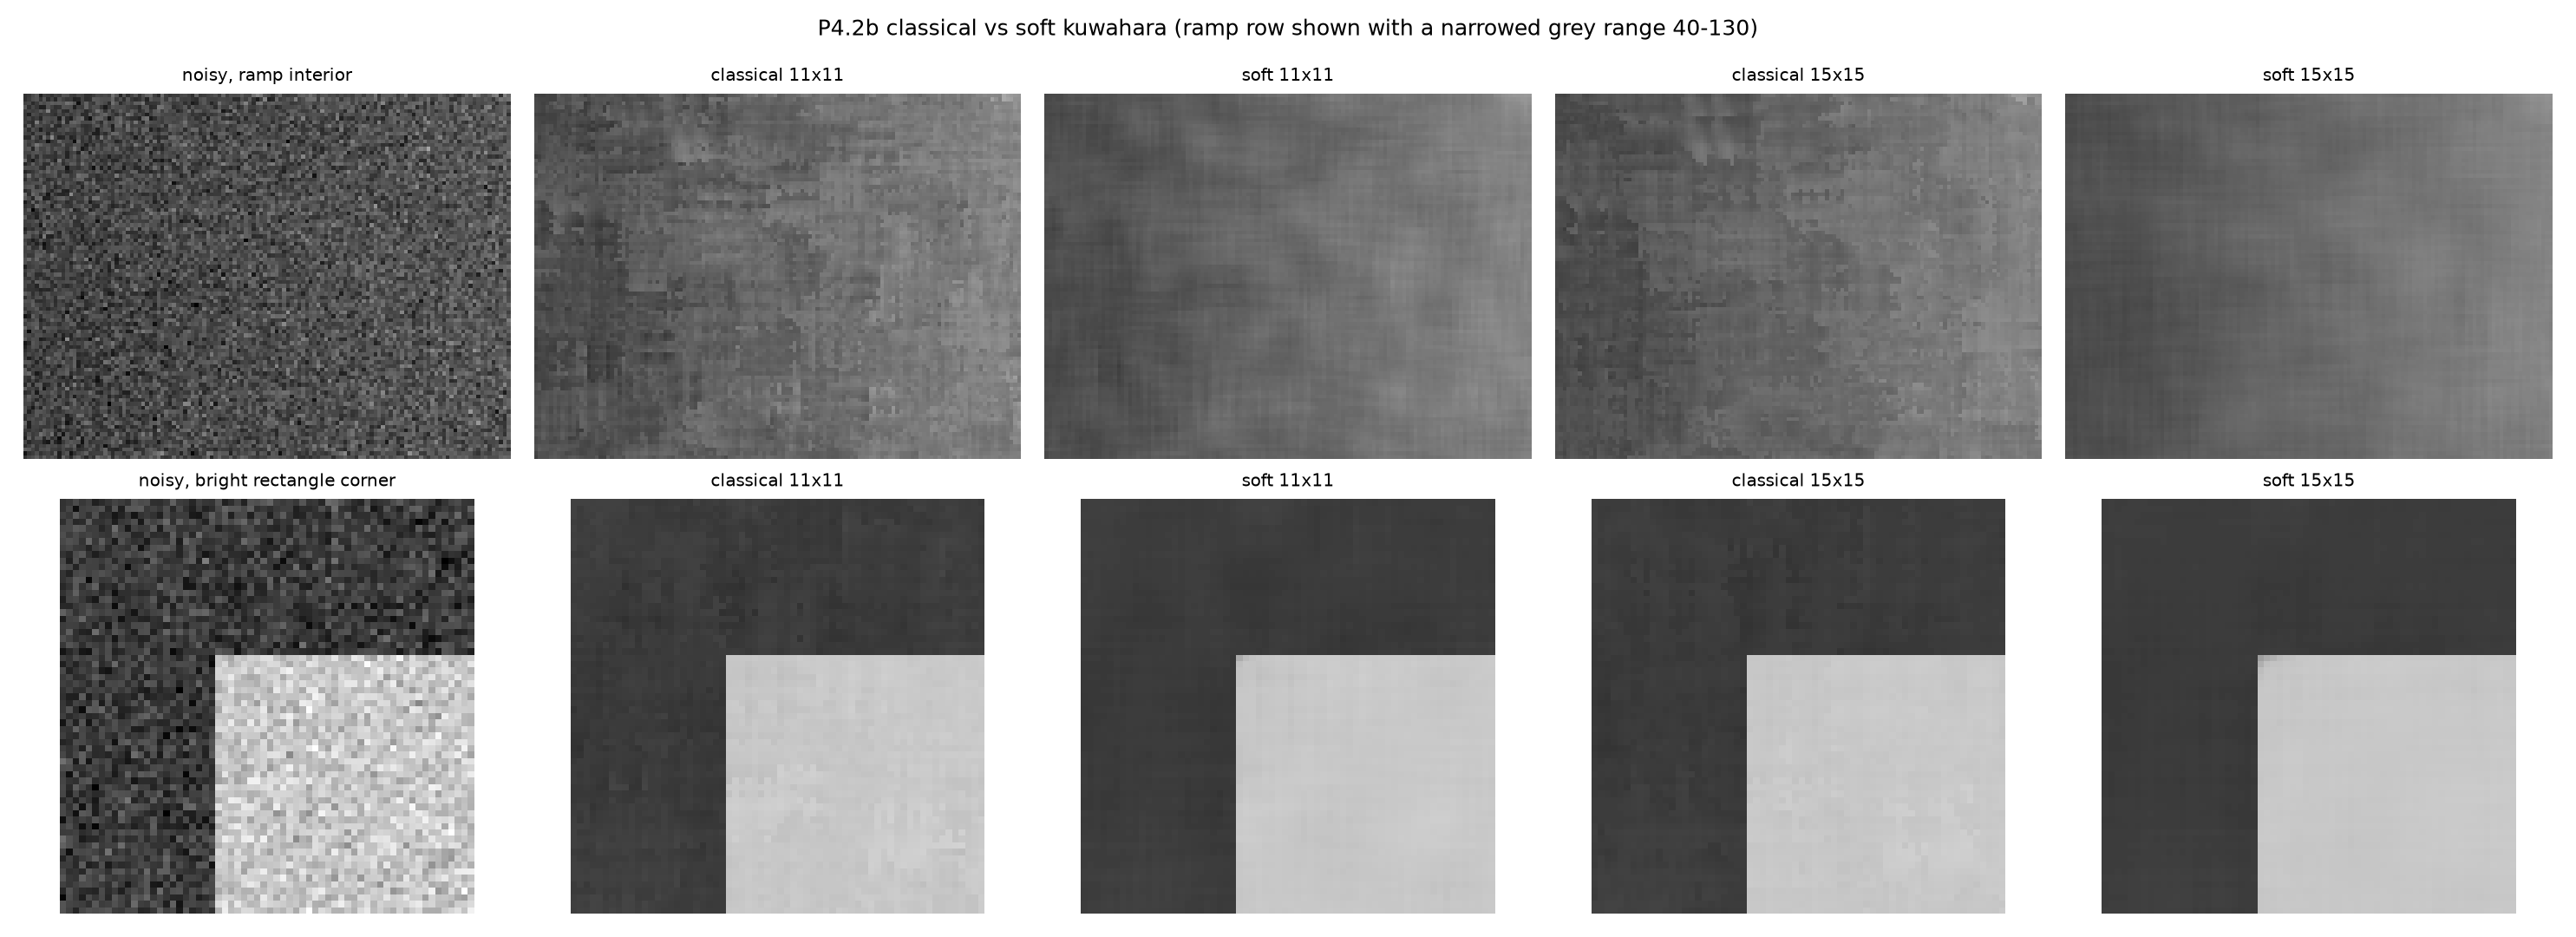
\includegraphics[width=\linewidth]{problem_4/blockiness.png}
\caption{Classical and soft Kuwahara at $11\times11$ and $15\times15$. Top: the
inside of the ramp, shown with a narrowed grey range of 40 to 130. Bottom: the
rectangle corner.}
\label{fig:block}
\end{figure}

\paragraph{(c) Operations per pixel.} I count additions and subtractions
(including comparisons), multiplications and divisions, and exponentials for one
output pixel.
\begin{itemize}
\item \emph{Kuwahara with integral images:} building the two integral images
costs 1 square and 4 additions. Each of the four sub-windows costs 6 additions or
subtractions for the two box sums, 1 subtraction for the variance and 3
multiplications or divisions. The argmin is 3 comparisons. Total: 35, 13, 0, the
same for every $N$.
\item \emph{Kuwahara with direct sums:} $4\cdot2((a+1)^2-1)+7$ additions and
$4(a+1)^2+12$ multiplications, i.e.\ $O(N^2)$.
\item \emph{Soft Kuwahara:} the integral-image count plus 4 subtractions, 4
divisions by $T$ and 4 exponentials for the weights, and 6 additions, 4
multiplications and 1 division for the weighted mean. Total: 45, 22, 4.
\item \emph{Bilateral:} per window tap, 1 subtraction, 1 square, 1 scaling, 1
exponential, 1 multiplication by the spatial weight, 1 by the value and 2
additions, plus one division per pixel: $3N^2$, $4N^2+1$, $N^2$.
\end{itemize}

\begin{table}[H]
\centering
\begin{tabular}{rlrrrr}
\toprule
$N$ & filter & add/sub/cmp & mult/div & exp & runtime (s)\\
\midrule
5 & Kuwahara (integral) & 35 & 13 & 0 & 0.0148\\
5 & soft Kuwahara & 45 & 22 & 4 & 0.0151\\
5 & bilateral & 75 & 101 & 25 & 0.0355\\
7 & Kuwahara (integral) & 35 & 13 & 0 & 0.0143\\
7 & Kuwahara (direct) & 127 & 76 & 0 & not timed\\
7 & bilateral & 147 & 197 & 49 & 0.0644\\
11 & Kuwahara (integral) & 35 & 13 & 0 & 0.0152\\
11 & bilateral & 363 & 485 & 121 & 0.1595\\
15 & Kuwahara (integral) & 35 & 13 & 0 & 0.0135\\
15 & soft Kuwahara & 45 & 22 & 4 & 0.0144\\
15 & bilateral & 675 & 901 & 225 & 0.3037\\
\bottomrule
\end{tabular}
\caption{Operation counts per pixel and measured run times on the $512\times512$
noisy image, median of 3 runs (all rows in \code{complexity.txt}). The
$15\times15$ bilateral uses $\sigma_s=3.5$, $\sigma_r=40$, since I did not
compute a matched pair at that size.}
\label{tab:complexity}
\end{table}

The bilateral filter is by far the most expensive per pixel. It needs an
exponential for every tap, because the range weight depends on the intensity
difference and cannot be computed in advance, and its work grows with the window
area ($N^2$ exponentials). Kuwahara only needs box statistics, which integral
images give in constant time, so its run time stays around 0.014 s from
$5\times5$ to $15\times15$ while the bilateral filter grows from 0.036 to
0.304 s. The four exponentials of the soft version add at most about 0.001 s.

\subsection{Breakdown of the bilateral filter}

\paragraph{(a, b) Experiment.} Each test image is $256\times128$, split into
$I_1=100$ and $I_2=150$ ($|\Delta I|=50$), with fresh Gaussian noise for every
NCR $=\sigma/|\Delta I|$ from 0.05 to 1.5 and 8 noise images per value (seed
$1000\cdot\text{index}+k$). The bilateral filter uses $\sigma_s=2$, radius 6,
and $\sigma_r=2\sigma$, a typical setting, since the range scale has to exceed
the noise for the filter to smooth at all. My edge-preservation metric is the
largest jump between neighbouring columns of the output profile, averaged over
rows and over the eight images, divided by $|\Delta I|$: 1 means the step is still
one pixel wide. A plain spatial Gaussian with the same $\sigma_s$ keeps 0.1997. I
define $\text{NCR}^*$ as the NCR where the curve falls to halfway between these
two levels, i.e.\ to 0.5998.

\begin{figure}[H]
\centering
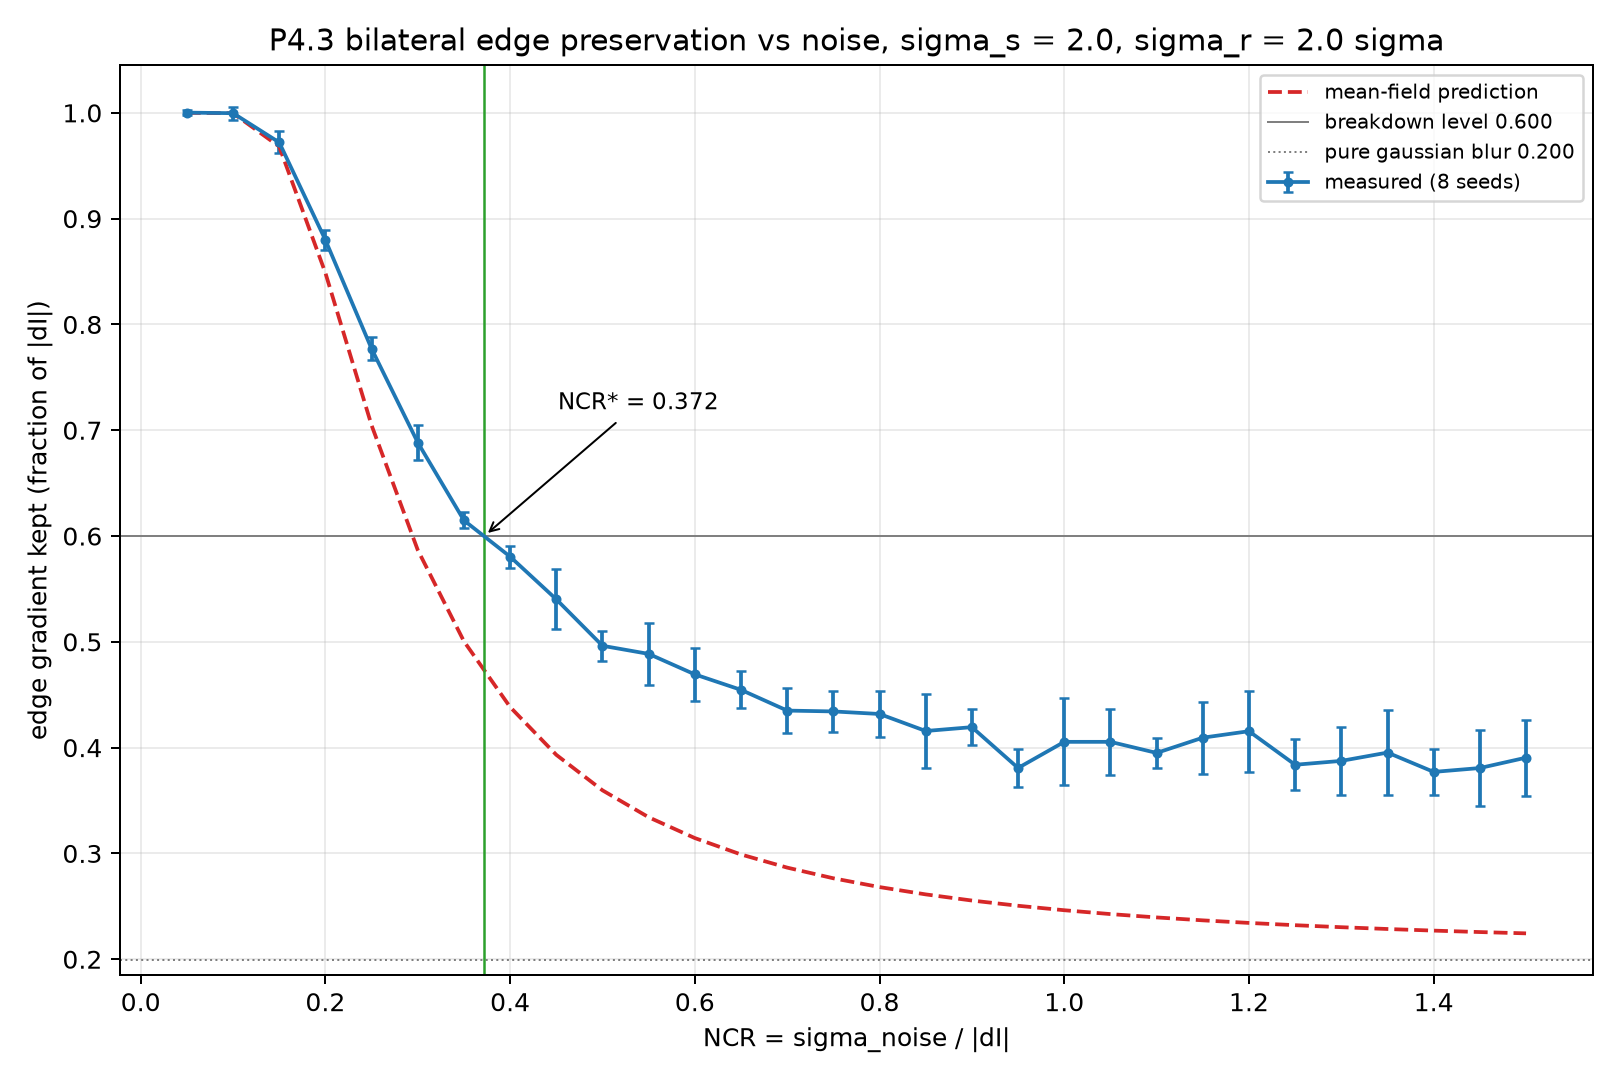
\includegraphics[width=0.75\linewidth]{problem_4/ncr_breakdown.png}
\caption{Fraction of the edge gradient kept against NCR (mean and spread over 8
noise images), with the mean-field prediction and the measured $\text{NCR}^*$.}
\label{fig:ncr}
\end{figure}

\begin{table}[H]
\centering
\begin{tabular}{rrrrrr}
\toprule
NCR & gradient kept & spread & edge RMSE & mean-field & $\rho$\\
\midrule
0.10 & 0.9997 & 0.0061 & 1.484 & 0.9997 & 0.0002\\
0.20 & 0.8799 & 0.0093 & 4.815 & 0.8487 & 0.1245\\
0.30 & 0.6884 & 0.0166 & 8.375 & 0.5868 & 0.3962\\
0.35 & 0.6148 & 0.0077 & 9.719 & 0.5005 & 0.5065\\
0.40 & 0.5805 & 0.0105 & 10.583 & 0.4384 & 0.5940\\
0.50 & 0.4963 & 0.0141 & 12.340 & 0.3596 & 0.7165\\
1.00 & 0.4055 & 0.0412 & 18.102 & 0.2463 & 0.9200\\
1.50 & 0.3905 & 0.0358 & 23.621 & 0.2244 & 0.9636\\
\bottomrule
\end{tabular}
\caption{Selected rows of \code{ncr\_breakdown.txt}. Edge RMSE in grey levels.}
\label{tab:ncr}
\end{table}

The measured curve crosses that level at $\textbf{NCR}^*\mathbf{=0.372}$. Below
about 0.15 the step survives intact, and by 0.5 half of its gradient is gone
(examples in \code{ncr\_examples.png}).

\paragraph{(c) Why it breaks down.} The range kernel
$w_r(\Delta I)=e^{-\Delta I^2/2\sigma_r^2}$ is supposed to give small weight to
neighbours across the edge and large weight to neighbours on the same side. With
noise, the difference the filter actually sees is $d=f(\mathbf p)-f(\mathbf q)$,
which is distributed as $\mathcal N(0,2\sigma^2)$ on the same side and
$\mathcal N(\Delta I,2\sigma^2)$ across the edge. Averaging the Gaussian kernel
over a Gaussian difference gives
\begin{equation}
\operatorname{E}[w_r]=\frac{\sigma_r}{\sqrt{\sigma_r^2+2\sigma^2}}\cdot
\begin{cases}1&\text{same side}\\ e^{-\Delta I^2/2(\sigma_r^2+2\sigma^2)}&\text{across}\end{cases},
\qquad
\rho=\exp\!\Big(-\frac{\Delta I^2}{2(\sigma_r^2+2\sigma^2)}\Big)=\exp\!\Big(-\frac{1}{2\,\text{NCR}^2(k^2+2)}\Big),
\end{equation}
with $\sigma_r=k\sigma$ and $\rho$ the ratio of the expected cross-edge weight to
the same-side weight. The noise widens the effective range kernel from $\sigma_r$
to $\sqrt{\sigma_r^2+2\sigma^2}$. Once that width is comparable to the step,
$\rho$ approaches 1 and neighbours across the edge are trusted almost as much as
those on the same side, so the filter turns into a spatial blur. $\rho$ passes
$1/2$ at $\text{NCR}=1/\sqrt{2\ln2\,(k^2+2)}=0.347$ for $k=2$, close to the
measured 0.372. The change is gradual because $\rho$ rises smoothly, from 0.12 at
NCR 0.2 to 0.72 at 0.5.

Plugging the expected weights in place of the random ones (the ``mean-field''
column, which also gives the centre pixel its exact weight of 1) predicts the
onset fairly well, crossing the midpoint at 0.2945. It does not predict the
high-noise level: the measured curve levels off at 0.395 instead of falling
towards 0.2. The model treats the weights as independent of the values, but they
are not: neighbours whose noisy values happen to be close to the centre pixel's
value get the largest weights, which pulls the output towards the centre pixel
and keeps part of the step. Because $\sigma_r$ grows with $\sigma$, this does not
fade as the noise grows. Measured against that plateau instead of the Gaussian
level, the halfway point is at NCR 0.295.

\section{Denoising and the Wiener filter}

\textbf{Data.} The instructor's clean RGB reference (\code{reference\_image.jpg},
$2048\times3072$) is box-averaged $2\times2$ to $1024\times1536$ and scaled to
$[0,1]$. The result is still at least $1024\times1024$, and the averaging removes
some of the JPEG noise of the ``clean'' reference. The same image is used in
Problem 6. Noise is added as $g=f+(\sigma/255)z$ with a single standard-normal field
$z$ (seed 2026) shared by every method and every $\sigma$, and $g$ is never clipped
before filtering.

\subsection{The Wiener filter as an MMSE denoiser}

\paragraph{Derivation.} Let $f$ and $n$ be zero-mean (after removing the mean),
uncorrelated, wide-sense stationary fields with power spectra $S_{ff}$ and $S_{nn}$,
and $g=f+n$. For stationary fields the DFT coefficients at different frequencies are
(asymptotically) uncorrelated, so the best linear estimate in the frequency domain
can be found one frequency at a time: look for $\hat F=WG$ minimising
$\operatorname{E}|F-WG|^2$. The minimum satisfies the orthogonality condition, which
says that the error is uncorrelated with the data:
\begin{equation}
\operatorname{E}\big[(F-WG)\,\overline{G}\big]=0
\;\Longrightarrow\;
\operatorname{E}[F\overline{G}]=W\,\operatorname{E}|G|^2 .
\end{equation}
Because $f$ and $n$ are uncorrelated, $\operatorname{E}[F\overline G]=\operatorname{E}|F|^2=S_{ff}$
and $\operatorname{E}|G|^2=S_{ff}+S_{nn}$, so
\begin{equation}
\hat F(u,v)=W(u,v)G(u,v),\qquad W=\frac{S_{ff}}{S_{ff}+S_{nn}},
\end{equation}
with remaining error $S_{ff}S_{nn}/(S_{ff}+S_{nn})$ at each frequency.

\paragraph{Estimating the spectra.} $S_{nn}$ comes from the known injected variance.
For white noise of per-pixel variance $\sigma^2$ on the unnormalised $P\times P$ DFT,
Parseval gives $\operatorname{E}|N(u,v)|^2=P^2\sigma^2$ at every frequency. $S_{ff}$
is estimated from the data alone:
\begin{equation}
\hat S_{ff}=\max\big(\overline{|G|^2}-P^2\sigma^2,\;0\big),
\end{equation}
where $\overline{|G|^2}$ is the noisy periodogram averaged over rings of unit width
around the origin (``radial''). This assumes the image spectrum is isotropic, the
noise white, stationary and independent of the signal, and that averaging over a
ring removes enough of the periodogram's variance; the floor at zero handles rings
where the noise estimate exceeds the measured power. A second version replaces the
ring average with a $15\times15$ box average in the frequency plane (``smoothed''),
which keeps anisotropy. Every frequency-domain filter in this problem mirror-pads to
$P=3072$ so that no low-pass darkens the borders; $W$ is applied per colour channel.

\paragraph{Comparison.} The Gaussian and Butterworth ($n=2$) low-pass filters are
\code{make\_filter} from Problem 2, with $D_0$ tuned by PSNR against the clean
reference on a 20-point log grid plus a 9-point refinement. The bilateral filter is
the Problem 4 implementation extended to colour (the range distance is the Euclidean
distance between RGB vectors), with $\sigma_s\in\{0.5,1,1.5,2,3\}$ and
$\sigma_r=k\sigma$, $k\in\{1,1.5,2,3,4,6\}$, tuned on a central $512\times512$ crop.
Every chosen value lies inside its grid. These three use the clean image, so they
are labelled oracle-tuned. So is the ``oracle'' Wiener filter, which uses the clean
periodogram as $S_{ff}$ and shows what perfect spectrum knowledge would give.

\begin{table}[H]
\centering
\small
\begin{tabular}{rlrr}
\toprule
$\sigma$ & method (parameters) & PSNR (dB) & SSIM\\
\midrule
5 & noisy input & 34.288 & 0.8703\\
 & Wiener, radial $\hat S_{ff}$ & 36.211 & 0.9219\\
 & Wiener, smoothed $\hat S_{ff}$ & 36.309 & 0.9231\\
 & Wiener, clean periodogram (oracle) & 37.237 & 0.9334\\
 & Gaussian LPF $D_0=1327$ (oracle-tuned) & 36.096 & 0.9196\\
 & Butterworth $n=2$ $D_0=1400$ (oracle-tuned) & 36.185 & 0.9213\\
 & bilateral $\sigma_s=1$, $\sigma_r=3\sigma$ (oracle-tuned) & \textbf{38.025} & \textbf{0.9520}\\
\midrule
10 & noisy input & 28.405 & 0.6715\\
 & Wiener, radial $\hat S_{ff}$ & 32.250 & 0.8434\\
 & Wiener, smoothed $\hat S_{ff}$ & 32.345 & 0.8428\\
 & Wiener, clean periodogram (oracle) & 33.350 & 0.8642\\
 & Gaussian LPF $D_0=862$ (oracle-tuned) & 32.234 & 0.8395\\
 & Butterworth $n=2$ $D_0=960$ (oracle-tuned) & 32.192 & 0.8419\\
 & bilateral $\sigma_s=1$, $\sigma_r=3\sigma$ (oracle-tuned) & \textbf{33.872} & \textbf{0.8801}\\
\midrule
20 & noisy input & 22.658 & 0.4030\\
 & Wiener, radial $\hat S_{ff}$ & 29.137 & 0.7373\\
 & Wiener, smoothed $\hat S_{ff}$ & 29.166 & 0.7291\\
 & Wiener, clean periodogram (oracle) & 30.185 & 0.7694\\
 & Gaussian LPF $D_0=531$ (oracle-tuned) & 29.132 & 0.7366\\
 & Butterworth $n=2$ $D_0=624$ (oracle-tuned) & 29.007 & 0.7323\\
 & bilateral $\sigma_s=1.5$, $\sigma_r=3\sigma$ (oracle-tuned) & \textbf{30.269} & \textbf{0.7698}\\
\midrule
40 & noisy input & 17.175 & 0.1856\\
 & Wiener, radial $\hat S_{ff}$ & 26.751 & 0.6216\\
 & Wiener, smoothed $\hat S_{ff}$ & 26.638 & 0.5925\\
 & Wiener, clean periodogram (oracle) & \textbf{27.697} & \textbf{0.6622}\\
 & Gaussian LPF $D_0=310$ (oracle-tuned) & 26.697 & 0.6214\\
 & Butterworth $n=2$ $D_0=345$ (oracle-tuned) & 26.595 & 0.6227\\
 & bilateral $\sigma_s=2$, $\sigma_r=4\sigma$ (oracle-tuned) & 27.185 & 0.6328\\
\bottomrule
\end{tabular}
\caption{Denoising the reference image (\code{denoising\_table.txt}). $\sigma$ is in
8-bit levels; images are in $[0,1]$; outputs are clipped to $[0,1]$ for the metrics,
data range 1.0; SSIM \cite{wang} is \code{skimage.metrics.structural\_similarity} ($7\times7$
uniform window, $K_1=0.01$, $K_2=0.03$, averaged over the three channels). LPF radii
are in bins of the $3072\times3072$ grid. Bold: best in each block.}
\label{tab:denoise}
\end{table}

\begin{figure}[H]
\centering
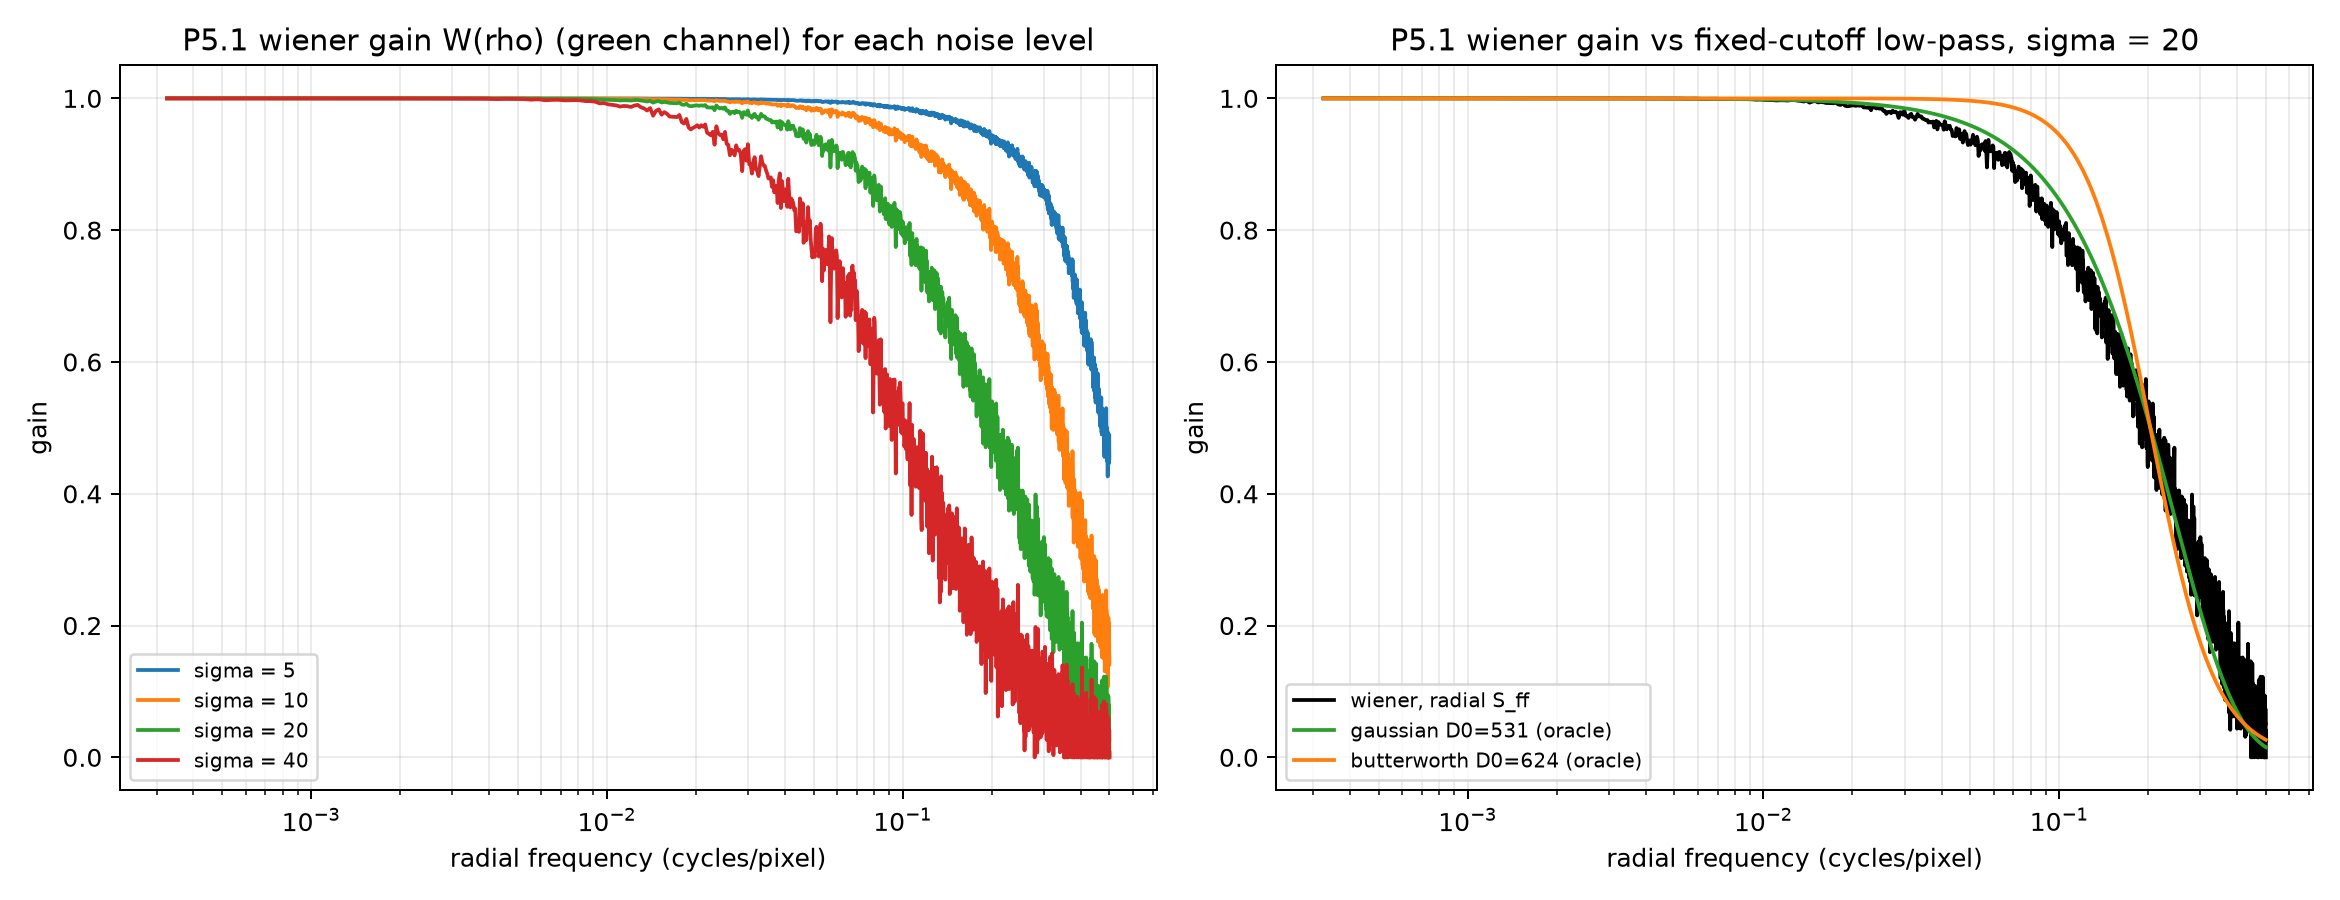
\includegraphics[width=0.95\linewidth]{problem_5/wiener_gain.png}
\caption{Left: the estimated Wiener gain (green channel) against radial frequency
for each $\sigma$. Right: at $\sigma=20$, the Wiener gain against the oracle-tuned
low-pass filters.}
\label{fig:gain}
\end{figure}

\paragraph{How the shrinkage behaves.} $W=1/(1+S_{nn}/S_{ff})$ depends only on the
local signal-to-noise ratio at each frequency. Natural-image power falls steeply
with frequency while white noise is flat, so $W$ stays near 1 at low frequencies,
where the image dominates, and falls towards 0 where the image power drops below
the noise. When $\sigma$ grows, $S_{nn}$ rises at every frequency and the crossover
moves down (Fig.~\ref{fig:gain}, left; \code{wiener\_gain.txt}): the gain at 0.1
cycles/pixel is 0.985 at $\sigma=5$ and 0.510 at $\sigma=40$, and the frequency where
it falls to one half drops from 0.470 to 0.088 cycles/pixel. A fixed-cutoff low-pass filter has the
same general shape, but its cutoff and roll-off are fixed in advance and have to be
tuned to each noise level and image. The Wiener gain sets its own shape from the
measured spectrum, uses no reference, and its roll-off follows the image rather
than a formula. At $\sigma=20$ the oracle-tuned Gaussian ended up with almost the
same curve as the estimated Wiener gain (Fig.~\ref{fig:gain}, right), which is why
the two score 29.132 and 29.137 dB. Across all four noise levels the untuned radial
Wiener filter matches or beats the oracle-tuned low-pass filters, and the oracle
Wiener filter is about 1 dB higher still, which is the cost of estimating $S_{ff}$
from noisy data. The 2-D smoothed estimate is slightly better than the radial one
at low noise and worse at $\sigma=40$ (SSIM 0.5925 against 0.6216). A
$15\times15$ box averages far fewer periodogram values than a full ring, and where
$S_{ff}$ is close to $S_{nn}$ the subtraction amplifies that extra variance into
patches of frequencies where noise is let through.

Wiener does not win every comparison. The oracle-tuned bilateral filter beats the
radial Wiener filter at every $\sigma$ (by 1.8 dB at $\sigma=5$ and 0.4 dB at
$\sigma=40$), and beats even the oracle Wiener filter for $\sigma\le20$. Wiener's
optimality is among \emph{linear} estimators, under second-order statistics of a
stationary model; the bilateral filter is nonlinear and adapts its averaging at
every pixel. In fairness, the bilateral result had two parameters tuned against the
clean image, while the radial Wiener filter used only $\sigma$.

\begin{figure}[H]
\centering
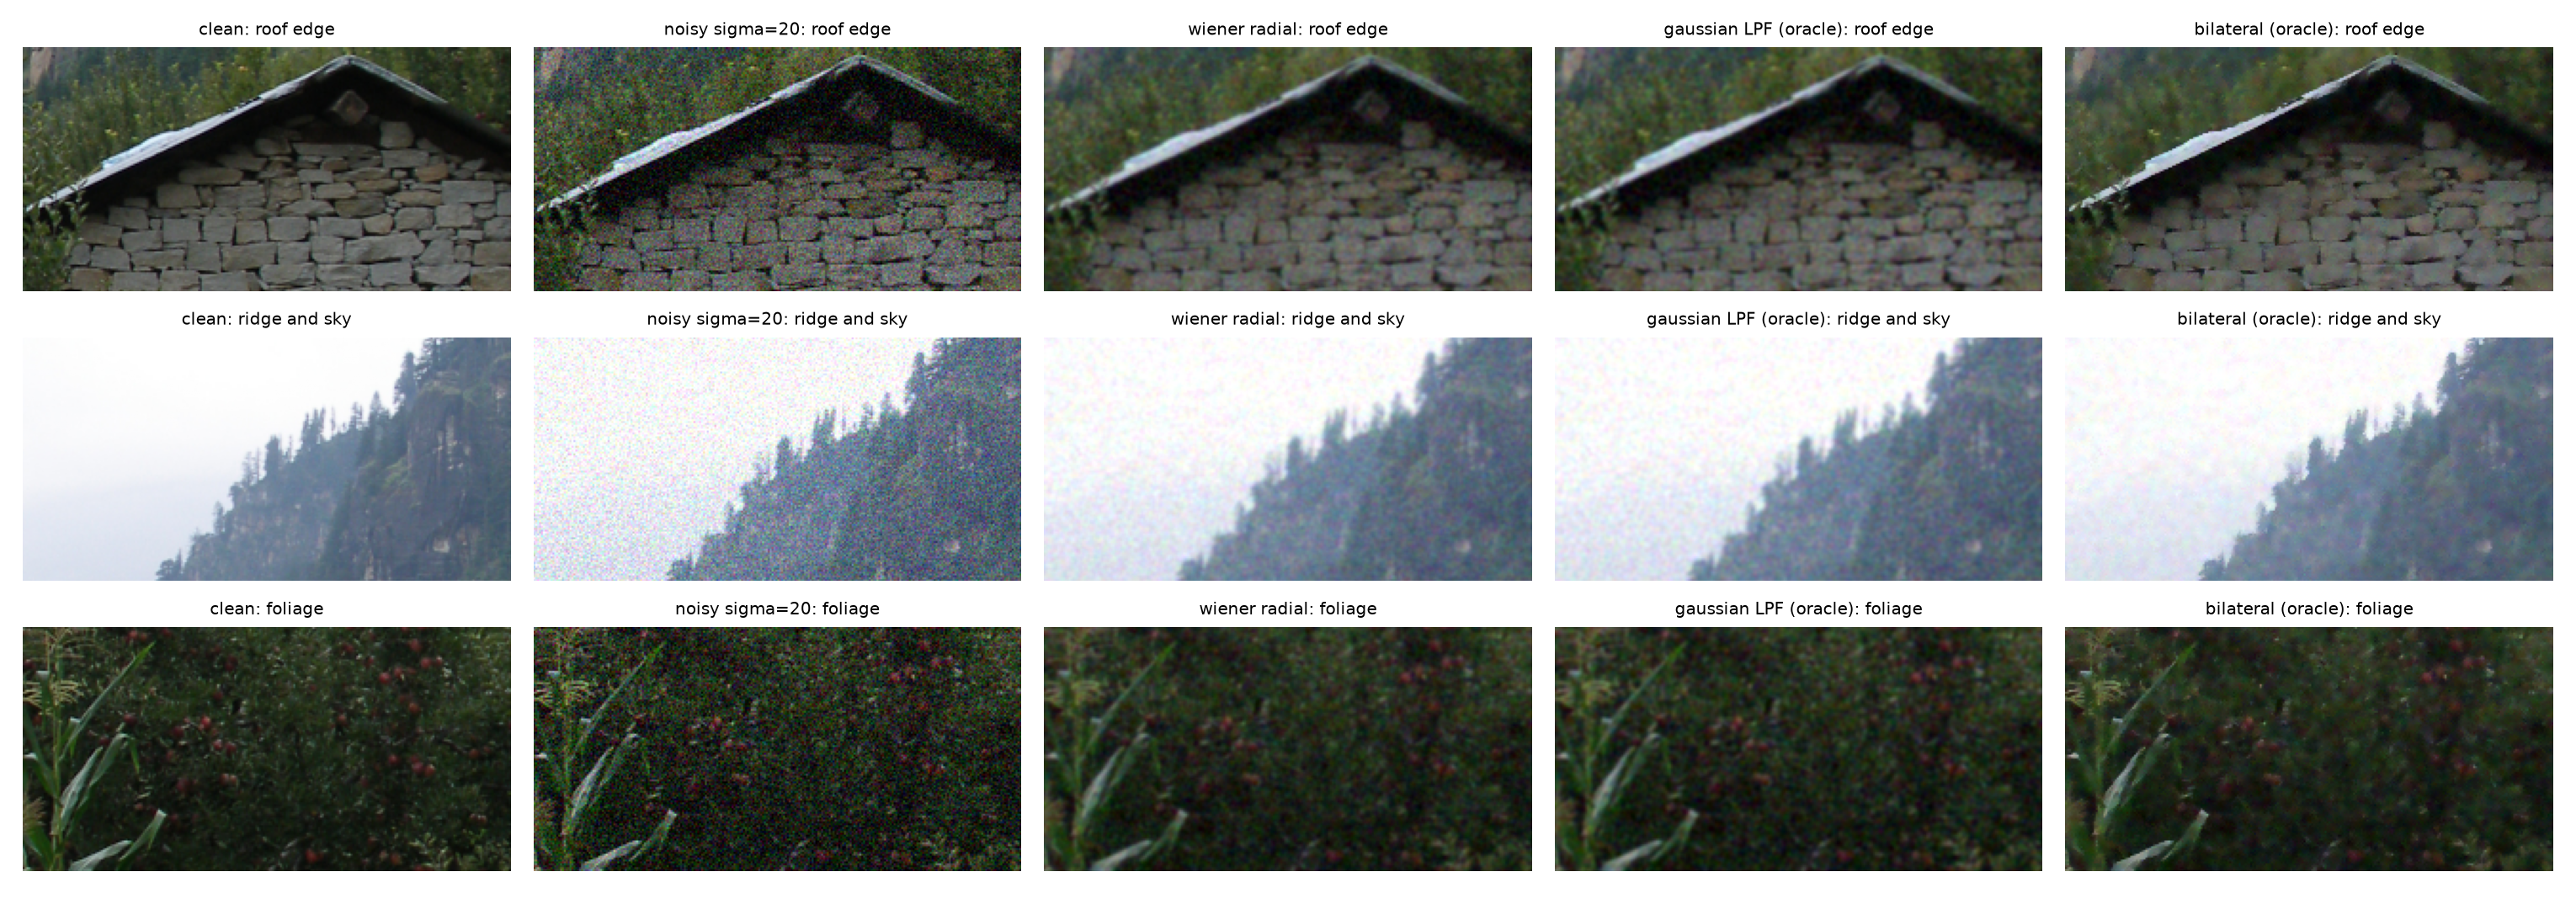
\includegraphics[width=\linewidth]{problem_5/denoising_crops.png}
\caption{Crops at $\sigma=20$: roof edge, ridge against sky, foliage.}
\label{fig:denoise-crops}
\end{figure}

\subsection{Testing the assumptions}

\paragraph{Mis-specified noise power.} At $\sigma=20$ the radial Wiener filter was run
assuming noise power $0.5S_{nn}$, $S_{nn}$ and $2S_{nn}$, with $\hat S_{ff}$
re-estimated each time as a user of the filter would. The error is split into a
flat band (the 50\,\% of pixels with the smallest clean-image gradient) and an edge
band (the largest 10\,\%), in 8-bit levels.

\begin{table}[H]
\centering
\begin{tabular}{rrrrrr}
\toprule
assumed & PSNR (dB) & SSIM & flat RMSE & edge RMSE & mean gain\\
\midrule
$0.5S_{nn}$ & 26.389 & 0.5633 & 11.533 & 13.959 & 0.5980\\
$S_{nn}$ & 29.137 & 0.7373 & 6.910 & 14.987 & 0.1992\\
$2S_{nn}$ & 27.644 & 0.7038 & 6.767 & 20.257 & 0.0473\\
\bottomrule
\end{tabular}
\caption{Noise-power mis-specification at $\sigma=20$ (\code{misspecification.txt}).}
\label{tab:misspec}
\end{table}

With the subtraction estimate, the gain is $W=1-\alpha S_{nn}/\overline{|G|^2}$
(floored at 0) for an assumed power $\alpha S_{nn}$. At high frequencies, where
$\overline{|G|^2}\approx S_{nn}$ (pure noise), the correct filter gives
$W\approx0$, but $\alpha=0.5$ gives $W\approx0.5$, so half of the noise amplitude
there passes through. The mean gain triples, the flat-region error rises from 6.9 to
11.5 levels, and residual noise is visible everywhere (\code{misspecification.png}).
With $\alpha=2$ every frequency whose power is below twice the noise is removed,
including the frequencies that carry fine edges. The flat error barely changes
(6.77), but the edge error rises from 15.0 to 20.3 and the image looks smoothed. The
two failures are not symmetric: underestimation leaves noise where the image is
flat, overestimation blurs where it is not.

\paragraph{Why a correct Wiener filter still blurs edges.}

\begin{table}[H]
\centering
\begin{tabular}{lrrr}
\toprule
Method ($\sigma=20$) & flat RMSE & edge RMSE & edge / flat\\
\midrule
noisy input & 18.016 & 19.697 & 1.09\\
Wiener, radial & 6.910 & 14.987 & 2.17\\
Wiener, oracle & 6.382 & 12.401 & 1.94\\
Gaussian LPF (oracle-tuned) & 6.961 & 14.911 & 2.14\\
bilateral (oracle-tuned) & 5.935 & 12.009 & 2.02\\
\bottomrule
\end{tabular}
\caption{Where the remaining error sits (\code{edge\_blur.txt}).}
\label{tab:edge-blur}
\end{table}

Even with the correct noise power, the Wiener filter's error at edges is more than
twice its error in flat regions (Table~\ref{tab:edge-blur}), and the roof-edge profile
(\code{edge\_profile.png}) shows the bright roof line flattened from a luminance of
0.758 to 0.495 (0.567 even with the oracle spectrum), while the bilateral filter
keeps it at 0.770. The filter is linear and shift-invariant, so one gain $W(u,v)$ applies at every
pixel. $S_{ff}$ is an average over the whole image, which is mostly smooth
foliage, sky and mountain, so at high frequencies it is small and $W$ cuts them.
An edge is a local event whose energy is spread over all frequencies, including
those high ones, so it loses them too, even though near the edge the local signal
power at high frequency is far above the noise. MMSE optimality only promises the
smallest mean squared error averaged over the image and over the noise, among linear
filters, for a stationary model described by its second-order statistics. It does
not promise small error at any particular place, and edges are a small fraction of
the pixels, so the average can be minimised while they are blurred. A natural
image is not a stationary Gaussian field: its edges are sparse and localised. A
nonlinear filter that looks at local intensities, such as the bilateral filter,
achieves both lower flat and lower edge error here (5.9 and 12.0).

\paragraph{Real noisy photograph: blocked.} This part needs a genuinely noisy
photograph taken by the student, and none had been supplied when this report was
produced (\code{real\_noise.txt} records the blocked run). The case study is
implemented and runs automatically once a file named \code{noisy*} is placed in
\code{photos/}. It estimates $\sigma$ per channel with Immerkær's method \cite{immerkaer}, applies the
white-noise radial Wiener filter at full resolution, and compares crops, residuals,
residual spectra, residual autocorrelation and residual level against brightness
with a synthetic white-noise case at the same $\sigma$, without PSNR or SSIM. The
noise estimator was validated on the synthetic images: injected $\sigma$ of 5, 10, 20
and 40 are estimated as 5.895, 10.531, 20.278 and 40.125, and the clean reference
itself gives 2.540, the floor set by fine image texture and the reference's own
noise. Real camera noise is expected to depart from the white-noise model in four
ways the analysis is built to show: shot noise makes its variance depend on
brightness, demosaicing correlates neighbouring pixels and colours, in-camera
sharpening boosts its high frequencies, and JPEG compression removes some of them
in $8\times8$ blocks.

\paragraph{Conclusion.} The Wiener gain adapts its cut-off to the measured spectrum
and the noise level, and without any tuning it matches low-pass filters tuned on the
clean image. Its optimality is limited to linear filters under a stationary model:
it blurs edges even when the noise power is right, it degrades in opposite ways
when the noise power is wrong, and a tuned nonlinear filter beat it here.

\section{Motion blur and deblurring}

For the synthetic experiments the clean image is the $1024\times1536$ RGB
reference from Problem 5, in $[0,1]$. I put $x$ to the right and $y$ up, and
measure the motion angle $\theta$ counter-clockwise from the $+x$ axis. In array
terms, a point $t$ along the motion sits at column $+t\cos\theta$ and row
$-t\sin\theta$ from the centre. Frequencies $f_x,f_y$ are in cycles per pixel
with the same orientation.

\subsection{Model and synthesis}

\paragraph{PSF.} During the exposure the scene moves uniformly by a total
distance $L$ along $(\cos\theta,\sin\theta)$. Each scene point is therefore
recorded with equal weight along a segment of length $L$ centred on its true
position:
\begin{equation}
h(x,y)=\frac1L\int_{-L/2}^{L/2}\delta(x-t\cos\theta,\;y-t\sin\theta)\,dt .
\end{equation}
Integrating over the plane gives $\frac1L\int_{-L/2}^{L/2}1\,dt=1$, so the blur
keeps the mean brightness. To discretise it, \code{motion\_psf} integrates $h$
over each pixel: a pixel's weight is the length of the segment inside its unit
square divided by $L$. I compute this by sampling the segment at 50 midpoints per
pixel and counting how many samples land in each pixel, then normalise the
weights to sum to exactly one. For $L=21$, $\theta=30^\circ$ the kernel is
$25\times25$ with 29 non-zero taps (\code{psf\_otf.png}). A horizontal segment
with integer $L$ becomes exactly $L$ taps of $1/L$, which the unit tests check.

\paragraph{Boundary convention.} I use circular convolution for the forward blur
and for every deconvolution: $g=\mathcal F^{-1}\{H\cdot\mathcal F\{f\}\}+n$, with
$H$ the DFT of the PSF placed with its centre at index $(0,0)$ of the image grid.
The forward model and the inverse filters are then exactly consistent, and no
pixels have to be cropped before measuring.

\paragraph{Noise.} White Gaussian noise is added to the blurred image at
\begin{equation}
\text{SNR}_\text{dB}=10\log_{10}\frac{\sum_{x,y,c}f(x,y,c)^2}{\sum_{x,y,c}n(x,y,c)^2}
\end{equation}
with $f$ the clean image, at 50, 40, 30 and 20 dB. The noise is one
standard-normal field (seed 2026) scaled to each level. The realised values are
50.000, 40.000, 30.000 and 20.000 dB (noise standard deviations 0.00159,
0.00503, 0.01589 and 0.05025), and the noisy image is not clipped.

\paragraph{OTF.} With
$\mathcal F\{h\}(f_x,f_y)=\iint h(x,y)\,e^{-j2\pi(f_xx+f_yy)}\,dx\,dy$, the delta
function collapses the double integral onto the segment. Writing
$p=f_x\cos\theta+f_y\sin\theta$,
\begin{equation}
H(f_x,f_y)=\frac1L\int_{-L/2}^{L/2}e^{-j2\pi tp}\,dt
=\frac1L\cdot\frac{e^{-j\pi Lp}-e^{j\pi Lp}}{-j2\pi p}
=\frac{\sin(\pi Lp)}{\pi Lp}=\sinc\big(L(f_x\cos\theta+f_y\sin\theta)\big).
\end{equation}
$H$ is real because the PSF is symmetric about its centre. It is zero where
$\sin(\pi Lp)=0$ with $p\ne0$, i.e.\ on the lines
\begin{equation}
f_x\cos\theta+f_y\sin\theta=\frac mL,\qquad m\in\mathbb Z\setminus\{0\}.
\end{equation}
$p$ is the component of the frequency vector $\mathbf f=(f_x,f_y)$ along the
motion direction $\mathbf u=(\cos\theta,\sin\theta)$. So neighbouring zeros are
$1/L$ apart along $\mathbf u$, and each zero set
$\{\mathbf f:\mathbf f\cdot\mathbf u=m/L\}$ is a straight line perpendicular to
$\mathbf u$: the zero lines are perpendicular to the motion direction in the
frequency plane. In words, blurring along $\mathbf u$ removes frequencies that
oscillate along $\mathbf u$, and $H$ does not change at all as you move
perpendicular to $\mathbf u$. For $L=21$ the spacing is $1/L=0.04762$
cycles/pixel.

The DFT samples $f_x=k/1536$ and $f_y=l/1024$, and the zero lines usually pass
between samples, so the sampled $|H|$ is small near them but not zero
(Table~\ref{tab:zeros}). The smallest sampled value on the grid is
$5.6\times10^{-9}$. Fig.~\ref{fig:otf} marks the sampled points closest to each
predicted line and compares $|H|$ along the motion axis with $|\sinc(Lp)|$. They
agree closely at low frequency (largest difference 0.0168 below 0.1
cycles/pixel) but differ by up to 0.51 overall. The largest difference is near a
corner of the frequency plane, at $p\approx0.5$. The PSF is sampled on the pixel
grid, so its spectrum is periodic, and $|H|$ rises again towards $p=\pm0.5$
(aliasing) while the continuous sinc keeps falling; the bumps near $p=\pm0.5$ in
the right panel of Fig.~\ref{fig:otf} show this.

\begin{table}[H]
\centering
\begin{tabular}{rrrrrr}
\toprule
$m$ & $m/L$ & samples near the line & min $|H|$ & median $|H|$ & $|\sinc|$ at $(m+\tfrac12)/L$\\
\midrule
1 & 0.04762 & 1183 & $1.33\times10^{-7}$ & $3.96\times10^{-3}$ & 0.2122\\
2 & 0.09524 & 1184 & $6.05\times10^{-6}$ & $4.54\times10^{-3}$ & 0.1273\\
3 & 0.14286 & 1182 & $5.74\times10^{-6}$ & $3.94\times10^{-3}$ & 0.0909\\
4 & 0.19048 & 1163 & $1.48\times10^{-5}$ & $1.18\times10^{-2}$ & 0.0707\\
5 & 0.23810 & 1051 & $2.64\times10^{-6}$ & $1.06\times10^{-2}$ & 0.0579\\
\bottomrule
\end{tabular}
\caption{The sampled OTF within half a frequency bin of each predicted zero line,
against the sidelobe peak between lines (\code{otf\_zeros.txt}). $m/L$ in
cycles/pixel.}
\label{tab:zeros}
\end{table}

\begin{figure}[H]
\centering
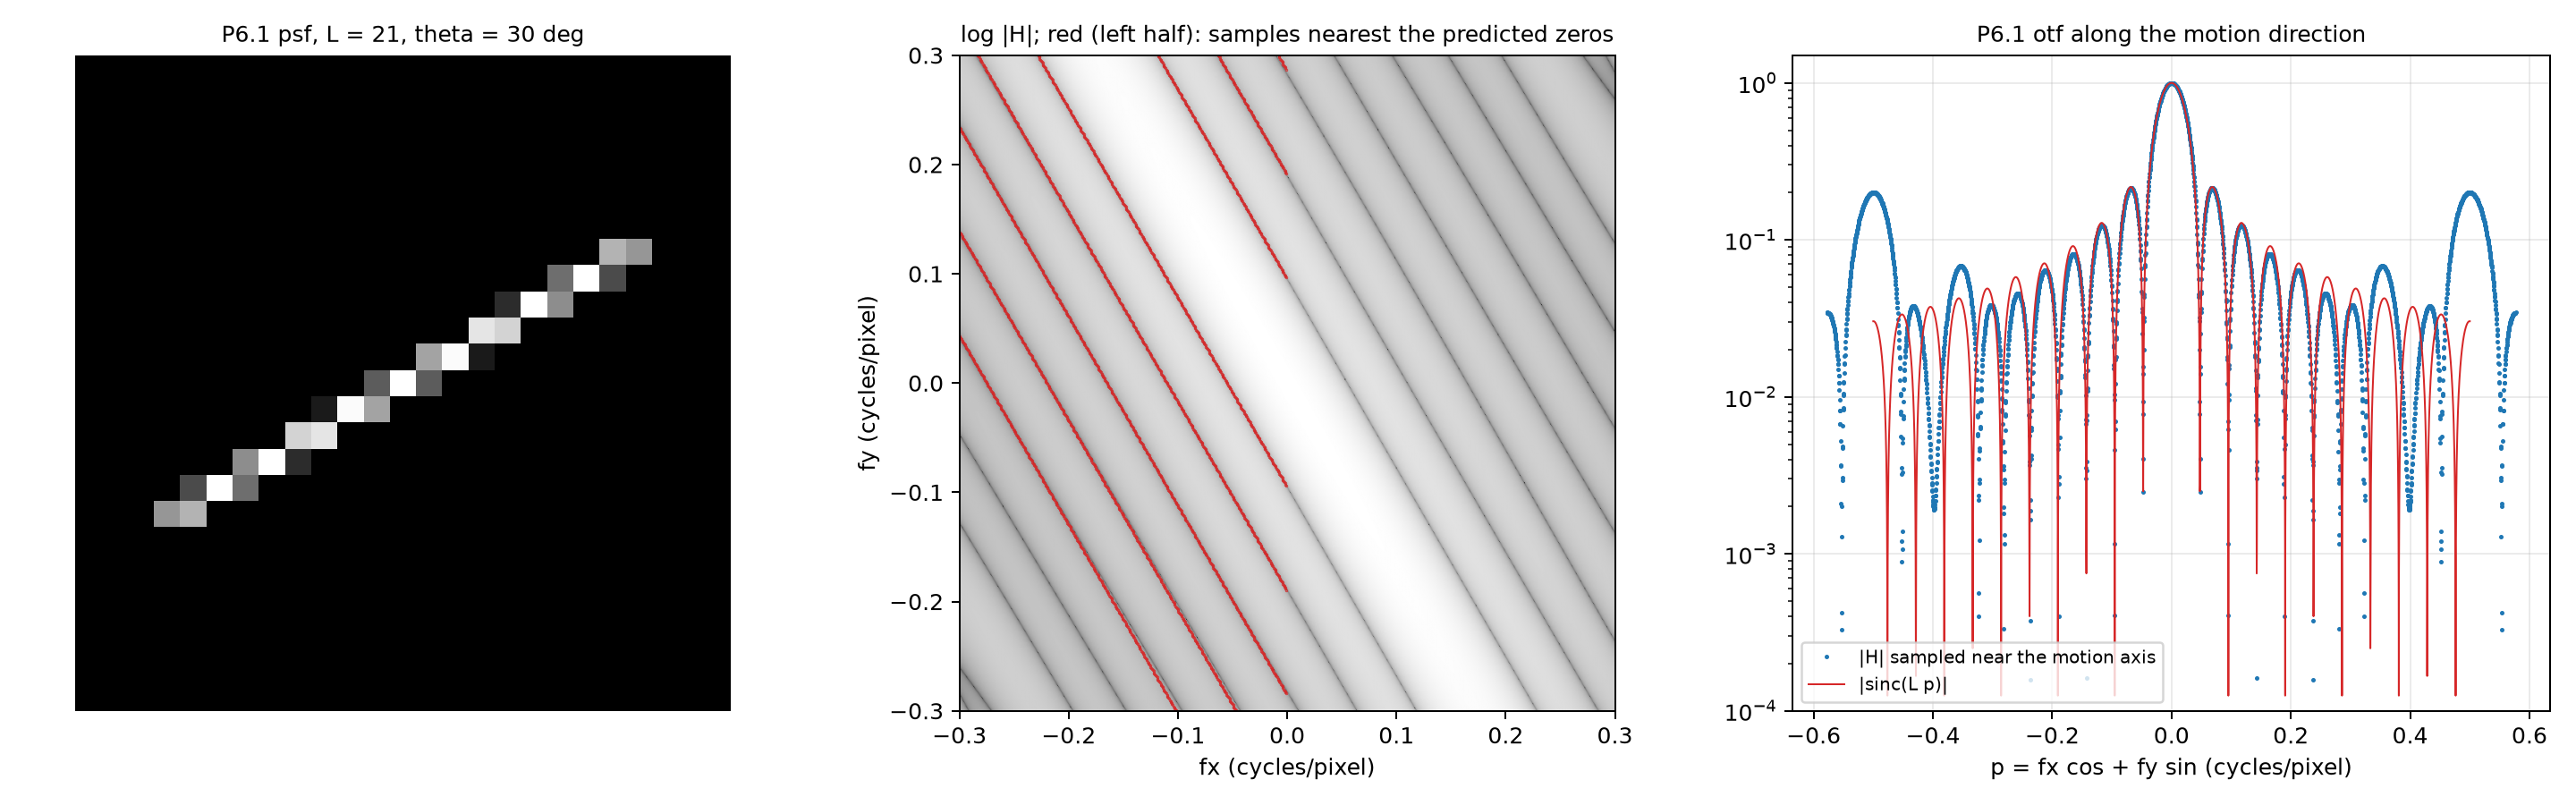
\includegraphics[width=\linewidth]{problem_6/psf_otf.png}
\caption{PSF ($L=21$, $\theta=30^\circ$); $\log|H|$ against $f_x,f_y$
(cycles/pixel) with the sampled points nearest the predicted zeros marked in the
left half; and $|H|$ along the motion direction against $|\sinc(Lp)|$.}
\label{fig:otf}
\end{figure}

\subsection{Naive inverse filtering}

I implemented $\hat F=G/H$ with a floor of $10^{-12}$ on $|H|$: values below it
are replaced by $10^{-12}$ with the phase of $H$, only to avoid dividing by an
exact zero. On this grid the floor is never reached, since the smallest $|H|$ is
$5.6\times10^{-9}$. Without noise the inverse is exact (219.25 dB, i.e.\
rounding). With noise it fails completely.

\begin{table}[H]
\centering
\begin{tabular}{rrrrrr}
\toprule
SNR (dB) & PSNR of $g$ & PSNR of $G/H$ & error near zeros & error away & ratio\\
\midrule
50 & 24.85 & 4.47 & $6.913\times10^{3}$ & $2.468\times10^{2}$ & 28.0\\
40 & 24.82 & 4.46 & $2.186\times10^{4}$ & $7.806\times10^{2}$ & 28.0\\
30 & 24.53 & 4.46 & $6.913\times10^{4}$ & $2.468\times10^{3}$ & 28.0\\
20 & 22.49 & 4.46 & $2.186\times10^{5}$ & $7.806\times10^{3}$ & 28.0\\
\bottomrule
\end{tabular}
\caption{Naive inverse filter (PSNR in dB). The error columns are the mean of
$|\hat F-F|$ (green channel) over frequencies with $|pL-m|<0.05$, $m\ne0$ (near
the zero lines) and with $|pL-m|>0.4$ (away from them)
(\code{inverse\_filter.txt}).}
\label{tab:inverse}
\end{table}

\begin{figure}[H]
\centering
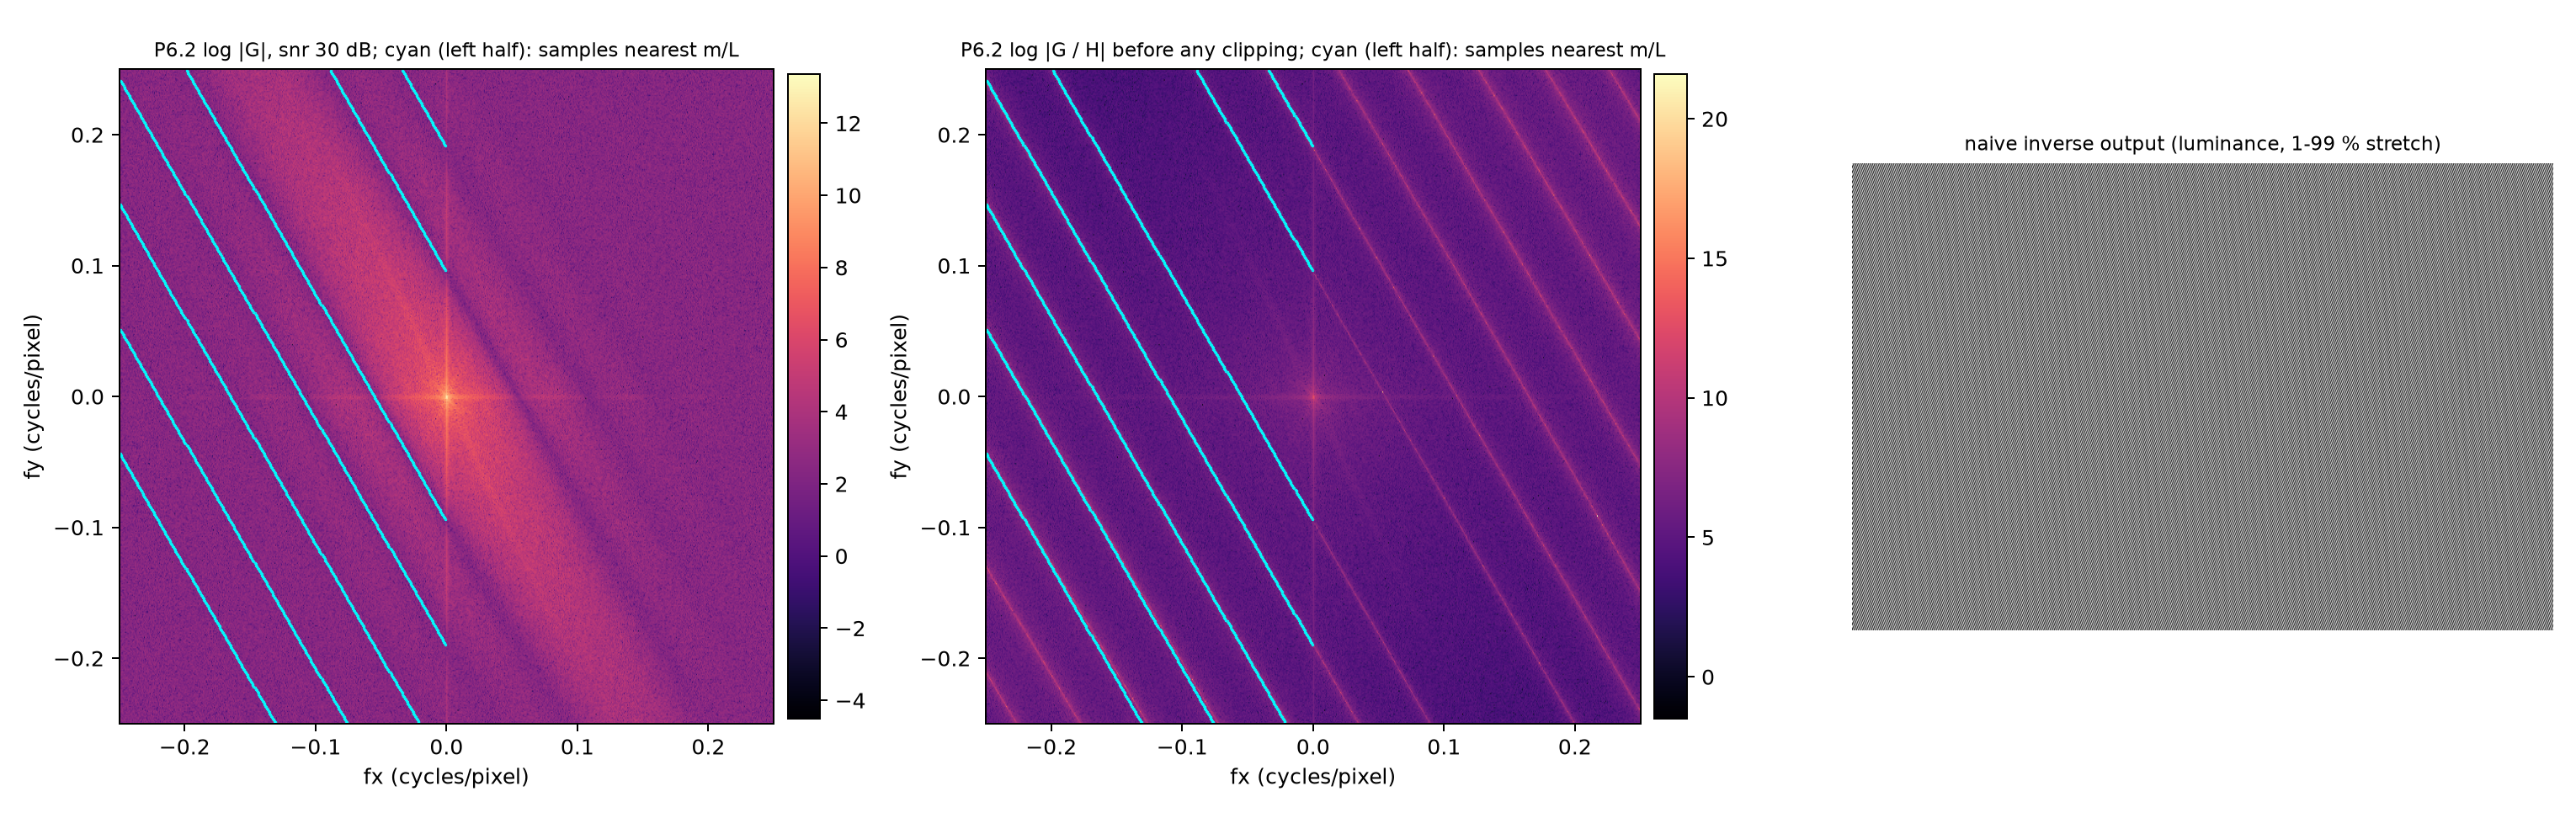
\includegraphics[width=\linewidth]{problem_6/inverse_spectrum.png}
\caption{At 30 dB: $\log|G|$, $\log|G/H|$ before any clipping, and the inverse
output, with $f_x,f_y$ in cycles/pixel. Cyan marks the sampled frequencies
nearest the predicted zeros in the left half; the right half shows the stripes
themselves.}
\label{fig:inverse}
\end{figure}

Since $G=HF+N$, the inverse gives $\hat F=F+N/H$: the image part comes back
exactly and the noise is divided by $H$. \textbf{Because $\hat F-F=N/H$, any
nonzero noise at a frequency where $|H|\to0$ is multiplied by $1/|H|\to\infty$,
so the error there can become arbitrarily large.}

In $\log|G|$ the zero lines are dark stripes perpendicular to the motion, partly
filled in by the noise floor. In $\log|G/H|$ the same lines become bright stripes
of amplified noise (Fig.~\ref{fig:inverse}). Near the zero lines the spectral
error is 28 times larger than away from them, at every SNR, because the error
$N/H$ is proportional to the noise and the ratio only depends on $|H|$. The
stripes repeat every $1/L$ along the motion direction, so the longer the blur,
the more zero lines cross the frequency plane and the more of the spectrum is
ruined. Even at 50 dB the output is pure amplified noise (4.47 dB, worse than
the blurred input).

\subsection{Wiener deconvolution}

\paragraph{Derivation.} Now $G=HF+N$ with $f$ and $n$ uncorrelated. The same
argument as in 5.1 with $\operatorname{E}[F\overline G]=\overline H S_{ff}$ and
$\operatorname{E}|G|^2=|H|^2S_{ff}+S_{nn}$ gives the linear MMSE filter
\begin{equation}
\hat F=\frac{\overline H\,S_{ff}}{|H|^2S_{ff}+S_{nn}}\,G=\frac{\overline H}{|H|^2+S_{nn}/S_{ff}}\,G
\;\approx\;\frac{\overline H(u,v)\,G(u,v)}{|H(u,v)|^2+K}.
\end{equation}
The last step replaces the frequency-dependent noise-to-signal ratio
$S_{nn}/S_{ff}$ by a single constant $K$. Images are in $[0,1]$ and the PSF sums
to one, so $H(0,0)=1$ and $K$ is a dimensionless noise-to-signal power ratio:
the DFT normalisation scales $S_{nn}$ and $S_{ff}$ by the same factor, which
cancels. Where $|H|^2\gg K$ the filter is the inverse $1/H$, and where
$|H|^2\ll K$ it tends to $\overline H/K\to0$ instead of blowing up.

\begin{table}[H]
\centering
\begin{tabular}{rrrrrrr}
\toprule
SNR (dB) & best $K$ & $10^{-\text{SNR}/10}$ & PSNR (dB) & SSIM & PSNR, $K=10^{-7}$ & PSNR, $K=1$\\
\midrule
50 & $1.58\times10^{-3}$ & $1.00\times10^{-5}$ & 31.261 & 0.8311 & 13.020 & 11.817\\
40 & $6.31\times10^{-3}$ & $1.00\times10^{-4}$ & 28.306 & 0.7003 & 7.046 & 11.817\\
30 & $2.51\times10^{-2}$ & $1.00\times10^{-3}$ & 25.825 & 0.5529 & 5.187 & 11.817\\
20 & $6.31\times10^{-2}$ & $1.00\times10^{-2}$ & 22.692 & 0.3460 & 4.679 & 11.814\\
\bottomrule
\end{tabular}
\caption{Wiener deconvolution with $K$ swept over 36 log-spaced values from
$10^{-7}$ to 1. PSNR and SSIM on outputs clipped to $[0,1]$, data range 1
(\code{k\_sweep.txt}).}
\label{tab:k}
\end{table}

\begin{figure}[H]
\centering
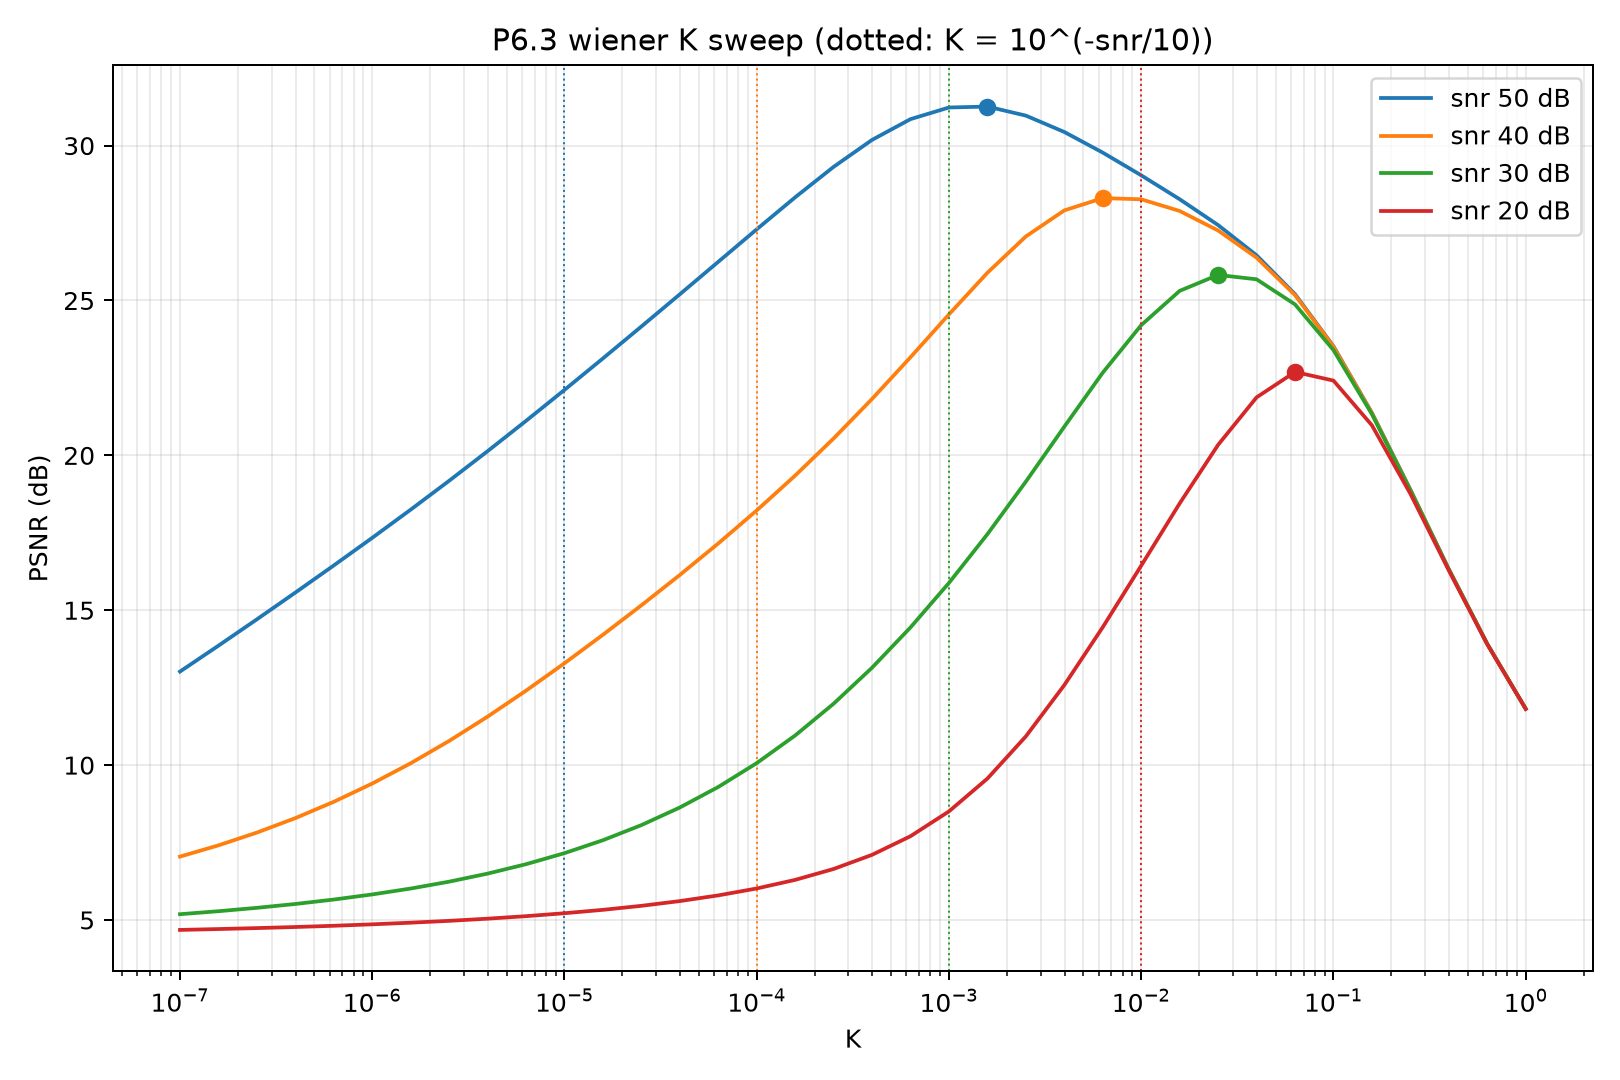
\includegraphics[width=0.68\linewidth]{problem_6/k_sweep.png}\\
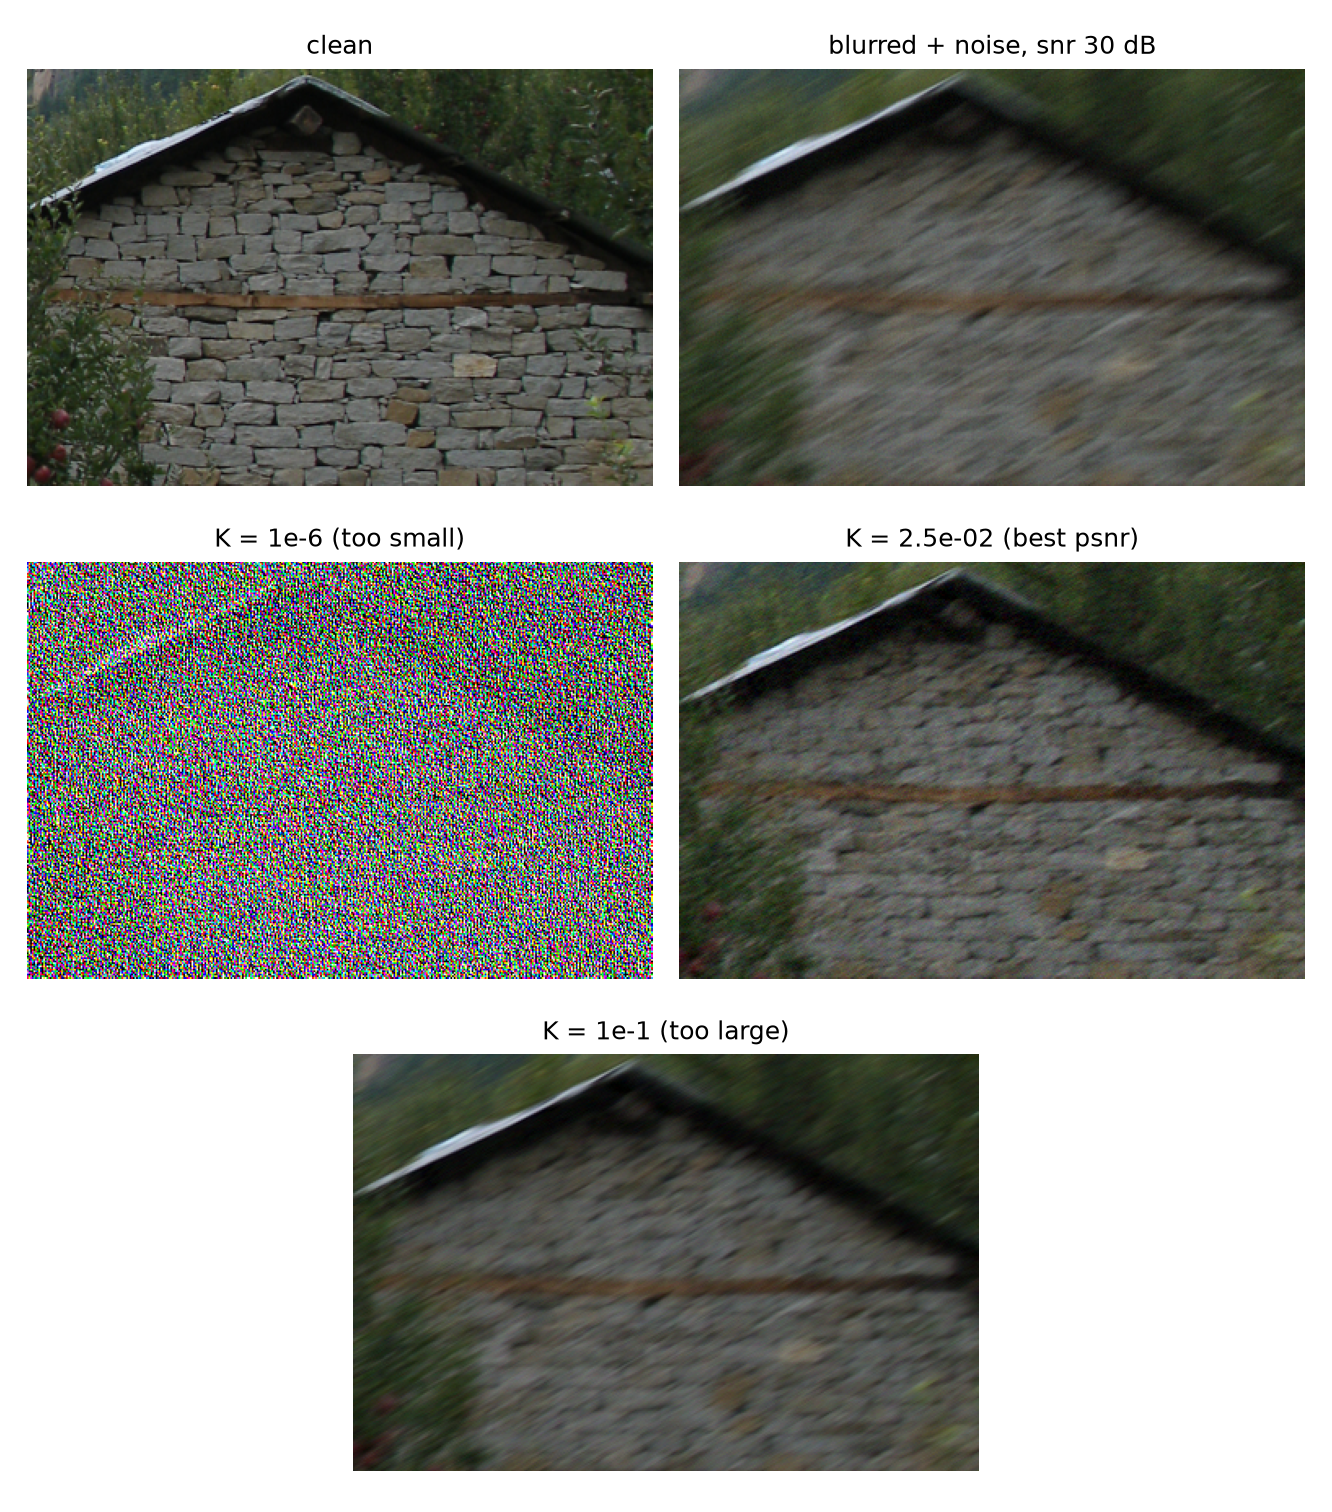
\includegraphics[width=\linewidth]{problem_6/deblurred_comparison.png}
\caption{Top: PSNR (dB) against $K$ for each SNR; dotted lines mark
$K=10^{-\text{SNR}/10}$. Bottom: roof crop at 30 dB with $K$ too small, best and
too large.}
\label{fig:k}
\end{figure}

A small $K$ brings back the inverse-filter failure: at $K=10^{-7}$ the PSNR is
4.7 to 13.0 dB and the output is dominated by amplified noise (Fig.~\ref{fig:k},
bottom). A large $K$ under-deconvolves: at $K=1$ the gain $\overline H/(|H|^2+1)$
is at most one half (exactly $1/2$ at DC), so the output is a dim, still blurred
image (11.8 dB). In between, each curve has a clear optimum, and it moves to
larger $K$ as the noise grows, from $1.6\times10^{-3}$ at 50 dB to
$6.3\times10^{-2}$ at 20 dB. The restored image gains 6.4 dB over the blurred
input at 50 dB but only 0.2 dB at 20 dB, where the noise leaves little to invert.

The best $K$ is much larger than the flat-spectrum guess $K=10^{-\text{SNR}/10}$
(the ratio of total noise power to total signal power): 158 times larger at
50 dB, falling to 6.3 times at 20 dB. $K$ stands in for $S_{nn}/S_{ff}(u,v)$ at
the frequencies where it matters, the ones where $|H|^2$ is about as large as
$K$. Those are middle and high frequencies, where a natural image has far less
power than its average (which is dominated by low frequencies), so the real
noise-to-signal ratio there is much higher than the global one. As the noise
grows, the deciding frequencies move down towards where the image power is
closer to its average, and the gap shrinks.

\subsection{Estimating and removing a real blur}

\paragraph{The photo.} I photographed the backlit keyboard of a laptop in a dim
room while moving the phone during the exposure (\code{photos/blur1.jpg},
$4032\times1816$ after the EXIF rotation). Of the four blurred shots I took, this
one has the straightest, most even streaks and the clearest blur signature. In two
of the others each key appears as several separate copies or the streaks are
kinked, and the estimator below returned a meaningless length of 4 pixels; in the
third the streaks are curved. A single straight PSF cannot describe any of those.
I also took a sharp photo of the same keyboard with the phone held still
(\code{photos/reference\_for\_blur.jpg}). It is not registered to the blurred
one, so I only use it as a control for the blur estimate, not to compute any
error. The photo is box-downsampled by 3 to $1344\times605$ so that the blur is a
few tens of pixels long and the FFTs are quick; all lengths below are at this
scale unless stated.

\paragraph{Why the stripes are perpendicular to the motion.} For a blurred photo
$|G|=|H|\,|F|$, and from 6.1 $|H|$ vanishes on the lines
$\mathbf f\cdot\mathbf u=m/L$, which are perpendicular to the motion direction
$\mathbf u$. Whatever the scene, the log spectrum therefore shows dark stripes
perpendicular to the motion, $1/L$ apart. The blur direction is the normal to the
stripes and the length is one over their spacing.

\paragraph{Estimating $\theta$ and $L$.} Taking the log of the spectrum separates
blur from scene, $\log|G|=\log|H|+\log|F|$, and $\log|H|$ repeats every $1/L$
along $\mathbf u$ (its value drops sharply at every zero line). The inverse
transform of $\log|G|$, the cepstrum, therefore has a strong negative spike at
distance $L$ from the origin in direction $\mathbf u$; this is the idea behind
Cannon's blur identification \cite{cannon}. \code{estimate\_blur} finds the most
negative cepstrum value at radius 3 to 80 in one half-plane (the cepstrum is
even) and refines its position with a three-point parabola along each axis.
Before that I multiply the image by a Hann window, so the jump at the image border
does not add a bright cross to the spectrum. On the synthetic blurred images (true
$\theta=30^\circ$, $L=21$) the estimator returns $\theta$ between $30.3^\circ$ and
$30.6^\circ$ and $L$ between 21.5 and 21.6 at all four SNRs
(\code{real\_blur.txt}). The length comes out about half a pixel long, which fits
the rasterised OTF departing from the ideal sinc at higher frequencies
(Fig.~\ref{fig:otf}).

On the photo it gives
\[
\theta=90.0^\circ,\qquad L=35.7\ \text{pixels}\ (107.2\text{ at full size}),\qquad 1/L=0.0280\ \text{cycles/pixel},
\]
with a cepstrum value of $-0.0363$ at the spike. The motion is vertical in the
frame, so the stripes should be horizontal, and they are: the red lines drawn at
$f_y=m/L$ in Fig.~\ref{fig:real-spectrum} sit on the dark bands of $\log|G|$. A
keyboard is a periodic pattern, so I checked that the spike is not caused by the
key spacing. In the sharp control photo the cepstrum at the same position is
$+0.0011$, i.e.\ there is nothing there. Its own most negative value is at a
different distance, 58.3 pixels along $90.1^\circ$, which I take to come from the
regular rows of keys.

\begin{figure}[H]
\centering
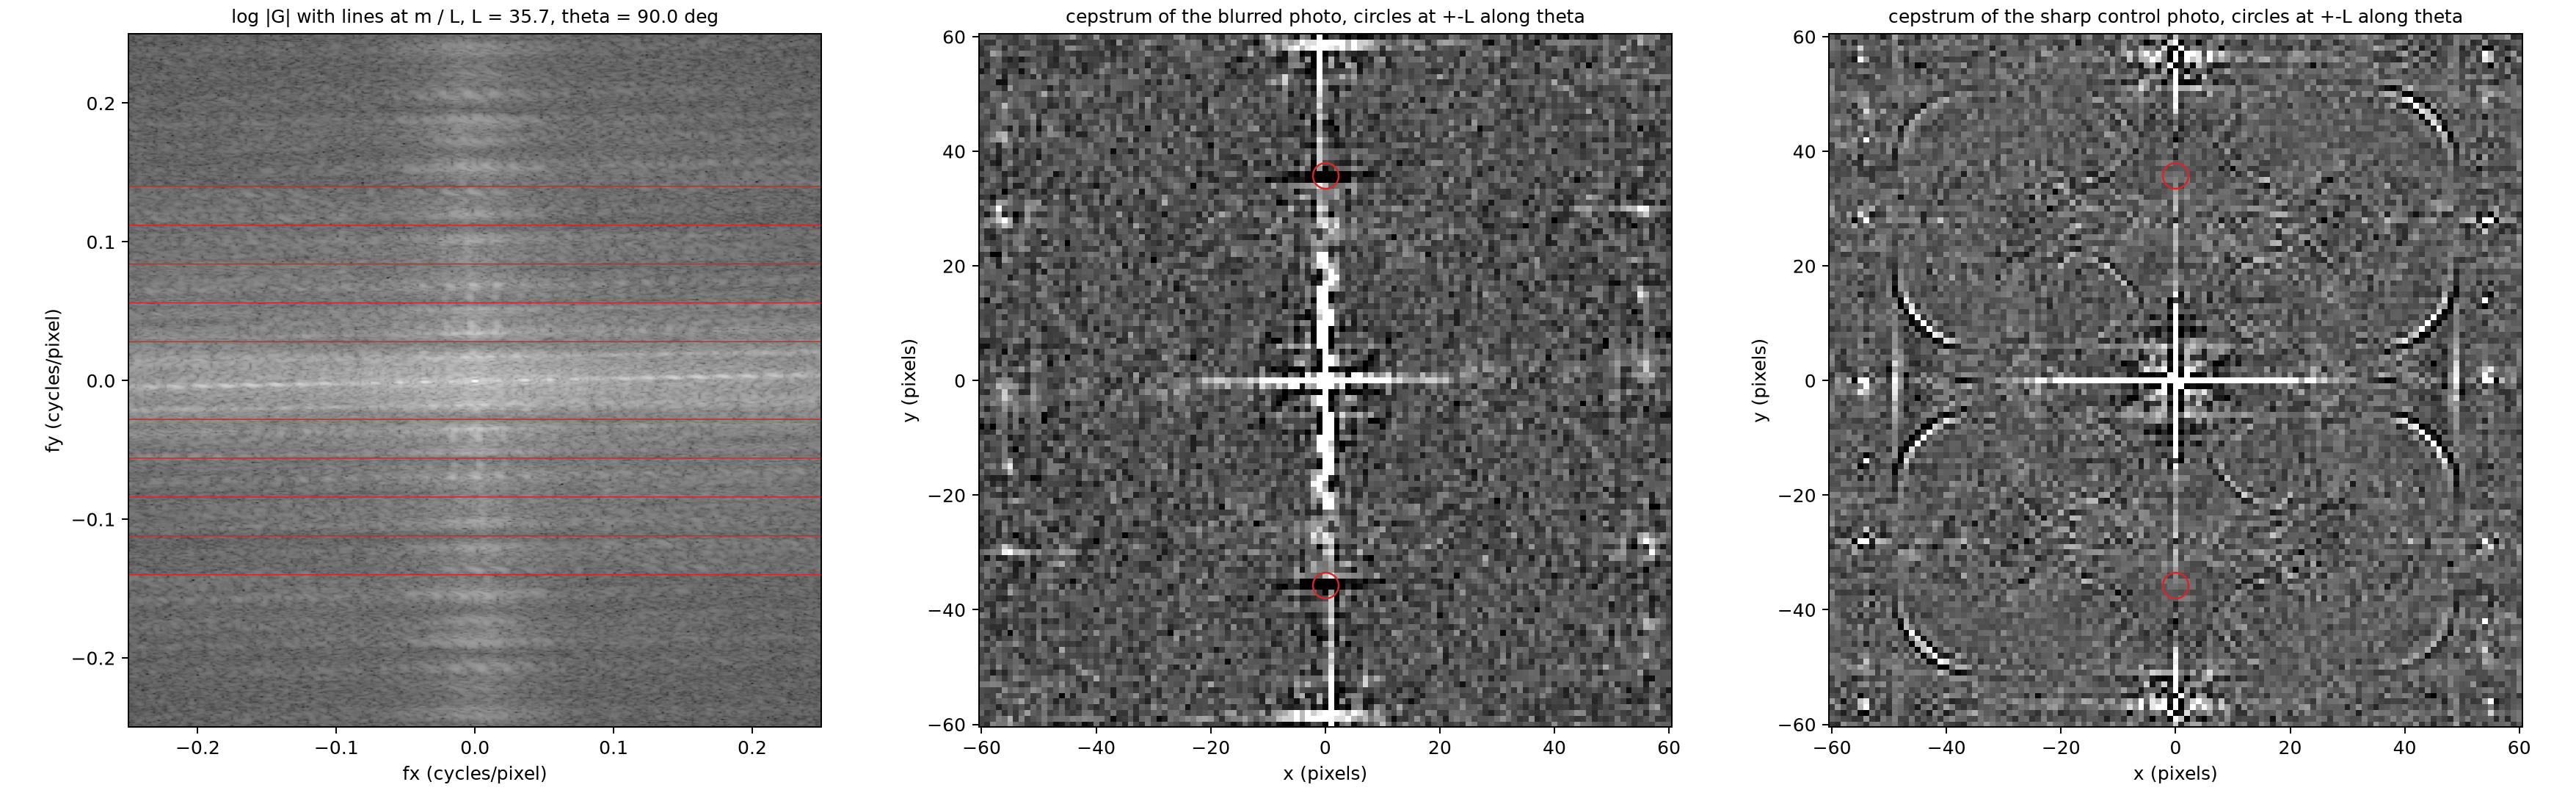
\includegraphics[width=\linewidth]{problem_6/real_blur_spectrum.png}
\caption{Left: $\log|G|$ of the Hann-windowed photo against $f_x,f_y$
(cycles/pixel), with red lines at the estimated stripe positions $f_y=\pm m/L$,
$m=1,\dots,5$. Middle: the cepstrum near the origin (pixels), with the spikes at
$\pm L$ circled. Right: the cepstrum of the sharp control photo, with nothing at
the same positions.}
\label{fig:real-spectrum}
\end{figure}

\paragraph{Deconvolution and the choice of $K$.} I built the PSF for
$\theta=90.0^\circ$, $L=35.7$ with \code{motion\_psf}, mirror-padded the photo by
$2L$ (a real blur is not circular, so circular wrap-around would add false
edges), and applied the Wiener filter for seven values of $K$. There is no clean
image to compute PSNR against, so I needed another way to pick $K$. I measured
how much the deconvolution raises the noise: the median ratio of the
plane-removed standard deviation after and before deconvolution, over the
flattest 10\,\% of the $32\times32$ tiles of the blurred photo
(Table~\ref{tab:real-k}). My rule was to take the smallest $K$ whose noise gain
is at most 2. I set this rule after a first look at a few restorations and a rough
noise check, so it states my choice precisely rather than testing it
independently. The rule gives $K=0.03$.

\begin{table}[H]
\centering
\begin{tabular}{rrrrr}
\toprule
$K$ & noise gain & outside $[0,1]$ & min & max\\
\midrule
$10^{-4}$ & 33.04 & 30.65\,\% & $-4.96$ & 10.10\\
$3\times10^{-4}$ & 20.19 & 23.23\,\% & $-4.03$ & 8.36\\
$10^{-3}$ & 11.00 & 18.10\,\% & $-2.95$ & 6.23\\
$3\times10^{-3}$ & 5.98 & 15.41\,\% & $-1.99$ & 4.45\\
$10^{-2}$ & 2.89 & 12.14\,\% & $-1.13$ & 3.05\\
$\mathbf{3\times10^{-2}}$ & \textbf{1.41} & \textbf{8.92\,\%} & $\mathbf{-0.65}$ & \textbf{2.12}\\
$10^{-1}$ & 0.62 & 5.95\,\% & $-0.29$ & 1.36\\
\bottomrule
\end{tabular}
\caption{Wiener $K$ sweep on the real photo (\code{real\_blur.txt}). Noise gain
is restored over blurred standard deviation in the flattest tiles; ``outside
$[0,1]$'' is the share of restored values below 0 or above 1. Bold: chosen.}
\label{tab:real-k}
\end{table}

\begin{figure}[H]
\centering
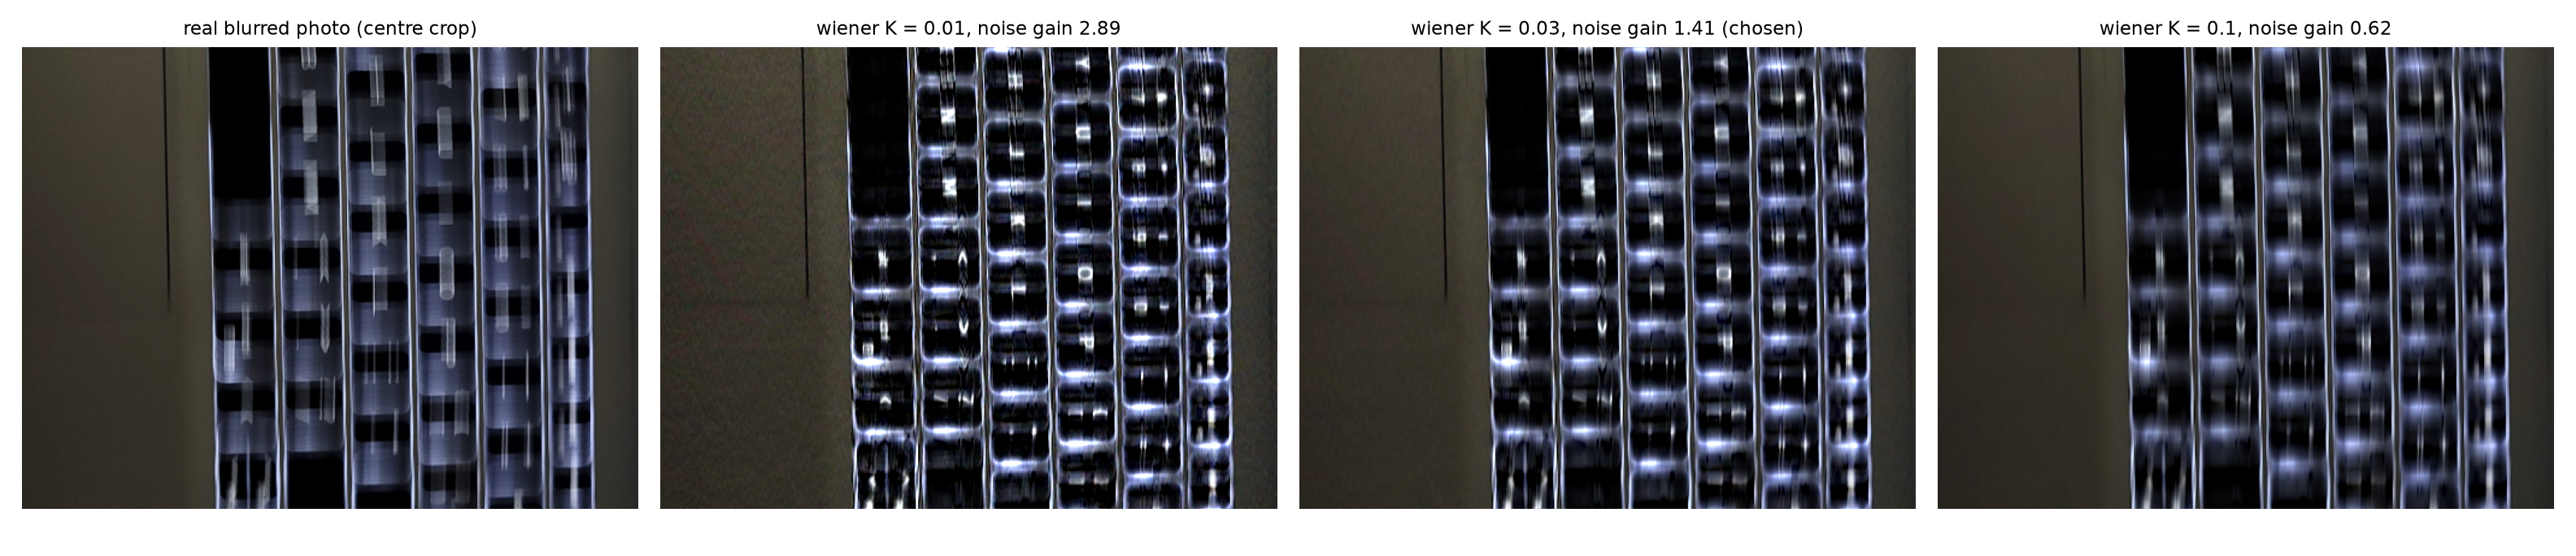
\includegraphics[width=\linewidth]{problem_6/real_blur_deblurred.png}
\caption{Centre crop of the blurred photo and the Wiener restorations with
$K=0.01$, 0.03 (chosen) and 0.1.}
\label{fig:real-deblur}
\end{figure}

In the centre of the photo the restoration works (Fig.~\ref{fig:real-deblur}).
The keys become separate rounded squares again, and several letters can be read.
$K=0.01$ recovers a little more letter detail, but its noise gain is 2.89 and
the ringing around the keys is stronger; $K=0.1$ keeps the noise below the
blurred photo's but leaves the letters smeared. The table also shows how hard the
filter pushes: even at $K=0.03$, 8.9\,\% of the restored values fall outside
$[0,1]$. Of those, 94.3\,\% are below zero, and 72.7\,\% of the negative ones
are where the blurred photo is darker than 0.1, i.e.\ ringing pushes the dark
key areas under black.

\paragraph{Artifacts and what causes them.} The restoration is not equally good
everywhere, and two things stand out: dark and bright bands below the bright
lower edge of the keyboard (Fig.~\ref{fig:real-echo}), and streaks that stay in the
top third of the frame (Fig.~\ref{fig:real-regions}). I ran two checks to find out
which of them comes from the model being wrong and which comes from the method.

\emph{The bands below the keyboard edge.} On the dark area below the brightest
edge in the photo, the restored image has a dark band 24 rows below the edge and
a bright one 40 rows below it, where the blurred photo is smooth. The pattern
repeats on a scale of about one blur length. To see whether a wrong PSF causes them, I made
a control in which the model holds exactly: my sharp photo of the same keyboard,
blurred with the estimated PSF, plus white noise at the photo's own level
($\sigma=1.21$ grey levels, measured in its flattest tiles), restored with the same
$K$. The control gets the same bands in nearly the same places (dark at 18 and
bright at 38 rows below its edge, against 24 and 40 for the photo), so they are not
a sign that the PSF is wrong. They come from inverting a blur whose transfer function
has zero lines. The model says the frequencies on the lines $f_y=m/L$ were
multiplied by zero, so the photo holds no information there, and a linear filter
can only leave those frequencies out or amplify the noise that sits there. A sharp
edge that is missing a comb of frequencies spaced $1/L$ apart comes back with
copies of itself spaced about $L$ apart. The bands are strongest at this edge
because it is the highest-contrast edge in the photo. Raising $K$ weakens them,
because the gain next to a zero line can never exceed $1/(2\sqrt K)$, but it also
sharpens less:

\begin{center}
\begin{tabular}{lrrrrr}
\toprule
& edge step & blurred & $K=0.01$ & $K=0.03$ & $K=0.1$\\
\midrule
real photo & 0.191 & 0.0057 & 0.0348 & 0.0302 & 0.0204\\
control (exact blur) & 0.038 & 0.0047 & 0.0157 & 0.0128 & 0.0094\\
\bottomrule
\end{tabular}
\end{center}

The numbers are the RMS of the row profile 14 to 94 rows below the edge (central
half of the columns, straight line removed), in luminance on $[0,1]$
(\code{real\_blur.txt}). The control's edge step is five times smaller than the
photo's, so its bands are weaker too.

\emph{The blur changes across the frame.} Running the estimator on parts of the
photo gives:

\begin{center}
\begin{tabular}{lrr}
\toprule
region & $\theta$ (deg) & $L$ (px)\\
\midrule
top third & 96.4 & 36.6\\
middle third & 90.2 & 35.6\\
bottom third & 84.9 & 36.6\\
left half & 89.2 & 35.5\\
right half & 90.4 & 36.0\\
\bottomrule
\end{tabular}
\end{center}

The length is about the same everywhere, but the direction turns by $11.5^\circ$
from the top third to the bottom third, while the left and right halves agree.
This is the real model failure in this photo: the linear, spatially invariant model
assumes one PSF for the whole image, and here the blur is different at the top and
the bottom. A small rotation of the phone about the viewing axis (a roll) during
the exposure, on top of the vertical movement, would produce exactly this pattern.
A roll by an angle $\phi$ about the frame centre moves a point at height $y$
sideways by $\phi y$, which tilts a vertical streak of length $L$ by about
$\phi y/L$. The centres of the top and bottom thirds are 448 pixels from the
middle and their streaks tilt by about $5.75^\circ$, so
$\phi\cdot448\approx35.7\tan5.75^\circ=3.6$ pixels, i.e.\ $\phi\approx0.46^\circ$.
This roll is my interpretation: it fits the measured pattern, but I did not
measure how the phone moved.

The middle third, where the local estimate agrees with the global PSF, is restored
best, while the top third keeps streaks (Fig.~\ref{fig:real-regions}, middle row).
Restoring each third with its own estimated PSF did not visibly fix the top third
(bottom row) and did not reduce the bands at the bottom edge either (0.0311 with
the bottom third's own PSF against 0.0302 with the global one). So a straight
streak at constant speed is not a good description of the local blur at the top
either. With a rolling phone the direction and speed of each point can change
during the exposure, but from this photo alone I cannot tell which of these fails.

Clipped highlights are another limit of the linear model, since a saturated pixel
no longer equals the sum of light the model assumes. Here, though, only 0.14\,\% of
the full-size pixels have a channel at 254 or 255, and only 1.8\,\% of the restored
pixels with a value outside $[0,1]$ lie within one blur length (along the motion)
of a clipped pixel, so clipping is not the main problem in this photo. Since there
is no sharp, registered original, the judgement of the restored image is visual,
and I report no PSNR or SSIM.

\begin{figure}[H]
\centering
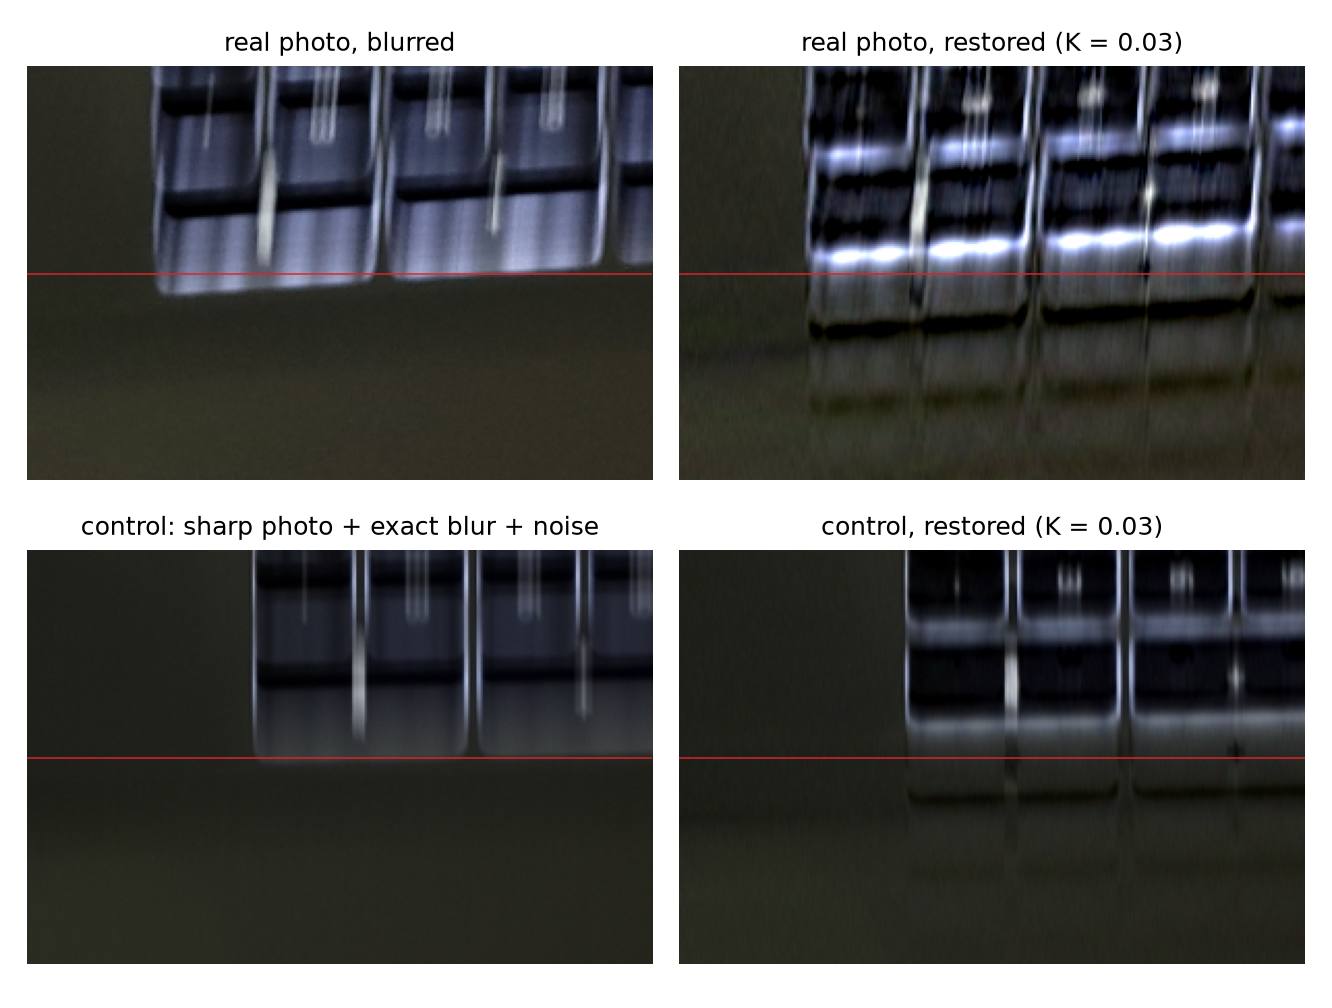
\includegraphics[width=\linewidth]{problem_6/real_blur_echo.png}
\caption{Bands below the brightest edge. From left: the blurred photo and its
restoration ($K=0.03$), and the control (my sharp photo of the keyboard blurred
with the estimated PSF plus white noise at the photo's level) and its restoration.
The red line marks the edge; both restorations show a dark band about 20 rows and a
bright band about 40 rows below it (24 and 40 rows in the photo, 18 and 38 in the
control).}
\label{fig:real-echo}
\end{figure}

\begin{figure}[H]
\centering
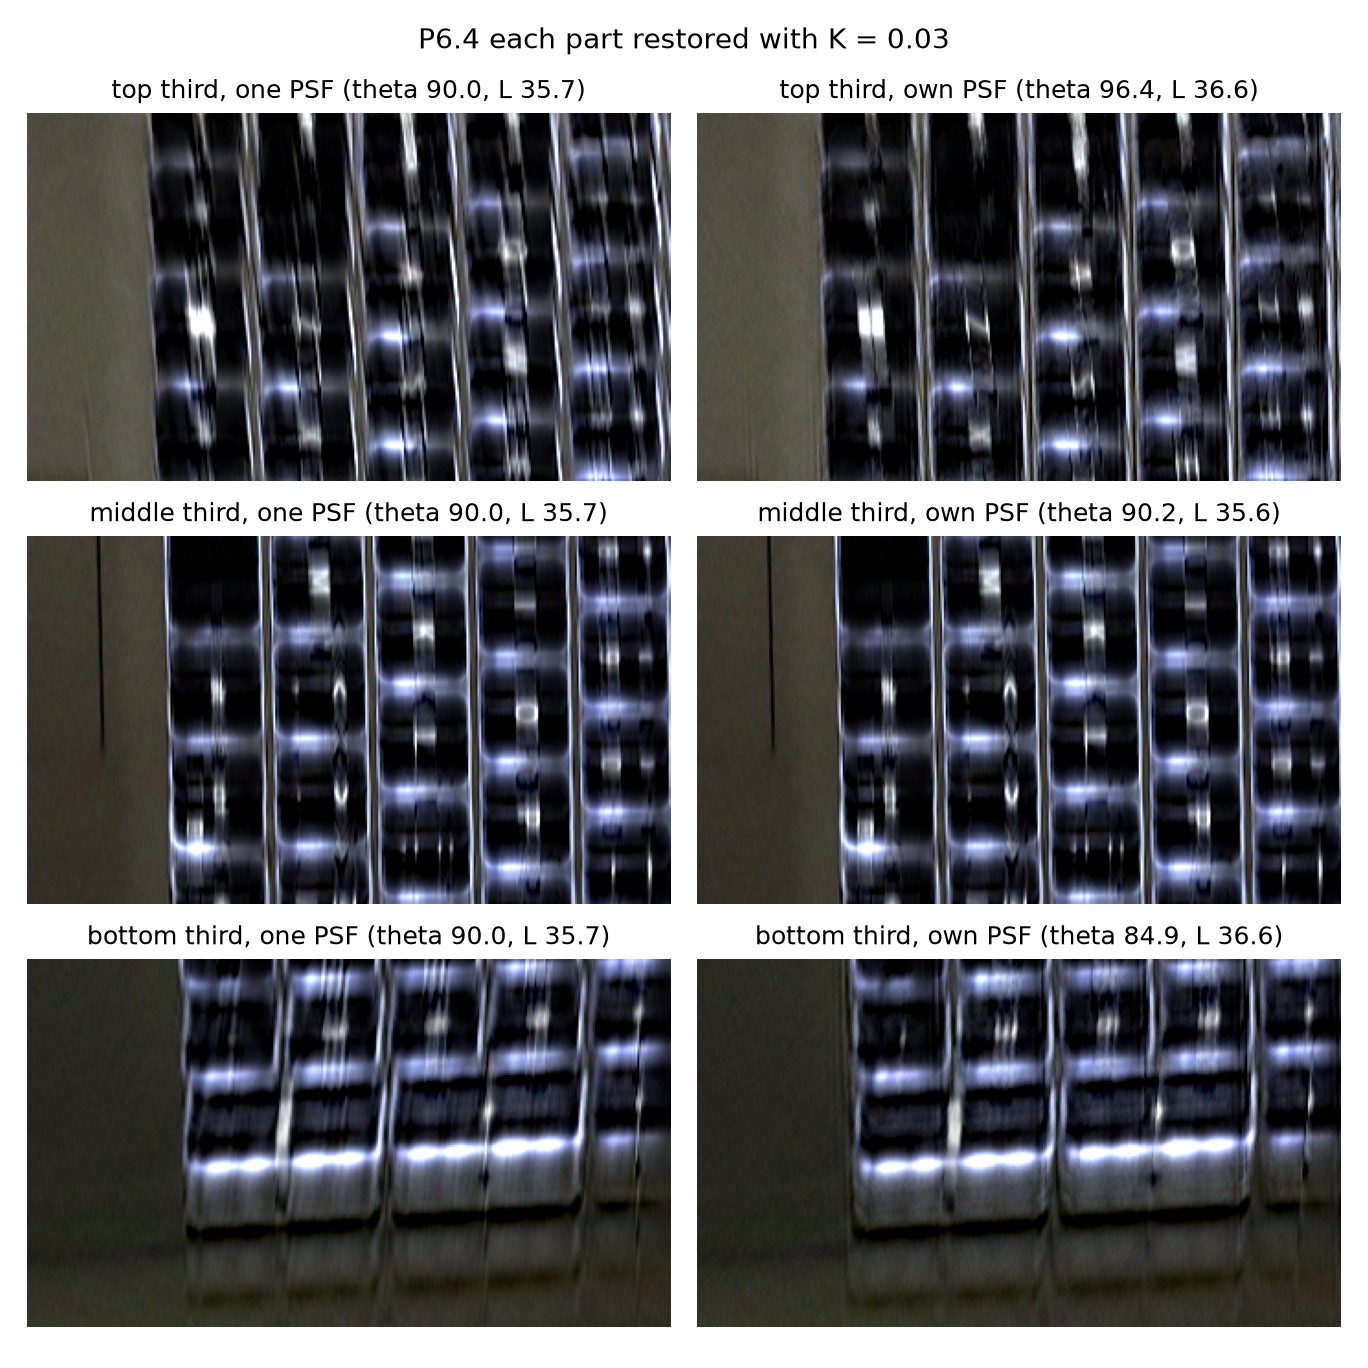
\includegraphics[width=\linewidth]{problem_6/real_blur_regions.png}
\caption{Top row: crops from the top, middle and bottom thirds of the blurred
photo, with the blur direction and length estimated on each third. Middle row: the
same crops restored with the single global PSF ($\theta=90.0^\circ$, $L=35.7$,
$K=0.03$). Bottom row: each third restored with its own estimated PSF. The middle
third is restored best; the top third keeps streaks with either PSF.}
\label{fig:real-regions}
\end{figure}

\begin{thebibliography}{9}

\bibitem{gonzalez}
R.~C. Gonzalez and R.~E. Woods, \emph{Digital Image Processing}, 4th ed.
Pearson, 2018.

\bibitem{oppenheim}
A.~V. Oppenheim and J.~S. Lim, ``The importance of phase in signals,''
\emph{Proceedings of the IEEE}, vol.~69, no.~5, pages 529 to 541, 1981.

\bibitem{tomasi}
C.~Tomasi and R.~Manduchi, ``Bilateral filtering for gray and color images,'' in
\emph{Proc. IEEE International Conference on Computer Vision}, 1998,
pages 839 to 846, doi:10.1109/ICCV.1998.710815.

\bibitem{kuwahara}
M.~Kuwahara, K.~Hachimura, S.~Eiho and M.~Kinoshita, ``Processing of
RI-angiocardiographic images,'' in K.~Preston and M.~Onoe (eds.), \emph{Digital
Processing of Biomedical Images}, 1976, pages 187 to 202,
doi:10.1007/978-1-4684-0769-3\_13.

\bibitem{immerkaer}
J.~Immerkær, ``Fast noise variance estimation,'' \emph{Computer Vision and Image
Understanding}, vol.~64, no.~2, pages 300 to 302, 1996, doi:10.1006/cviu.1996.0060.

\bibitem{wang}
Z.~Wang, A.~C. Bovik, H.~R. Sheikh and E.~P. Simoncelli, ``Image quality
assessment: from error visibility to structural similarity,'' \emph{IEEE
Transactions on Image Processing}, vol.~13, no.~4, pages 600 to 612, 2004,
doi:10.1109/TIP.2003.819861.

\bibitem{cannon}
M.~Cannon, ``Blind deconvolution of spatially invariant image blurs with phase,''
\emph{IEEE Transactions on Acoustics, Speech, and Signal Processing}, vol.~24,
no.~1, pages 58 to 63, 1976, doi:10.1109/TASSP.1976.1162770.

\end{thebibliography}

\appendix
\section{Dated predictions}

These are my two prediction files as committed on 23 October 2026, before the
experiments they predict: \code{3c9e956} at 16:29:03 IST for both files, and
\code{4acb1a0} at 16:29:11 IST, which only corrected the time in the first line
of the 2.2 file from 16:31 to 16:29. Neither file was changed after that, and the
originals are in the git history. They were written in Markdown with plain-text
maths; below they are converted to \LaTeX\ without changing any words. The same
text is in \code{docs/predictions/} as PDF files.

\small
\subsection{1.2 prediction: test-image phase with white-noise magnitude}\label{app:pred-phase}

written 2026-10-23 16:28 IST, before any phase/magnitude code was written or run. this file is not edited after the experiment. discrepancies go in the report.

\subsubsection*{setup}

f is the 512 x 512 test image \texttt{q1.png}, N = 512, F = \textbar{}F\textbar{} e\textasciicircum{}\{j phi\}. n is uniform white noise, n(x, y) \textasciitilde{} U[0, 1] i.i.d., with dft N\_n(u, v). the reconstruction is

\begin{verbatim}
r = idft{ |N_n(u, v)| e^{j phi(u, v)} }.
\end{verbatim}

\subsubsection*{derivation}

\textbf{1. statistics of the noise magnitude.} for (u, v) != (0, 0), N\_n(u, v) is a sum of N\textasciicircum{}2 i.i.d. terms times unit phasors, so by the central limit theorem it is close to a circular complex gaussian with E\textbar{}N\_n\textbar{}\textasciicircum{}2 = N\textasciicircum{}2 var(n) = N\textasciicircum{}2 / 12. its magnitude is then rayleigh distributed. writing \textbar{}N\_n\textbar{} = mu (1 + eps),

\begin{verbatim}
E[eps] = 0,  var[eps] = var|N_n| / mu^2 = (1 - pi/4) / (pi/4) = 4/pi - 1 = 0.273.
\end{verbatim}

since n is real, \textbar{}N\_n(u, v)\textbar{} = \textbar{}N\_n(-u, -v)\textbar{}, so eps is even-symmetric, and eps at different frequencies is (nearly) uncorrelated. the dc term N\_n(0, 0) = sum n \textasciitilde{} N\textasciicircum{}2 / 2 is deterministic in practice, and phi(0, 0) = 0 because f \textgreater{} 0, so the dc term only adds a constant offset to r.

\textbf{2. superposition.} by linearity of the inverse dft,

\begin{verbatim}
r = mu * p + mu * q + const,
p = idft{ e^{j phi} },          (flat-magnitude, phase-only image, task 1.2a)
q = idft{ eps e^{j phi} } = p (*) e,   e = idft{ eps },
\end{verbatim}

where (*) is circular convolution (convolution theorem: a product of spectra is a circular convolution in space).

\textbf{3. what p looks like (shift theorem).} think of f as a superposition of localised features (edge segments, corners, thin lines) at positions (x\_k, y\_k). by the shift theorem each feature's spectrum carries the linear phase factor exp(-j 2 pi (u x\_k + v y\_k) / N). phase-only reconstruction keeps these factors and throws away the magnitude. a pure linear phase with flat magnitude inverts to an impulse at the same place:

\begin{verbatim}
idft{ exp(-j 2 pi (u x_k + v y_k) / N) } = delta(x - x_k, y - y_k).
\end{verbatim}

so the energy of p collects at the positions of the features of f, not at random positions. equivalently p = f (*) idft\{1 / \textbar{}F\textbar{}\}. natural-image spectra fall roughly like 1 / rho\textasciicircum{}alpha with alpha around 1 to 2, so dividing by \textbar{}F\textbar{} is a whitening high-pass that boosts high frequencies roughly like rho\textasciicircum{}alpha. smooth shading is suppressed and the places where many frequencies are in phase (edges, lines, corners) survive.

prediction for p (1.2a): the outlines of the photographer, the coat edge, the tripod legs, the camera and the buildings on the horizon appear as thin signed lines (bright on one side, dark on the other), at their correct positions. flat areas (sky, the coat interior, the grass at coarse scale) go to a uniform mid grey. the overall brightness pattern of the photo (dark coat, bright sky) is lost. the grass texture survives as fine high-frequency texture, because it is full of small edges.

\textbf{4. what q adds (noise magnitude case).} e = idft\{eps\} is a real, even, white-like random field with no spatial structure. convolving p with it spreads each feature's energy over the whole image with random weights, so q is a stationary speckle-like texture that is not concentrated at the edges. by parseval, the energy ratio of the two terms (dc excluded) is

\begin{verbatim}
energy(q) / energy(p) = mean(eps^2) = 4/pi - 1 = 0.273,
\end{verbatim}

i.e. a structured-to-speckle energy ratio of about 3.7 (5.6 dB).

prediction for r: the same edge map as p, recognisable, but with visible grainy speckle over the whole frame, flat regions included. if r (dc removed) is fitted by least squares as r = c p + residual, then

\begin{verbatim}
energy(residual) / energy(c p) ~ 0.27,
corr(r, p) ~ 1 / sqrt(1 + 0.273) ~ 0.89.
\end{verbatim}

the image will not look like a noisy copy of the photograph, it will look like a noisy edge drawing of it.

\subsubsection*{1.2b prediction: original magnitude, zero phase}

setting phi = 0 gives r\_0 = idft\{ \textbar{}F\textbar{} \}. \textbar{}F\textbar{} is real and even (\textbar{}F(u, v)\textbar{} = \textbar{}F(-u, -v)\textbar{} for real f), so r\_0 is real and even: r\_0(x, y) = r\_0(-x, -y) (mod N), i.e. point-symmetric about the origin. all cosines peak together at the origin, so r\_0 is a sharp peak at (0, 0) (the corners of the unshifted array, the centre after fftshift) with height sum \textbar{}F\textbar{} / N\textasciicircum{}2, falling off quickly. the periodic extension of the photo has strong discontinuities at the image border, which puts extra energy along the u = 0 and v = 0 axes, so the peak should have a faint horizontal and vertical cross through it. nothing of the photographer's shape will be recognisable, because the positions of features live in the phase, which is now gone.

\subsection{2.2 prediction: ringing of the step-edge image}\label{app:pred-ringing}

written 2026-10-23 16:29 IST, before any filtering code for problem 2 was written or run. this file is not edited after the experiment.

\subsubsection*{setup}

s(x, y) is 512 x 512, a square of side 256 and intensity B = 200 centred on a background A = 50. the square covers rows and columns 128 to 383, so its left edge lies between columns 127 and 128, at x\_e = 127.5. it is zero-padded to P = 1024 and filtered with a centred, real, zero-phase H. the profile is a row through the middle of the square (row 255), far from the corners. u is the frequency index measured from the centre of the padded spectrum, so index u means u / P cycles per pixel.

\subsubsection*{the 1-d reduction}

near the middle row and away from the corners the image looks like a function of x only. an image that varies only in x has a fourier transform confined to the line v = 0: if f(x, y) = g(x), then F(u, v) = G(u) * P * delta(v). the filter then acts only through its slice H(u, 0), and the filtered row is the 1-d convolution of g with h\_1(x) = ift\{ H(u, 0) \}.

\subsubsection*{ideal low-pass}

the slice of the ideal filter is H(u, 0) = 1 for \textbar{}u\textbar{} \textless{}= D0, else 0, i.e. a cutoff of f\_c = D0 / P cycles per pixel. in the continuous model

\begin{verbatim}
h_1(x) = 2 f_c sinc(2 f_c x) = sin(2 pi f_c x) / (pi x).
\end{verbatim}

a step of height (B - A) at x\_e has response

\begin{verbatim}
g(x) = A + (B - A) [ 1/2 + (1/pi) Si(2 pi f_c (x - x_e)) ],
Si(z) = integral_0^z sin(t) / t dt.
\end{verbatim}

Si has its global maximum at z = pi, where Si(pi) = 1.851937. so

\textbf{(i) overshoot}

\begin{verbatim}
OS = 100 (max g - B) / (B - A) = 100 (Si(pi)/pi - 1/2) = 8.95 %,
\end{verbatim}

independent of D0 and P (gibbs). with B - A = 150 the peak is at about 200 + 13.4 = 213.4.

\textbf{(ii) distance from the edge to the first overshoot peak}

\begin{verbatim}
2 pi f_c d = pi  ->  d = 1 / (2 f_c) = P / (2 D0) pixels.
\end{verbatim}

\begin{tabular}{lrrrr}
\hline
D0 & 10 & 20 & 40 & 80 \\
\hline
predicted OS (\%) & 8.95 & 8.95 & 8.95 & 8.95 \\
predicted d = P / (2 D0) (px) & 51.2 & 25.6 & 12.8 & 6.4 \\
\hline
\end{tabular}

\subsubsection*{expected sources of discrepancy (also predicted before running)}

\begin{enumerate}
\item \textbf{discrete passband.} on the P grid the ideal slice keeps the 2 D0 + 1 integer frequencies \textbar{}u\textbar{} \textless{}= D0. the kernel is then a dirichlet kernel, h[x] = sin(pi (2 D0 + 1) x / P) / (P sin(pi x / P)), whose first zero is at x = P / (2 D0 + 1). the overshoot peak sits at that zero, so the discrete prediction is d = P / (2 D0 + 1) = 48.8, 25.0, 12.6, 6.4 px. the overshoot of a dirichlet partial sum tends to the same 8.95 \% as the number of terms grows.
\item \textbf{sampling of the profile.} the edge is at x\_e = 127.5 and the profile is only known at integer columns, so a measured d is a half-integer and can be off by up to 0.5 px. the sampled maximum can also miss the true peak, which lowers the measured OS slightly, most for D0 = 80 where the peak is narrow.
\item \textbf{other edges.} the square is finite, and the zero padding adds a jump of -50 at the image border, 128 px from each square edge. for large z, Si(z) \textasciitilde{} pi/2 - cos(z)/z, so the ripple from an edge at distance r has amplitude about P / (2 pi\textasciicircum{}2 D0 r) of that edge's jump. for D0 = 10 this is about 2 \% of the jump for the opposite edge (r = 256) and 1.4 \% for the border jump (r = 128, jump 50). these ripples add or subtract depending on phase, so at D0 = 10 the measured OS can differ from 8.95 \% by a few percentage points, and the difference should shrink roughly like 1 / D0.
\item \textbf{the image is not really 1-d.} the square is only 256 px tall, so its spectrum is spread over a band of v around 0, of width about P / 256 = 4 bins. on the slice at height v the ideal cutoff is sqrt(D0\textasciicircum{}2 - v\textasciicircum{}2) \textless{} D0, which matters most at D0 = 10. the top and bottom edges also send their own ripple down to the middle row. both effects again fade as D0 grows.
\item \textbf{near a corner} the 1-d reduction fails completely: the local image varies in both x and y, its spectrum is not on the v = 0 line, and the 2-d ideal kernel is a jinc whose rings are circular. ripples from the vertical and horizontal edges overlap there, so the profile near a corner should show a different overshoot and a different peak position.
\end{enumerate}

\subsubsection*{gaussian low-pass}

H(u, 0) = exp(-u\textasciicircum{}2 / (2 D0\textasciicircum{}2)). its inverse transform is again a gaussian,

\begin{verbatim}
h_1(x) = exp(-x^2 / (2 sigma_s^2)) / (sqrt(2 pi) sigma_s),
sigma_s = P / (2 pi D0),
\end{verbatim}

which is positive everywhere and integrates to one. the edge response is

\begin{verbatim}
g(x) = A + (B - A) Phi((x - x_e) / sigma_s),
\end{verbatim}

with Phi the standard normal cdf. this is monotone, so

\textbf{predicted gaussian overshoot: OS = 0 \% for every D0.}

the transition just gets wider as D0 drops (10 \% to 90 \% width 2.56 sigma\_s = 2.56 P / (2 pi D0)). on the discrete grid the slice is cut off at \textbar{}u\textbar{} = P/2 = 512, where it is exp(-512\textasciicircum{}2 / (2 D0\textasciicircum{}2)), which is far below float64 precision for D0 \textless{}= 160, so the discrete kernel stays non-negative to round-off and OS should be 0 up to about 1e-10 \%.

\subsubsection*{butterworth (not required, written for 2.2b)}

for n = 1 the slice 1 / (1 + (u/D0)\textasciicircum{}2) is a lorentzian whose inverse transform is a two-sided exponential, positive everywhere, so OS = 0. for n \textgreater{}= 2 the kernel has negative lobes and OS \textgreater{} 0, growing with n toward the ideal-filter limit of 8.95 \% as n -\textgreater{} infinity, since the butterworth slice tends to the ideal box.

\normalsize

\end{document}
